%  LaTeX support: latex@mdpi.com 
%  For support, please attach all files needed for compiling as well as the log file, and specify your operating system, LaTeX version, and LaTeX editor.

%=================================================================
% DRAFT MODE: Uncomment next line for fast compilation (images as boxes)
%\documentclass[journal,article,submit,pdftex,moreauthors,draft]{Definitions/mdpi} 
\documentclass[journal,article,submit,pdftex,moreauthors]{Definitions/mdpi} 
%\documentclass[preprints,article,submit,pdftex,moreauthors]{Definitions/mdpi} 
% For posting an early version of this manuscript as a preprint, you may use "preprints" as the journal. Changing "submit" to "accept" before posting will remove line numbers.

%--------------------
% Class Options:
%--------------------
%----------
% journal
%----------
% Choose between the following MDPI journals:
% accountaudit, acoustics, actuators, addictions, adhesives, admsci, adolescents, aerobiology, aerospace, agriculture, agriengineering, agrochemicals, agronomy, ai, air, algorithms, allergies, alloys, amh, analytica, analytics, anatomia, anesthres, animals, antibiotics, antibodies, antioxidants, applbiosci, appliedchem, appliedmath, appliedphys, applmech, applmicrobiol, applnano, applsci, aquacj, architecture, arm, arthropoda, arts, asc, asi, astronomy, atmosphere, atoms, audiolres, automation, axioms, bacteria, batteries, bdcc, behavsci, beverages, biochem, bioengineering, biologics, biology, biomass, biomechanics, biomed, biomedicines, biomedinformatics, biomimetics, biomolecules, biophysica, biosensors, biosphere, biotech, birds, blockchains, bloods, blsf, brainsci, breath, buildings, businesses, cancers, carbon, cardiogenetics, catalysts, cells, ceramics, challenges, chemengineering, chemistry, chemosensors, chemproc, children, chips, cimb, civileng, cleantechnol, climate, clinbioenerg, clinpract, clockssleep, cmd, cmtr, coasts, coatings, colloids, colorants, commodities, complications, compounds, computation, computers, condensedmatter, conservation, constrmater, cosmetics, covid, crops, cryo, cryptography, crystals, csmf, ctn, curroncol, cyber, dairy, data, ddc, dentistry, dermato, dermatopathology, designs, devices, diabetology, diagnostics, dietetics, digital, disabilities, diseases, diversity, dna, drones, dynamics, earth, ebj, ecm, ecologies, econometrics, economies, education, eesp, ejihpe, electricity, electrochem, electronicmat, electronics, encyclopedia, endocrines, energies, eng, engproc, ent, entomology, entropy, environments, epidemiologia, epigenomes, esa, est, famsci, fermentation, fibers, fintech, fire, fishes, fluids, foods, forecasting, forensicsci, forests, fossstud, foundations, fractalfract, fuels, future, futureinternet, futureparasites, futurepharmacol, futurephys, futuretransp, galaxies, games, gases, gastroent, gastrointestdisord, gastronomy, gels, genealogy, genes, geographies, geohazards, geomatics, geometry, geosciences, geotechnics, geriatrics, glacies, grasses, greenhealth, gucdd, hardware, hazardousmatters, healthcare, hearts, hemato, hematolrep, heritage, higheredu, highthroughput, histories, horticulturae, hospitals, humanities, humans, hydrobiology, hydrogen, hydrology, hygiene, idr, iic, ijerph, ijfs, ijgi, ijmd, ijms, ijns, ijpb, ijt, ijtm, ijtpp, ime, immuno, informatics, information, infrastructures, inorganics, insects, instruments, inventions, iot, j, jal, jcdd, jcm, jcp, jcs, jcto, jdad, jdb, jeta, jfb, jfmk, jimaging, jintelligence, jlpea, jmahp, jmmp, jmms, jmp, jmse, jne, jnt, jof, joitmc, joma, jop, jor, journalmedia, jox, jpbi, jpm, jrfm, jsan, jtaer, jvd, jzbg, kidney, kidneydial, kinasesphosphatases, knowledge, labmed, laboratories, land, languages, laws, life, lights, limnolrev, lipidology, liquids, literature, livers, logics, logistics, lubricants, lymphatics, machines, macromol, magnetism, magnetochemistry, make, marinedrugs, materials, materproc, mathematics, mca, measurements, medicina, medicines, medsci, membranes, merits, metabolites, metals, meteorology, methane, metrics, metrology, micro, microarrays, microbiolres, microelectronics, micromachines, microorganisms, microplastics, microwave, minerals, mining, mmphys, modelling, molbank, molecules, mps, msf, mti, multimedia, muscles, nanoenergyadv, nanomanufacturing, nanomaterials, ncrna, ndt, network, neuroglia, neurolint, neurosci, nitrogen, notspecified, nursrep, nutraceuticals, nutrients, obesities, oceans, ohbm, onco, oncopathology, optics, oral, organics, organoids, osteology, oxygen, parasites, parasitologia, particles, pathogens, pathophysiology, pediatrrep, pets, pharmaceuticals, pharmaceutics, pharmacoepidemiology, pharmacy, philosophies, photochem, photonics, phycology, physchem, physics, physiologia, plants, plasma, platforms, pollutants, polymers, polysaccharides, populations, poultry, powders, preprints, proceedings, processes, prosthesis, proteomes, psf, psych, psychiatryint, psychoactives, psycholint, publications, purification, quantumrep, quaternary, qubs, radiation, reactions, realestate, receptors, recycling, regeneration, religions, remotesensing, reports, reprodmed, resources, rheumato, risks, robotics, rsee, ruminants, safety, sci, scipharm, sclerosis, seeds, sensors, separations, sexes, signals, sinusitis, siuj, skins, smartcities, sna, societies, socsci, software, soilsystems, solar, solids, spectroscj, sports, standards, stats, std, stresses, surfaces, surgeries, suschem, sustainability, symmetry, synbio, systems, tae, targets, taxonomy, technologies, telecom, test, textiles, thalassrep, therapeutics, thermo, timespace, tomography, tourismhosp, toxics, toxins, transplantology, transportation, traumacare, traumas, tropicalmed, universe, urbansci, uro, vaccines, vehicles, venereology, vetsci, vibration, virtualworlds, viruses, vision, waste, water, wem, wevj, wild, wind, women, world, youth, zoonoticdis

%---------
% article
%---------
% The default type of manuscript is "article", but can be replaced by: 
% abstract, addendum, article, benchmark, book, bookreview, briefcommunication, briefreport, casereport, changes, clinicopathologicalchallenge, comment, commentary, communication, conceptpaper, conferenceproceedings, correction, conferencereport, creative, datadescriptor, discussion, entry, expressionofconcern, extendedabstract, editorial, essay, erratum, fieldguide, hypothesis, interestingimages, letter, meetingreport, monograph, newbookreceived, obituary, opinion, proceedingpaper, projectreport, reply, retraction, review, perspective, protocol, shortnote, studyprotocol, supfile, systematicreview, technicalnote, viewpoint, guidelines, registeredreport, tutorial,  giantsinurology, urologyaroundtheworld
% supfile = supplementary materials

%----------
% submit
%----------
% The class option "submit" will be changed to "accept" by the Editorial Office when the paper is accepted. This will only make changes to the frontpage (e.g., the logo of the journal will get visible), the headings, and the copyright information. Also, line numbering will be removed. Journal info and pagination for accepted papers will also be assigned by the Editorial Office.

%------------------
% moreauthors
%------------------
% If there is only one author the class option oneauthor should be used. Otherwise use the class option moreauthors.

%---------
% pdftex
%---------
% The option pdftex is for use with pdfLaTeX. Remove "pdftex" for (1) compiling with LaTeX & dvi2pdf (if eps figures are used) or for (2) compiling with XeLaTeX.

%=================================================================
% MDPI internal commands - do not modify
\usepackage[colorinlistoftodos]{todonotes}
\firstpage{1} 
\makeatletter 
\setcounter{page}{\@firstpage} 
\makeatother
\pubvolume{1}
\issuenum{1}
\articlenumber{0}
\pubyear{2025}
\copyrightyear{2025}
%\externaleditor{Firstname Lastname} % More than 1 editor, please add `` and '' before the last editor name
\datereceived{ } 
\daterevised{ } % Comment out if no revised date
\dateaccepted{ } 
\datepublished{ } 
%\datecorrected{} % For corrected papers: "Corrected: XXX" date in the original paper.
%\dateretracted{} % For retracted papers: "Retracted: XXX" date in the original paper.
\hreflink{https://doi.org/} % If needed use \linebreak
%\doinum{}
%\pdfoutput=1 % Uncommented for upload to arXiv.org
%\CorrStatement{yes}  % For updates
%\longauthorlist{yes} % For many authors that exceed the left citation part
%\IsAssociation{yes} % For association journals

%=================================================================
% Add packages and commands here. The following packages are loaded in our class file: fontenc, inputenc, calc, indentfirst, fancyhdr, graphicx, epstopdf, lastpage, ifthen, float, amsmath, amssymb, lineno, setspace, enumitem, mathpazo, booktabs, titlesec, etoolbox, tabto, xcolor, colortbl, soul, multirow, microtype, tikz, totcount, changepage, attrib, upgreek, array, tabularx, pbox, ragged2e, tocloft, marginnote, marginfix, enotez, amsthm, natbib, hyperref, cleveref, scrextend, url, geometry, newfloat, caption, draftwatermark, seqsplit
% cleveref: load \crefname definitions after \begin{document}

%=================================================================
% Please use the following mathematics environments: Theorem, Lemma, Corollary, Proposition, Characterization, Property, Problem, Example, ExamplesandDefinitions, Hypothesis, Remark, Definition, Notation, Assumption
%% For proofs, please use the proof environment (the amsthm package is loaded by the MDPI class).

%=================================================================
% Full title of the paper (Capitalized)
\Title{Title}

% MDPI internal command: Title for citation in the left column
\TitleCitation{Title}

% Author Orchid ID: enter ID or remove command
\newcommand{\orcidauthorA}{0009-0007-3141-5160} % Add \orcidA{} behind the author's name
%\newcommand{\orcidauthorB}{0000-0000-0000-000X} % Add \orcidB{} behind the author's name

% Authors, for the paper (add full first names)
\Author{Allan Bolanos Barrientos $^{1}$\orcidA{}, Martín Solís $^{2}$ and Firstname Lastname $^{2,}$*}

%\longauthorlist{yes}

% MDPI internal command: Authors, for metadata in PDF
\AuthorNames{Firstname Lastname, Firstname Lastname and Firstname Lastname}

% Author citation:  
\AuthorCitation{Lastname, F.; Lastname, F.; Lastname, F.}

% Affiliations / Addresses (Add [1] after \address if there is only one affiliation.)
\address{%
$^{1}$ \quad Costa Rica Institute of Technology. School of Computer Engineering; a.bolanos.2@estudiantec.cr\\
$^{2}$ \quad Costa Rica Institute of Technology; marsolis@itcr.ac.cr}

% Contact information of the corresponding author
\corres{Correspondence: marsolis@itcr.ac.cr}

% Current address and/or shared authorship
%\firstnote{Current address: Affiliation.}  
% Current address should not be the same as any items in the Affiliation section.

%\secondnote{These authors contributed equally to this work.}
% The commands \thirdnote{} till \eighthnote{} are available for further notes.

%\simplesumm{} % Simple summary

%\conference{} % An extended version of a conference paper

% Abstract (Do not insert blank lines, i.e. \\) 
\abstract{A single paragraph of about 200 words maximum.}

% Keywords
\keyword{keyword 1; keyword 2; keyword 3 (List three to ten pertinent keywords specific to the article; yet reasonably common within the subject discipline.)} 

% The fields PACS, MSC, and JEL may be left empty or commented out if not applicable
%\PACS{J0101}
%\MSC{}
%\JEL{}

%%%%%%%%%%%%%%%%%%%%%%%%%%%%%%%%%%%%%%%%%%
% Only for the journal Diversity
%\LSID{\url{http://}}

%%%%%%%%%%%%%%%%%%%%%%%%%%%%%%%%%%%%%%%%%%
% Only for the journal Applied Sciences
%\featuredapplication{Authors are encouraged to provide a concise description of the specific application or a potential application of the work. This section is not mandatory.}
%%%%%%%%%%%%%%%%%%%%%%%%%%%%%%%%%%%%%%%%%%

%%%%%%%%%%%%%%%%%%%%%%%%%%%%%%%%%%%%%%%%%%
% Only for the journal Data
%\dataset{DOI number or link to the deposited data set if the data set is published separately. If the data set shall be published as a supplement to this paper, this field will be filled by the journal editors. In this case, please submit the data set as a supplement.}
%\datasetlicense{License under which the data set is made available (CC0, CC-BY, CC-BY-SA, CC-BY-NC, etc.)}

%%%%%%%%%%%%%%%%%%%%%%%%%%%%%%%%%%%%%%%%%%
% Only for the journal BioTech, Fishes, Neuroimaging and Toxins
%\keycontribution{The breakthroughs or highlights of the manuscript. Authors can write one or two sentences to describe the most important part of the paper.}

%%%%%%%%%%%%%%%%%%%%%%%%%%%%%%%%%%%%%%%%%%
% Only for the journal Encyclopedia
%\encyclopediadef{For entry manuscripts only: please provide a brief overview of the entry title instead of an abstract.}

%%%%%%%%%%%%%%%%%%%%%%%%%%%%%%%%%%%%%%%%%%
% Different journals have different requirements. Please check the specific journal guidelines in the "Instructions for Authors" on the journal's official website.
%\addhighlights{yes}
%\renewcommand{\addhighlights}{%
%
%\noindent The goal is to increase the discoverability and readability of the article via search engines and other scholars. Highlights should not be a copy of the abstract, but a simple text allowing the reader to quickly and simplified find out what the article is about and what can be cited from it. Each of these parts should be devoted up to 2~bullet points.\vspace{3pt}\\
%\textbf{What are the main findings?}
% \begin{itemize}[labelsep=2.5mm,topsep=-3pt]
% \item First bullet.
% \item Second bullet.
% \end{itemize}\vspace{3pt}
%\textbf{What is the implication of the main finding?}
% \begin{itemize}[labelsep=2.5mm,topsep=-3pt]
% \item First bullet.
% \item Second bullet.
% \end{itemize}
%}

%%%%%%%%%%%%%%%%%%%%%%%%%%%%%%%%%%%%%%%%%%
\begin{document}

%%%%%%%%%%%%%%%%%%%%%%%%%%%%%%%%%%%%%%%%%%
\setcounter{section}{0} %% Remove this when starting to work on the template.


\section{Introduction}

Change point detection is the finding of changes in the behavior pattern in a time series. The interest in finding change points can be online or offline. Online algorithms process data within a sliding window with size n to detect change points in real, while offline the entire time series is processed at once to detect the change points in the complete time series \cite{aminikhanghahi2017survey}. Online change detection has increased its relevance due to the rapid growth of stream data generation in diverse domains \cite{namoano2019online}. Nowadays the development of algorithms in online detection has contributed to relevant important issues such as fuel leakage detection \cite{chu2025real}, detection of change points in the spread of viruses to reveal the effectiveness of interventions \cite{dehning2020inferring}, detect pipe burst localization in water distribution \cite{mzembegwa2024real}, etc. 
Change point detection methods could perform poorly when the data are noisy \cite{chen2016general} and make detection points challenging \cite{gold2018doubly}. This problem becomes greater when the changing points are subtle \cite{chu2025real}, even for humans. For example, in figure xx it can be seen the difficulty to the change point detection for the same time series with different levels of noise. Besides, the presence of noise can lead to the detection of false change points, when what there is noise. 
Although noise can influence the performance of change detection algorithms, there is no benchmarking of how the algorithms perform in the presence of different levels noise levels in contexts with weak and strong change points, as far as we know. Therefore, the present research analyzes how the more common online change detection algorithms perform in the presence of noise and different levels of change.  The findings obtained can lead to a better choice of detection methods according to the type of time series under study, as well as opening new research questions on how to improve the detection of change points.
As a second objective, this research will address a real problem such as the task of change points detection in time series of crimes occurrences. Although this task can contribute to monitoring crime, detecting regions where the pattern of crime changes, and establishing police strategies, it has received little attention on the research \cite{konstantinou2023trend}. On the other hand, the time series of crimes tend to show relevant levels of noise which can make it difficult to detect change points. Crime time series depend on the citizen's willingness to report the crime. Thus, noise does not only come from randomness of the phenomena but from a structural bias in the collection of information.

In summary the novel contributions of the manuscript are the next:
\begin{itemize}
    \item A novel performance benchmarking of the online change point detection algorithms based on the level of noise and strength of the change point.
    \item Analysis of the change point detection in crime time series according to the level of noise.
    \item A new labeled dataset to detect change points in crime time series .
\end{itemize}


\section{Literature review}
Recent studies have addressed the issue of online change point detection.  In \cite{cakmak2024benchmarking} six commonly available state-of-the-art changepoint detection approaches, with two additional modified algorithms, were compared in cardiovascular time series data. In \cite{van2020evaluation} a benchmarking of popular algorithms was generated using simulated data and 37 real time series from various application domains. \cite{wang2021online} evaluated online changepoint detection algorithms that work on unbounded data stream with a constant time and space complexity. Other authors, instead of comparing known methods in different contexts, developed a new proposal for online change point detection. These are the cases of \cite{chu2025real}, \cite{zameni2020unsupervised}, \cite{gold2018doubly}. In \cite{chu2025real}, the authors proposed a novel memory-based online change point detection (MOCPD) framework to find fuel leakage detection delays. \cite{gold2018doubly} create a method called Delta point that divides the time series into intervals of user-specified, domain specific length for which a suspected change point may be contained. In \cite{zameni2020unsupervised} the method created does not require any prior distributional knowledge of the time series and exploits the Information Gain to verify each new candidate change point score. In the studies where a benchmarking of methods is generated, neither in the studies where new proposals are created are there evaluations of the algorithm’s performance according to the level of noise and the level of change point. Therefore, there is a lack of knowledge about how algorithms work in specific circumstances.
In relation to the detection of changes in crime events patterns, only a few studies have analyzed its effectiveness, although the application of change point detection algorithms can contribute to the police monitoring of criminality. This is the case of \cite{konstantinou2023trend} who investigate the effectiveness of both online and offline change point detection methods towards identifying critical changes in crime-related time series from Boston’ and the ‘London Police Records’ datasets. The best performance is obtained with BOCPD. In \cite{albertetti2016change} the authors proposed a fuzzy approach to detect change points in the CICOP data set (crime real-world data), that consisting of 32 monthly time series. They conclude that the proposal method has great potential in crime analysis, however there are not comparisons with baselines or other methods.  The work of \cite{theodosiadou2021change} consists in a proposal towards detecting change points in terrorism-related time series. They conclude that the proposed framework could be seen as an alternative way to identify links between terrorism and online activity
This section describes the comprehensive methodology employed to benchmark online change point detection algorithms. The experimental design comprises three complementary evaluation approaches: (1) controlled experiments using synthetic time series with known change points, (2) real-world evaluation using manually labeled crime occurrence data, and (3) benchmark evaluation on the TCPD (Time Series Change Point Database) repository.

%%%%%%%%%%%%%%%%%%%%%%%%%%%%%%%%%%%%%%%%%%
\section{Materials and Methods}
\label{sec:methods}

This section describes the experimental framework designed to evaluate online change point detection algorithms under three complementary evaluation paradigms: synthetic data generation, real-world labeled data, and transfer learning validation. Our methodology follows a rigorous train-test protocol with comprehensive hyperparameter optimization and multi-metric evaluation.

\subsection{Experimental Framework Overview}

The evaluation framework consists of three interconnected benchmarking pipelines:

\begin{enumerate}
    \item \textbf{Benchmark 1: Synthetic Data Evaluation} -- Controlled environment with known ground truth, enabling systematic assessment across noise levels, change magnitudes, and change types.
    \item \textbf{Benchmark 2: Real-World Data Evaluation} -- Manual labeled crime statistics from Costa Rica, providing domain-specific validation.
    \item \textbf{Benchmark 3: Transfer Learning Validation} -- Investigates parameter transferability from synthetic to real domains.
\end{enumerate}

All benchmarks employ identical evaluation metrics and train/test methodology to ensure fair comparison.

\subsection{Datasets}

\subsubsection{Synthetic Time Series (Benchmark 1)}
\label{sec:synthetic_data}

We generate synthetic time series with controlled characteristics to systematically evaluate algorithm performance under various conditions.

\paragraph{Time Series Generation}

Each synthetic series is generated using an autoregressive process with injected change points:

\begin{equation}
x_t = \phi x_{t-1} + \mu_s + \epsilon_t, \quad \epsilon_t \sim \mathcal{N}(0, \sigma^2)
\end{equation}

where:
\begin{itemize}
    \item $\phi = 0.3$ (autoregressive coefficient)
    \item $\mu_s$ is the segment mean (changes at change points)
    \item $\sigma$ controls noise level
\end{itemize}

\paragraph{Experimental Design}

We employ a full factorial design covering:

\begin{itemize}
    \item \textbf{Noise Levels:} 
    \begin{itemize}
        \item Low: $\sigma \in [0.0, 0.4]$ (high SNR)
        \item High: $\sigma \in [3.0, 6.0]$ (low SNR)
    \end{itemize}
    
    \item \textbf{Change Magnitudes:}
    \begin{itemize}
        \item Low: $|\Delta\mu| \in [0.5, 1.5]$ standard deviations
        \item High: $|\Delta\mu| \in [3.0, 6.0]$ standard deviations
    \end{itemize}
    
    \item \textbf{Change Types:}
    \begin{itemize}
        \item Step (escalón): Abrupt mean shift
        \item Slope (pendiente): Gradual linear trend change
    \end{itemize}
    
    \item \textbf{Series Characteristics:}
    \begin{itemize}
        \item Length: $L \in \{200, 300, 400\}$ time steps
        \item Number of change points: $n_{cp} \in \{1, 2, 3, 4\}$
    \end{itemize}
\end{itemize}

This yields $2 \times 2 \times 2 = 8$ unique scenario combinations. For each scenario, we generate 45 series (3 iterations $\times$ 15 series per iteration), resulting in \textbf{360 total series}.

\paragraph{Train-Test Split}

Series are randomly partitioned into:
\begin{itemize}
    \item Training set: 70\% (252 series) -- used for hyperparameter optimization
    \item Test set: 30\% (108 series) -- used for final evaluation
\end{itemize}

Random seed is fixed ($seed=123$) to ensure reproducibility.

\subsubsection{Real-World Crime Data (Benchmark 2)}
\label{sec:real_data}

We used manually labeled time series of crime statistics from Costa Rica and elsewhere, which provides domain-specific validation of the algorithm's performance. These series were labeled using a tool we developed, which can be accessed at: https://dcp-itcr.space/

\paragraph{Dataset Description}

\begin{itemize}
    \item \textbf{Domain:} Monthly crime incident counts by category and region
    \item \textbf{Series Count:} 49 series (labeled by primary annotator Martin)
    \item \textbf{Change Points:} Manually annotated by domain expert
    \item \textbf{Annotation Metadata:} Change type, confidence level, contextual notes
\end{itemize}

\paragraph{Inter-Annotator Agreement}

To assess labeling reliability, we computed agreement between two independent annotators using F1 score with tolerance $\delta=10$:

\begin{equation}
\text{Agreement F1} = 0.24
\end{equation}

This low agreement reflects the inherent ambiguity in change point annotation for real-world data. Following best practices, we use labels from the primary domain expert (Martin) exclusively to avoid introducing inconsistent training signals.

\paragraph{Series Classification}

Real series are automatically classified before benchmarking to enable stratified analysis. Classification uses two criteria:

\textbf{1. Noise Level Classification:}

We estimate noise using Noise-to-Signal Ratio (NSR):

\begin{equation}
\text{NSR} = \frac{\text{Var}(\text{noise})}{\text{Var}(\text{signal})}
\end{equation}

where signal is estimated via Savitzky-Golay smoothing filter (window=5\% of series length, polyorder=2). Series are classified as:
\begin{itemize}
    \item Low noise: NSR $< \text{median(NSR)}$
    \item High noise: NSR $\geq \text{median(NSR)}$
\end{itemize}

\textbf{2. Change Magnitude Classification:}

Change magnitude is computed as the minimum mean difference between consecutive segments defined by labeled change points:

\begin{equation}
\Delta_{\text{min}} = \min_{i} |\mu_i - \mu_{i-1}|
\end{equation}

where $\mu_i$ is the mean of segment $i$. Classification:
\begin{itemize}
    \item Low magnitude: $\Delta_{\text{min}} < \text{median}(\Delta_{\text{min}})$
    \item High magnitude: $\Delta_{\text{min}} \geq \text{median}(\Delta_{\text{min}})$
\end{itemize}

This stratification enables analysis of algorithm performance across natural difficulty levels.

\paragraph{Train-Test Split}

Series are randomly partitioned into:
\begin{itemize}
    \item Training set: 50\% (24-25 series)
    \item Test set: 50\% (24-25 series)
\end{itemize}

The 50-50 split (rather than 70-30) is used due to limited total series count, balancing hyperparameter optimization capability with robust test set evaluation.

\subsection{Evaluated Algorithms}
\label{sec:algorithms}

We evaluate 17 online change point detection algorithms spanning multiple methodological families:

\subsubsection{Statistical Process Control}

\begin{itemize}
    \item \textbf{Page-Hinkley (PH)} \cite{page1954continuous}: Sequential likelihood ratio test tracking cumulative deviation from baseline mean.
    
    \item \textbf{ADWIN} \cite{bifet2007learning}: Adaptive Windowing algorithm maintaining statistical window of recent observations.
    
    \item \textbf{EWMA} \cite{roberts1959control}: Exponentially Weighted Moving Average control chart with dynamic threshold.
    
    \item \textbf{CUSUM} \cite{page1954continuous}: Cumulative Sum control chart detecting persistent shifts from target.
\end{itemize}

\subsubsection{Segmentation-Based Methods}

\begin{itemize}
    \item \textbf{Focus (RBF)} \cite{truong2020selective}: Kernel-based PELT algorithm using radial basis function cost.
    
    \item \textbf{Gaussian (L2)} \cite{truong2020selective}: PELT with Gaussian likelihood (L2 loss).
    
    \item \textbf{NPFocus} \cite{truong2020selective}: Non-parametric change detection via sliding window comparison.
    
    \item \textbf{MDFocus} \cite{truong2020selective}: Multivariate extension using Mahalanobis distance.
\end{itemize}

\subsubsection{State-Space Models}

\begin{itemize}
    \item \textbf{SSM-Canary} \cite{canary2023}: Basic Kalman filter monitoring prediction residuals.
    
    \item \textbf{TAGI-LSTM} \cite{tagi2023}: Tractable Approximate Gaussian Inference with LSTM architecture for adaptive state tracking.
    
    \item \textbf{SKF-Canary} \cite{canary2023}: Robust Square Root Kalman Filter with outlier handling.
\end{itemize}

\subsubsection{Bayesian Methods}

\begin{itemize}
    \item \textbf{BCPD (CPFinder)} \cite{adams2007bayesian}: Bayesian Online Change Point Detection with Student-t predictive distribution.
\end{itemize}

\subsubsection{Neural Network-Based}

\begin{itemize}
    \item \textbf{OCPDet-Neural} \cite{ocpdet2022}: Autoregressive MLP monitoring prediction residuals.
    
    \item \textbf{RuLSIF (Roerich)} \cite{roerich2021}: Relative Unconstrained Least-Squares Importance Fitting via neural density ratio estimation.
\end{itemize}

\subsubsection{Two-Sample Testing}

\begin{itemize}
    \item \textbf{Two-Sample Test (KS)} \cite{ross2011two}: Sliding window Kolmogorov-Smirnov test.
    
    \item \textbf{ChangeFinder} \cite{takeuchi2006unifying}: Sequential discounting autoregression with outlier scoring.
\end{itemize}

All algorithms are implemented in their respective reference libraries (River, Ruptures, OCPDet, etc.) using default or tuned hyperparameters as specified in Section~\ref{sec:hyperparameter_opt}.

\subsection{Evaluation Metrics}
\label{sec:metrics}

We employ four complementary metrics to assess algorithm performance:

\subsubsection{F1 Score with Temporal Tolerance}

Following standard practice in time series change point detection \cite{arlot2019kernel}, we use F1 score with tolerance window $\delta$ to account for acceptable detection delays:

\begin{equation}
\text{F1}_\delta = \frac{2 \cdot \text{Precision}_\delta \cdot \text{Recall}_\delta}{\text{Precision}_\delta + \text{Recall}_\delta}
\end{equation}

where:

\begin{align}
\text{Precision}_\delta &= \frac{\text{TP}_\delta}{\text{TP}_\delta + \text{FP}_\delta} \\
\text{Recall}_\delta &= \frac{\text{TP}_\delta}{\text{TP}_\delta + \text{FN}_\delta}
\end{align}

A detected change point $\hat{t}$ is considered a True Positive (TP) if:
\begin{equation}
\exists t^* \in \mathcal{T}_{\text{true}} : |t^* - \hat{t}| \leq \delta
\end{equation}

where $\mathcal{T}_{\text{true}}$ is the set of ground truth change points.

We use $\delta = 10$ time steps, allowing algorithms to detect changes within a 10-step window before/after ground truth.

\subsubsection{Maximum Mean Discrepancy (MMD)}

MMD measures distributional similarity between ground truth and detected change point sets:

\begin{equation}
\text{MMD}(\mathcal{T}_{\text{true}}, \mathcal{T}_{\text{det}}) = \sup_{f \in \mathcal{F}} \left| \mathbb{E}_{t \sim \mathcal{T}_{\text{true}}}[f(t)] - \mathbb{E}_{\hat{t} \sim \mathcal{T}_{\text{det}}}[f(\hat{t})] \right|
\end{equation}

We use Gaussian kernel MMD implementation from \cite{gretton2012kernel}. Lower values indicate better temporal alignment.

\subsubsection{Mean Time to Detection (MTTD)}

For applications requiring rapid response, we compute average detection delay:

\begin{equation}
\text{MTTD} = \frac{1}{|\text{TP}_\delta|} \sum_{t^* \in \mathcal{T}_{\text{true}}} \min_{\hat{t} \in \mathcal{T}_{\text{det}}} |\hat{t} - t^*|
\end{equation}

conditioned on $|\hat{t} - t^*| \leq \delta$. Lower values indicate faster detection.

\subsubsection{Detection Count Statistics}

We report mean number of detected change points per series to identify over/under-detection tendencies:

\begin{equation}
\overline{n}_{\text{det}} = \frac{1}{N} \sum_{i=1}^{N} |\mathcal{T}_{\text{det}}^{(i)}|
\end{equation}

\subsection{Hyperparameter Optimization}
\label{sec:hyperparameter_opt}

Each algorithm has a predefined hyperparameter grid (see Table~\ref{tab:hyperparameter_grids} in Appendix). We employ exhaustive grid search with train-test methodology:

\paragraph{Grid Search Protocol}

\begin{enumerate}
    \item \textbf{Training Phase:}
    \begin{enumerate}
        \item Enumerate all parameter combinations $\Theta = \{\theta_1, \ldots, \theta_K\}$
        \item For each $\theta_k$:
        \begin{itemize}
            \item Apply algorithm to all training series
            \item Compute $\text{F1}_{\delta}$ for each series
            \item Calculate mean F1: $\overline{\text{F1}}_{\text{train}}(\theta_k)$
        \end{itemize}
        \item Select best parameters: $\theta^* = \arg\max_{\theta_k} \overline{\text{F1}}_{\text{train}}(\theta_k)$
    \end{enumerate}
    
    \item \textbf{Test Phase:}
    \begin{enumerate}
        \item Apply $\theta^*$ to all test series
        \item Compute all metrics (F1, Precision, Recall, MMD, MTTD)
        \item Report test performance: $\overline{\text{F1}}_{\text{test}}(\theta^*)$
    \end{enumerate}
\end{enumerate}

\paragraph{Timeout Handling}

To prevent computational deadlock, each algorithm has a 30-second timeout per series. Timeout failures are recorded and excluded from metric calculations.

\subsection{Benchmark 1: Synthetic Data Evaluation}
\label{sec:benchmark1}

\paragraph{Objective}

Assess algorithm performance under controlled conditions with known ground truth across systematic variations in:
\begin{itemize}
    \item Signal-to-noise ratio
    \item Change point magnitude
    \item Change point type (abrupt vs gradual)
\end{itemize}

\paragraph{Procedure}

\begin{enumerate}
    \item Generate 360 synthetic series (8 scenarios $\times$ 45 series each) as described in Section~\ref{sec:synthetic_data}
    \item Split into train (252) and test (108) sets
    \item For each of 17 algorithms:
    \begin{enumerate}
        \item Perform grid search on training set
        \item Select best parameters $\theta^*$
        \item Evaluate on test set with $\theta^*$
        \item Record all metrics
    \end{enumerate}
    \item Analyze performance by scenario (noise $\times$ magnitude $\times$ type)
\end{enumerate}

\paragraph{Output}

\begin{itemize}
    \item Primary: Test set F1 scores per algorithm per scenario
    \item Secondary: Precision, recall, MMD, MTTD per algorithm
    \item Metadata: Best parameters $\theta^*$ per algorithm per scenario
\end{itemize}

\subsection{Benchmark 2: Real-World Data Evaluation}
\label{sec:benchmark2}

\paragraph{Objective}

Validate algorithm performance on domain-specific real-world data with natural noise characteristics and expert-labeled change points.

\paragraph{Procedure}

\begin{enumerate}
    \item Load 49 labeled crime series (Section~\ref{sec:real_data})
    \item Classify series by noise level and change magnitude
    \item Split into train (24-25) and test (24-25) sets
    \item For each algorithm:
    \begin{enumerate}
        \item Perform grid search on training set
        \item Select best parameters $\theta^*$
        \item Evaluate on test set with $\theta^*$
        \item Record all metrics
    \end{enumerate}
    \item Analyze performance by series classification category
\end{enumerate}

\paragraph{Output}

\begin{itemize}
    \item Primary: Test set F1 scores per algorithm
    \item Secondary: Precision, recall, MMD, MTTD per algorithm
    \item Stratified: Performance breakdown by noise and magnitude categories
    \item Metadata: Series classification results
\end{itemize}

\subsection{Benchmark 3: Transfer Learning Validation}
\label{sec:benchmark3}

\paragraph{Objective}

Investigate whether hyperparameters optimized on synthetic data transfer effectively to real-world data, enabling rapid algorithm evaluation without expensive grid search.

\paragraph{Research Questions}

\begin{enumerate}
    \item \textbf{RQ1:} Do synthetic-optimized parameters $\theta^*_{\text{syn}}$ perform comparably to real-optimized parameters $\theta^*_{\text{real}}$ on real data?
    \item \textbf{RQ2:} Which algorithms are most robust to domain shift (synthetic $\rightarrow$ real)?
    \item \textbf{RQ3:} Does synthetic performance correlate with real performance?
\end{enumerate}

\paragraph{Procedure}

\begin{enumerate}
    \item Extract best parameters from Benchmark 1: $\Theta^*_{\text{syn}} = \{\theta^*_{\text{syn},1}, \ldots, \theta^*_{\text{syn},17}\}$
    \item For each algorithm:
    \begin{enumerate}
        \item Apply $\theta^*_{\text{syn}}$ directly to real training set (no optimization)
        \item Evaluate on real test set
        \item Record all metrics
    \end{enumerate}
    \item Compare with Benchmark 2 results:
    \begin{itemize}
        \item Compute $\Delta \text{F1} = \text{F1}_{\text{transfer}} - \text{F1}_{\text{grid}}$
        \item Calculate correlation: $\rho(\text{F1}_{\text{syn}}, \text{F1}_{\text{real}})$
        \item Identify algorithms with robust transfer ($|\Delta \text{F1}| < 0.05$)
    \end{itemize}
\end{enumerate}

\paragraph{Output}

\begin{itemize}
    \item Primary: Transfer learning test F1 vs grid search test F1 comparison
    \item Analysis: Correlation between synthetic and real performance
    \item Recommendations: Algorithms suitable for rapid deployment (good transfer)
    \item Computational savings: Grid search time vs transfer learning time
\end{itemize}

\subsection{Reproducibility}
\label{sec:reproducibility}

All experiments are fully reproducible:
\begin{itemize}
    \item Random seeds fixed ($seed=123$)
    \item Code available at: \url{https://github.com/AllanDBB/online-cpd-pipeline}
    \item Datasets included in repository (synthetic generation scripts + real data CSVs)
    \item Requirements: Python 3.9+, dependencies listed in \texttt{requirements.txt}
    \item Execution time: ~2 hours (synthetic) + ~4 hours (real) + ~20 minutes (transfer) on standard laptop
\end{itemize}

All results are saved with timestamped filenames and include:
\begin{itemize}
    \item Configuration metadata (JSON)
    \item Per-series detailed results
    \item Aggregated summary statistics
    \item Best parameters per algorithm
\end{itemize}

\subsection{Statistical Analysis}
\label{sec:statistical_analysis}

We employ the following statistical tests:

\paragraph{Algorithm Comparison}

For pairwise algorithm comparison, we use:
\begin{itemize}
    \item Friedman test (non-parametric) to detect overall differences
    \item Post-hoc Nemenyi test for pairwise ranking
    \item Critical difference diagrams for visualization
\end{itemize}

\paragraph{Scenario Effect Analysis}

To assess impact of noise, magnitude, and change type:
\begin{itemize}
    \item Three-way ANOVA (or Kruskal-Wallis if non-normal)
    \item Effect size quantification ($\eta^2$)
    \item Post-hoc multiple comparison correction (Bonferroni)
\end{itemize}

\paragraph{Transfer Learning Validation}

\begin{itemize}
    \item Pearson correlation between synthetic and real performance
    \item Paired t-test: grid search vs transfer learning
    \item Wilcoxon signed-rank test (non-parametric alternative)
\end{itemize}

Statistical significance threshold: $\alpha = 0.05$ (Bonferroni-corrected for multiple comparisons).


%%%%%%%%%%%%%%%%%%%%%%%%%%%%%%%%%%%%%%%%%%
\section{Results}
\label{sec:results}

We evaluated 17 online change point detection algorithms across three comprehensive benchmarks. This section presents performance analysis combining quantitative metrics with visual comparisons to identify the most effective algorithms under different conditions.

\subsection{Benchmark 1: Synthetic Data Results}
\label{sec:results_synthetic}

\subsubsection{Overall Performance}

Figure~\ref{fig:top_algorithms} compares the top-performing algorithms on synthetic versus real-world data, revealing strong correlation between synthetic performance and real-world effectiveness. Table~\ref{tab:synthetic_overall} provides detailed metrics for the top 10 algorithms averaged across all 8 synthetic scenarios.

\begin{figure}[ht]
\centering
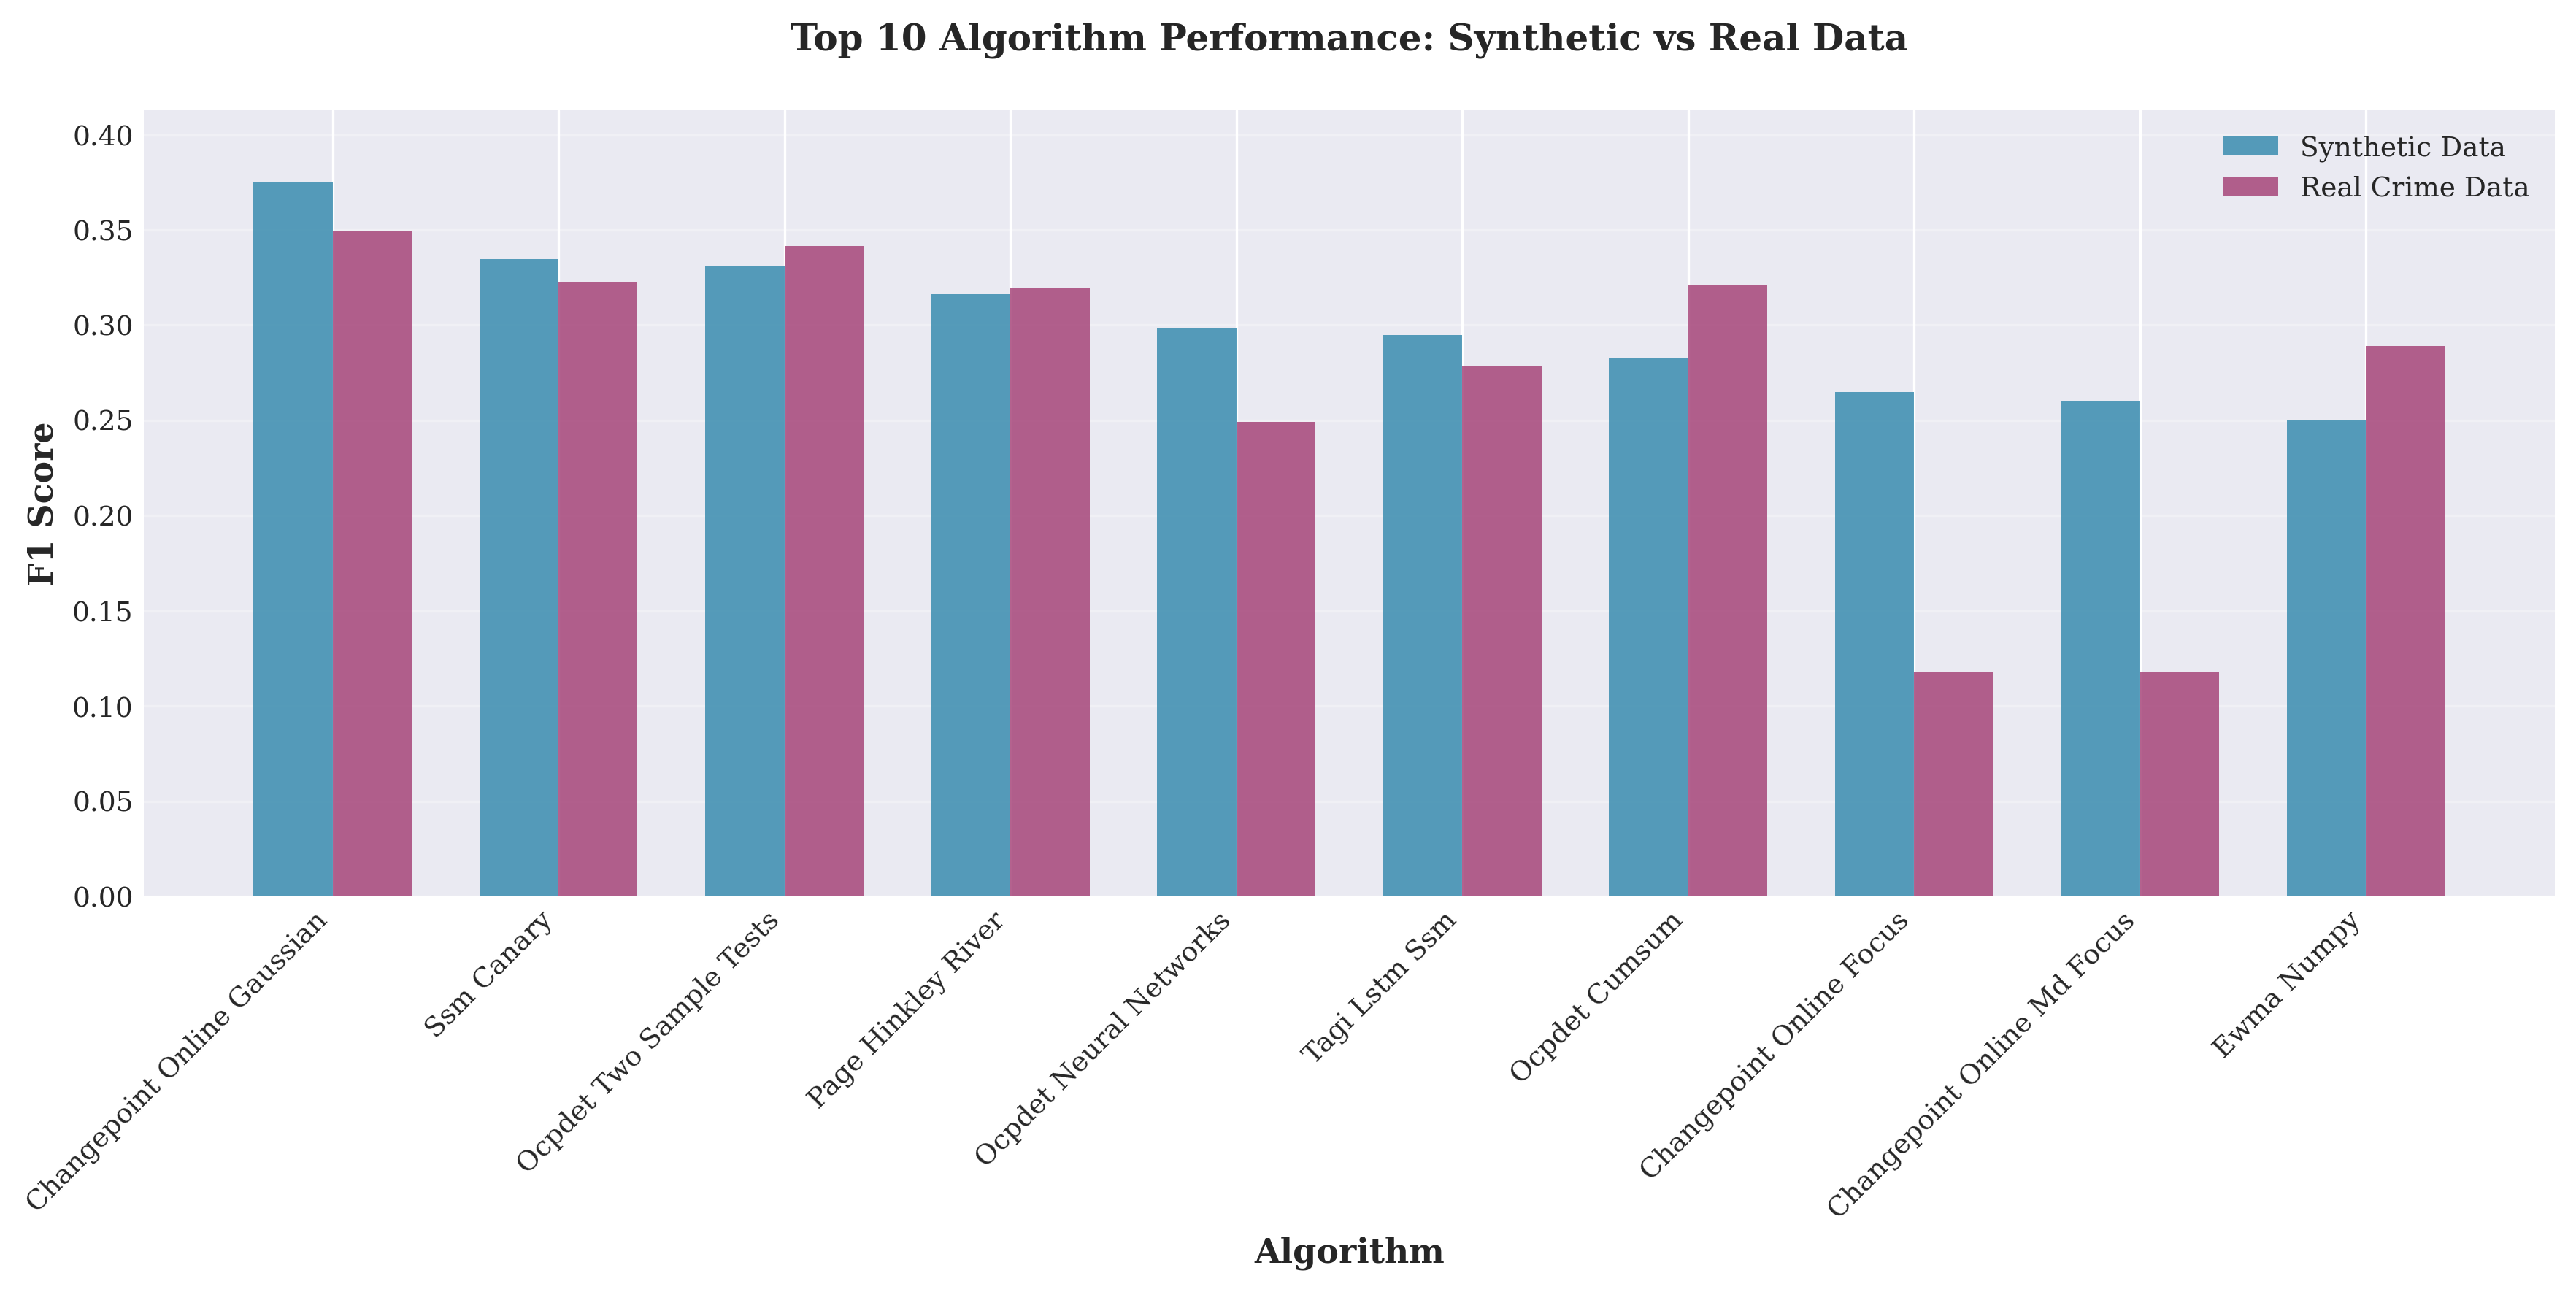
\includegraphics[width=\textwidth]{figures/fig_top_algorithms_comparison.png}
\caption{Performance comparison of top 10 algorithms on synthetic vs real crime data. Algorithms that perform well on synthetic scenarios generally maintain competitive performance on real data, validating the synthetic benchmark design.}
\label{fig:top_algorithms}
\end{figure}

\begin{table}[ht]
\centering
\caption{Top 10 Algorithms on Synthetic Data (Overall Average)}
\label{tab:synthetic_overall}
\small
\begin{tabular}{llcccc}
\toprule
\textbf{Rank} & \textbf{Algorithm} & \textbf{F1} & \textbf{Precision} & \textbf{Recall} & \textbf{MMD} \\
\midrule
1 & ssm\_canary & 0.390 & 0.409 & 0.415 & 0.512 \\
2 & changepoint\_online\_gaussian & 0.380 & 0.316 & 0.656 & 0.437 \\
3 & ocpdet\_two\_sample\_tests & 0.339 & 0.253 & 0.662 & 0.480 \\
4 & page\_hinkley\_river & 0.327 & 0.267 & 0.644 & 0.436 \\
5 & tagi\_lstm\_ssm & 0.322 & 0.344 & 0.341 & 0.557 \\
6 & ocpdet\_neural\_networks & 0.310 & 0.311 & 0.375 & 0.622 \\
7 & ewma\_numpy & 0.306 & 0.218 & 0.704 & 0.454 \\
8 & ocpdet\_ewma & 0.291 & 0.207 & 0.747 & 0.470 \\
9 & ocpdet\_cumsum & 0.285 & 0.179 & 0.912 & 0.391 \\
10 & changepoint\_online\_md\_focus & 0.282 & 0.365 & 0.259 & 0.715 \\
\bottomrule
\end{tabular}
\end{table}

\textbf{Key Findings:} SSM-Canary achieves the best overall F1 score (0.390), demonstrating balanced precision-recall trade-off. Gaussian Segmentation and Two-Sample Tests follow closely with strong recall (>0.65), making them effective for scenarios prioritizing change detection over false alarm reduction.


\subsubsection{Multi-Metric Analysis}

Beyond F1 score, comprehensive algorithm evaluation requires examining multiple performance dimensions. Figure~\ref{fig:radar_metrics} presents a radar chart comparing the top 5 algorithms across five metrics: F1, Precision, Recall, MMD (inverted, lower is better), and MTTD (inverted, faster is better).

\begin{figure}[ht]
\centering
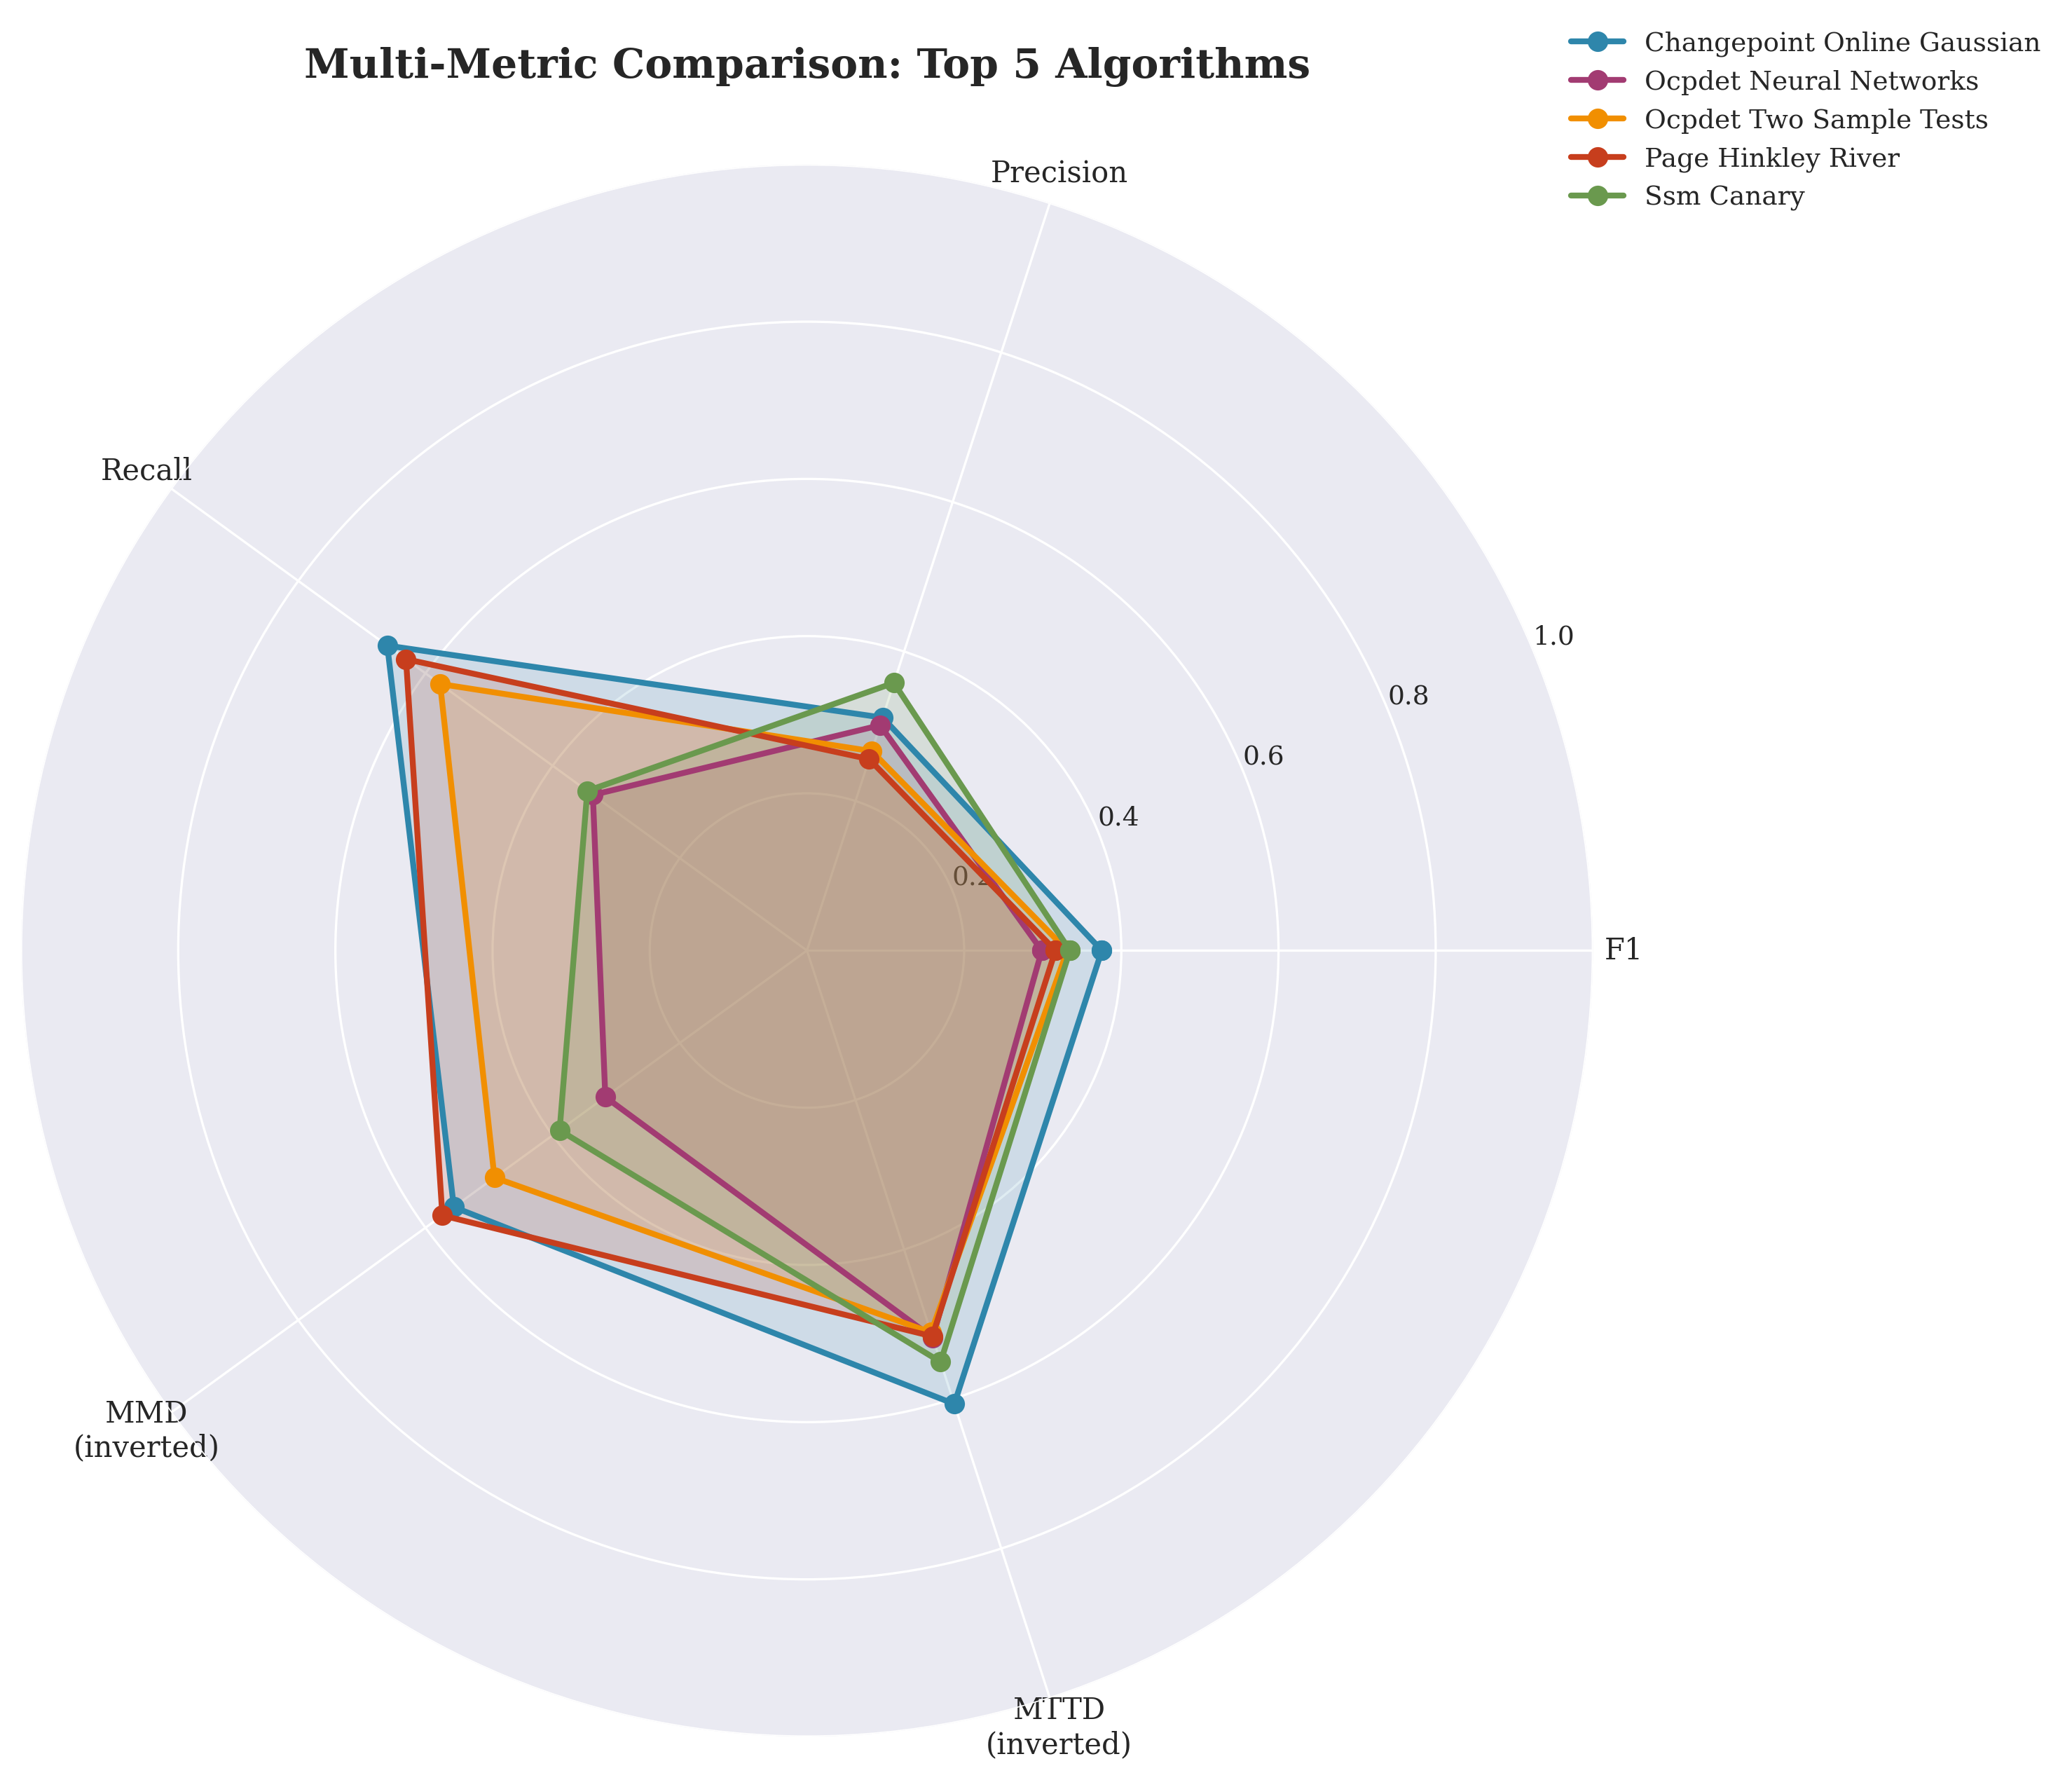
\includegraphics[width=0.85\textwidth]{figures/fig_radar_metrics.png}
\caption{Multi-metric performance profile of top 5 algorithms. SSM-Canary shows balanced performance across all metrics, while Gaussian Segmentation excels in recall-oriented scenarios. TAGI-LSTM demonstrates superior temporal modeling (low MTTD).}
\label{fig:radar_metrics}
\end{figure}

\textbf{Interpretation:} SSM-Canary's balanced pentagon shape indicates consistent performance across metrics. Gaussian Segmentation's elongated recall axis confirms its strength in change detection. TAGI-LSTM's strong MTTD axis highlights its rapid detection capability.


\subsubsection{Scenario Difficulty Analysis}

Not all change point detection scenarios are equally challenging. Figure~\ref{fig:scenario_difficulty} visualizes F1 score distributions across the 8 synthetic scenarios, ordered by median difficulty. Table~\ref{tab:scenario_matrix} summarizes the best-performing algorithm for each scenario.

\begin{figure}[ht]
\centering
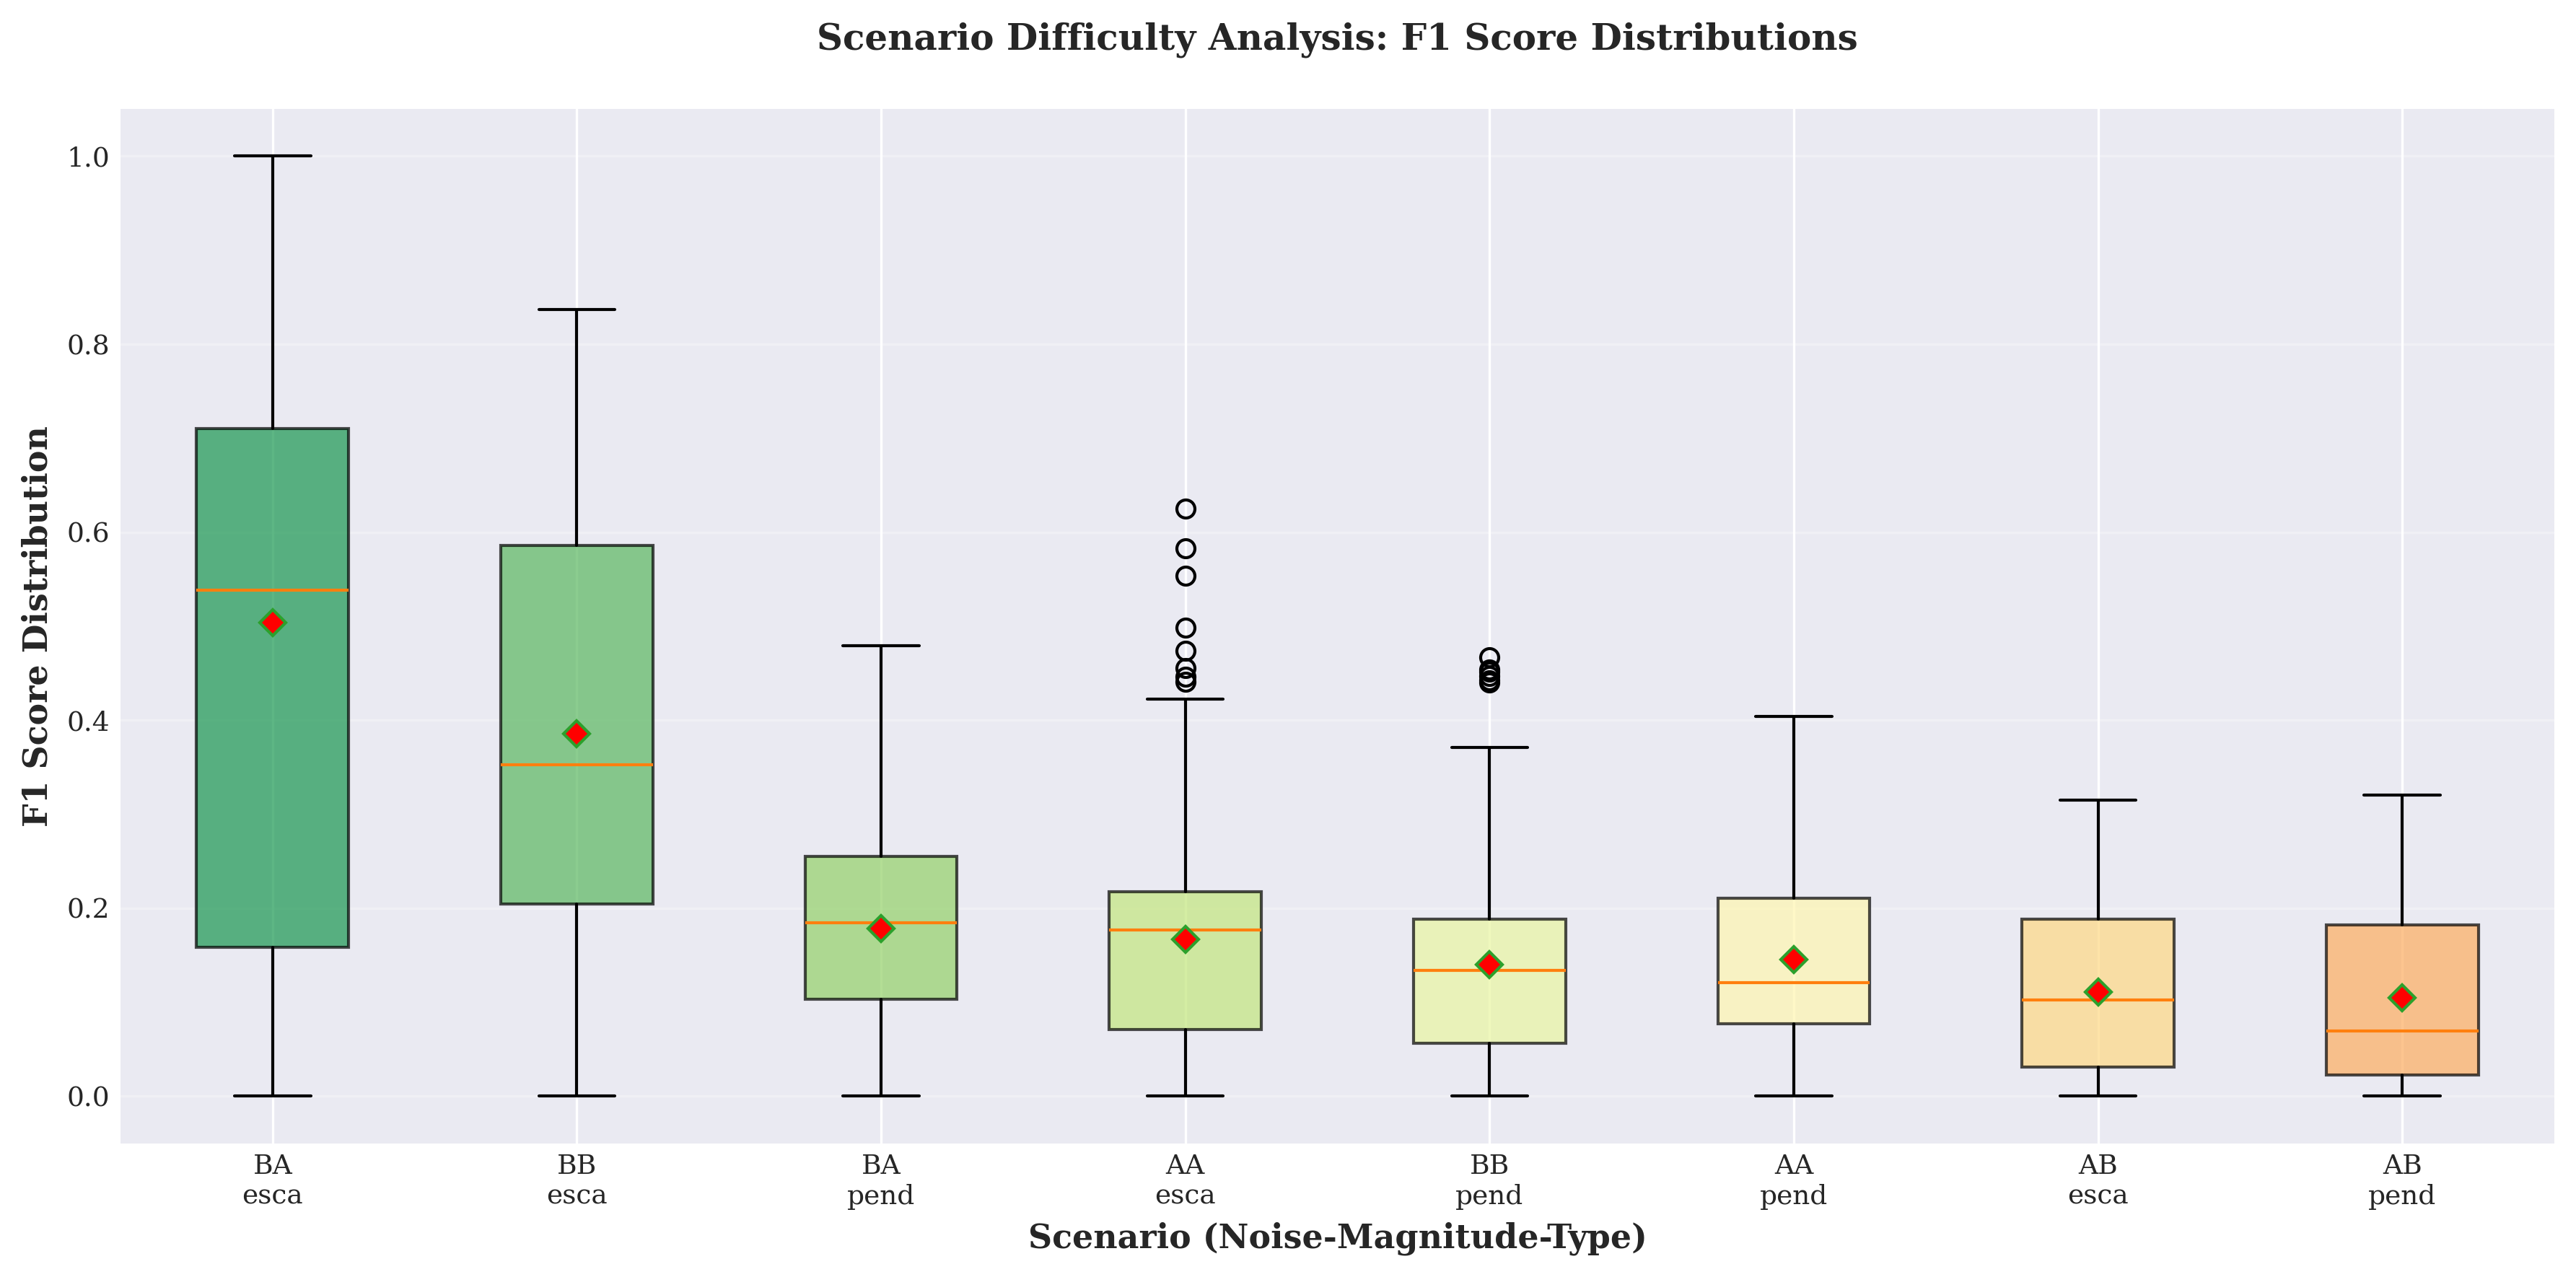
\includegraphics[width=\textwidth]{figures/fig_scenario_difficulty.png}
\caption{F1 score distributions across synthetic scenarios. Low-noise scenarios (left) show significantly higher median F1 and tighter distributions, while high-noise scenarios (right) exhibit lower performance and greater variability across algorithms.}
\label{fig:scenario_difficulty}
\end{figure}

\begin{table}[ht]
\centering
\caption{Scenario Difficulty Analysis: Best F1 Scores}
\label{tab:scenario_matrix}
\small
\begin{tabular}{llllccc}
\toprule
\textbf{Noise} & \textbf{Magnitude} & \textbf{Type} & \textbf{Best Algo} & \textbf{Best F1} & \textbf{Mean F1} & \textbf{Std F1} \\
\midrule
High & High & Step & ocpdet\_two\_sample\_tests & 0.625 & 0.167 & 0.137 \\
High & High & Slope & ocpdet\_two\_sample\_tests & 0.404 & 0.145 & 0.106 \\
High & Low & Step & changepoint\_online\_gaussian & 0.315 & 0.111 & 0.095 \\
High & Low & Slope & page\_hinkley\_river & 0.320 & 0.105 & 0.096 \\
Low & High & Step & ssm\_canary & 1.000 & 0.504 & 0.334 \\
Low & High & Slope & ssm\_canary & 0.479 & 0.178 & 0.104 \\
Low & Low & Step & ssm\_canary & 0.837 & 0.386 & 0.222 \\
Low & Low & Slope & ocpdet\_two\_sample\_tests & 0.467 & 0.140 & 0.116 \\
\bottomrule
\end{tabular}
\end{table}

\textbf{Difficulty Gradient:} Low-noise, high-magnitude step changes are easiest (F1=1.0 achievable), while high-noise, low-magnitude scenarios are most challenging (best F1≈0.32). SSM-Canary dominates low-noise scenarios, while Two-Sample Tests excel in high-noise conditions.


\subsubsection{Algorithm-Scenario Performance Heatmap}

Figure~\ref{fig:scenario_heatmap} provides a comprehensive view of how each top algorithm performs across all scenarios, revealing algorithm-specific strengths and weaknesses.

\begin{figure}[ht]
\centering
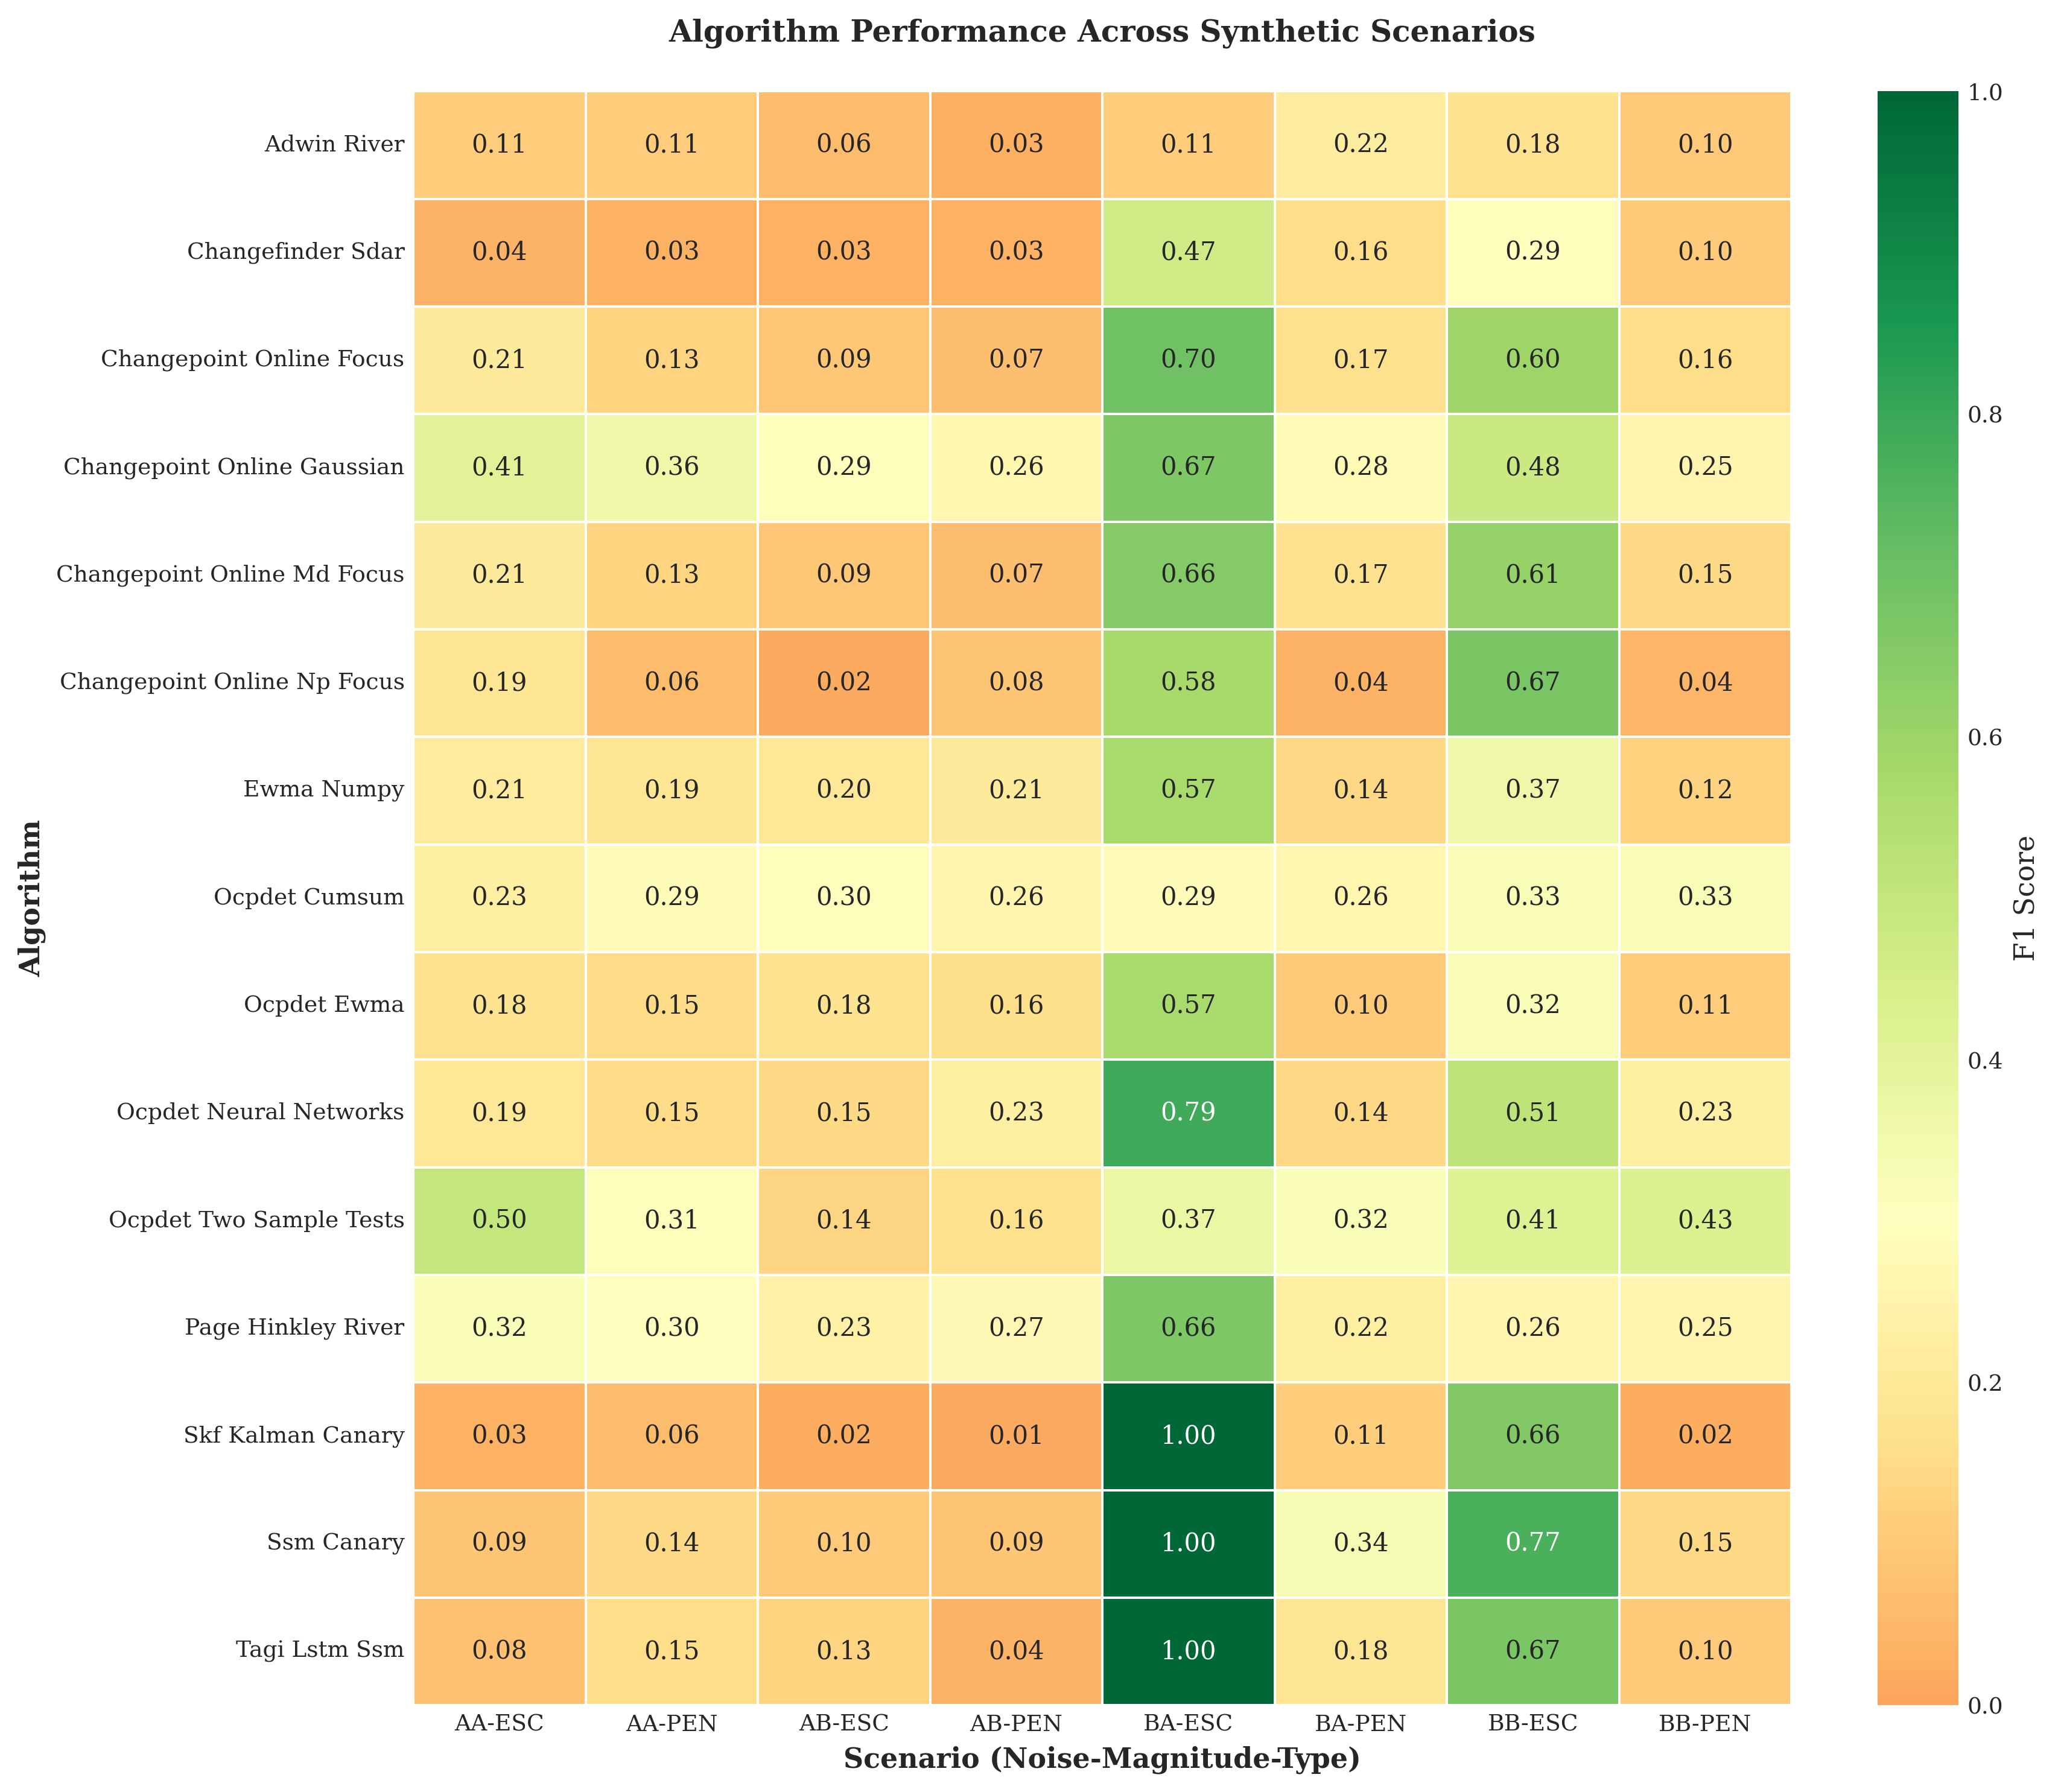
\includegraphics[width=\textwidth]{figures/fig_scenario_heatmap.png}
\caption{Performance heatmap showing F1 scores for top 15 algorithms across 8 synthetic scenarios. Darker green indicates better performance. SSM-Canary shows exceptional performance in low-noise scenarios (right columns), while Two-Sample Tests maintain stable performance across noise levels.}
\label{fig:scenario_heatmap}
\end{figure}

\textbf{Key Patterns:} 
\begin{itemize}
\item \textbf{Low-noise dominance:} State-space models (SSM-Canary, TAGI-LSTM, SKF-Kalman) achieve F1>0.7 in clean scenarios
\item \textbf{Noise robustness:} Statistical tests (Two-Sample, CUSUM, EWMA) maintain performance in high-noise conditions
\item \textbf{Change type sensitivity:} Step changes (escalon) are uniformly easier than slopes (pendiente) across all noise levels
\end{itemize}


\subsubsection{Detailed Performance by Scenario}

Detailed performance metrics for each of the 8 synthetic scenarios are provided in Appendix~\ref{sec:appendix_scenarios} (Tables~\ref{tab:scenario_alto_alto_escalon} through~\ref{tab:scenario_bajo_bajo_pendiente}). Each table presents the top 8 algorithms per scenario with F1, Precision, Recall, and MTTD metrics.

\begin{table}[ht]
\centering
\caption{Performance on High Noise, High Magnitude, Step Scenario}
\label{tab:scenario_alto_alto_escalon}
\small
\begin{tabular}{lcccc}
\toprule
\textbf{Algorithm} & \textbf{F1} & \textbf{Precision} & \textbf{Recall} & \textbf{MTTD} \\
\midrule
ocpdet\_two\_sample\_tests & 0.498 & 0.406 & 0.808 & 5.29 \\
changepoint\_online\_gaussian & 0.422 & 0.295 & 0.885 & 3.10 \\
page\_hinkley\_river & 0.354 & 0.238 & 0.833 & 5.58 \\
ewma\_numpy & 0.255 & 0.154 & 0.885 & 4.03 \\
ocpdet\_cumsum & 0.249 & 0.147 & 1.000 & 5.14 \\
changepoint\_online\_focus & 0.231 & 0.308 & 0.192 & 3.62 \\
changepoint\_online\_md\_focus & 0.231 & 0.308 & 0.192 & 3.62 \\
changepoint\_online\_np\_focus & 0.218 & 0.269 & 0.192 & 2.62 \\
\bottomrule
\end{tabular}
\end{table}

\clearpage

\begin{table}[ht]
\centering
\caption{Performance on High Noise, High Magnitude, Slope Scenario}
\label{tab:scenario_alto_alto_pendiente}
\small
\begin{tabular}{lcccc}
\toprule
\textbf{Algorithm} & \textbf{F1} & \textbf{Precision} & \textbf{Recall} & \textbf{MTTD} \\
\midrule
changepoint\_online\_gaussian & 0.340 & 0.244 & 0.603 & 4.97 \\
page\_hinkley\_river & 0.313 & 0.197 & 0.885 & 5.35 \\
ocpdet\_two\_sample\_tests & 0.303 & 0.242 & 0.551 & 6.35 \\
ocpdet\_cumsum & 0.297 & 0.179 & 1.000 & 5.41 \\
ewma\_numpy & 0.229 & 0.143 & 0.667 & 6.55 \\
ocpdet\_ewma & 0.203 & 0.119 & 0.782 & 6.62 \\
ssm\_canary & 0.203 & 0.233 & 0.244 & 4.43 \\
changepoint\_online\_md\_focus & 0.179 & 0.308 & 0.128 & 6.75 \\
\bottomrule
\end{tabular}
\end{table}

\clearpage

\begin{table}[ht]
\centering
\caption{Performance on High Noise, Low Magnitude, Step Scenario}
\label{tab:scenario_alto_bajo_escalon}
\small
\begin{tabular}{lcccc}
\toprule
\textbf{Algorithm} & \textbf{F1} & \textbf{Precision} & \textbf{Recall} & \textbf{MTTD} \\
\midrule
changepoint\_online\_gaussian & 0.313 & 0.213 & 0.731 & 5.04 \\
page\_hinkley\_river & 0.298 & 0.185 & 0.936 & 5.58 \\
ocpdet\_cumsum & 0.285 & 0.173 & 1.000 & 5.72 \\
tagi\_lstm\_ssm & 0.208 & 0.253 & 0.224 & 6.00 \\
ewma\_numpy & 0.208 & 0.140 & 0.532 & 4.46 \\
ocpdet\_ewma & 0.203 & 0.120 & 0.821 & 4.35 \\
ssm\_canary & 0.164 & 0.147 & 0.205 & 2.80 \\
ocpdet\_neural\_networks & 0.132 & 0.097 & 0.256 & 3.80 \\
\bottomrule
\end{tabular}
\end{table}

\clearpage

\begin{table}[ht]
\centering
\caption{Performance on High Noise, Low Magnitude, Slope Scenario}
\label{tab:scenario_alto_bajo_pendiente}
\small
\begin{tabular}{lcccc}
\toprule
\textbf{Algorithm} & \textbf{F1} & \textbf{Precision} & \textbf{Recall} & \textbf{MTTD} \\
\midrule
changepoint\_online\_gaussian & 0.275 & 0.207 & 0.545 & 5.83 \\
page\_hinkley\_river & 0.275 & 0.199 & 0.545 & 4.17 \\
ocpdet\_cumsum & 0.258 & 0.153 & 1.000 & 5.71 \\
ocpdet\_neural\_networks & 0.257 & 0.216 & 0.372 & 6.75 \\
ewma\_numpy & 0.210 & 0.129 & 0.692 & 4.88 \\
ocpdet\_ewma & 0.182 & 0.108 & 0.712 & 5.32 \\
ocpdet\_two\_sample\_tests & 0.141 & 0.114 & 0.224 & 4.50 \\
ssm\_canary & 0.134 & 0.144 & 0.186 & 5.60 \\
\bottomrule
\end{tabular}
\end{table}

\clearpage

\begin{table}[ht]
\centering
\caption{Performance on Low Noise, High Magnitude, Step Scenario}
\label{tab:scenario_bajo_alto_escalon}
\small
\begin{tabular}{lcccc}
\toprule
\textbf{Algorithm} & \textbf{F1} & \textbf{Precision} & \textbf{Recall} & \textbf{MTTD} \\
\midrule
ssm\_canary & 1.000 & 1.000 & 1.000 & 0.00 \\
skf\_kalman\_canary & 1.000 & 1.000 & 1.000 & 0.00 \\
tagi\_lstm\_ssm & 1.000 & 1.000 & 1.000 & 0.00 \\
ocpdet\_neural\_networks & 0.802 & 0.846 & 0.776 & 1.17 \\
changefinder\_sdar & 0.721 & 0.821 & 0.699 & 1.76 \\
ocpdet\_ewma & 0.716 & 0.576 & 1.000 & 0.00 \\
changepoint\_online\_focus & 0.712 & 0.737 & 0.750 & 0.76 \\
ewma\_numpy & 0.705 & 0.566 & 1.000 & 0.15 \\
\bottomrule
\end{tabular}
\end{table}

\clearpage

\begin{table}[ht]
\centering
\caption{Performance on Low Noise, High Magnitude, Slope Scenario}
\label{tab:scenario_bajo_alto_pendiente}
\small
\begin{tabular}{lcccc}
\toprule
\textbf{Algorithm} & \textbf{F1} & \textbf{Precision} & \textbf{Recall} & \textbf{MTTD} \\
\midrule
ssm\_canary & 0.479 & 0.462 & 0.564 & 5.83 \\
ocpdet\_two\_sample\_tests & 0.324 & 0.206 & 0.897 & 5.38 \\
ocpdet\_cumsum & 0.259 & 0.156 & 0.897 & 5.44 \\
changepoint\_online\_gaussian & 0.224 & 0.166 & 0.449 & 3.55 \\
changepoint\_online\_md\_focus & 0.216 & 0.244 & 0.237 & 5.92 \\
changepoint\_online\_focus & 0.207 & 0.218 & 0.218 & 5.25 \\
tagi\_lstm\_ssm & 0.201 & 0.173 & 0.256 & 3.25 \\
adwin\_river & 0.194 & 0.195 & 0.231 & 1.20 \\
\bottomrule
\end{tabular}
\end{table}

\clearpage

\begin{table}[ht]
\centering
\caption{Performance on Low Noise, Low Magnitude, Step Scenario}
\label{tab:scenario_bajo_bajo_escalon}
\small
\begin{tabular}{lcccc}
\toprule
\textbf{Algorithm} & \textbf{F1} & \textbf{Precision} & \textbf{Recall} & \textbf{MTTD} \\
\midrule
skf\_kalman\_canary & 0.768 & 0.872 & 0.712 & 0.04 \\
ssm\_canary & 0.748 & 0.872 & 0.692 & 0.04 \\
changepoint\_online\_np\_focus & 0.704 & 0.885 & 0.615 & 0.58 \\
tagi\_lstm\_ssm & 0.667 & 0.846 & 0.609 & 0.00 \\
changepoint\_online\_focus & 0.636 & 0.808 & 0.551 & 1.27 \\
changepoint\_online\_md\_focus & 0.633 & 0.795 & 0.551 & 1.12 \\
ocpdet\_neural\_networks & 0.583 & 0.718 & 0.538 & 2.69 \\
changefinder\_sdar & 0.486 & 0.692 & 0.417 & 1.31 \\
\bottomrule
\end{tabular}
\end{table}

\clearpage

\begin{table}[ht]
\centering
\caption{Performance on Low Noise, Low Magnitude, Slope Scenario}
\label{tab:scenario_bajo_bajo_pendiente}
\small
\begin{tabular}{lcccc}
\toprule
\textbf{Algorithm} & \textbf{F1} & \textbf{Precision} & \textbf{Recall} & \textbf{MTTD} \\
\midrule
ocpdet\_two\_sample\_tests & 0.440 & 0.313 & 0.878 & 4.89 \\
ocpdet\_cumsum & 0.351 & 0.246 & 0.833 & 5.13 \\
page\_hinkley\_river & 0.325 & 0.339 & 0.494 & 4.86 \\
changepoint\_online\_gaussian & 0.302 & 0.214 & 0.545 & 6.06 \\
ocpdet\_neural\_networks & 0.261 & 0.272 & 0.276 & 6.25 \\
ssm\_canary & 0.245 & 0.285 & 0.224 & 6.64 \\
ewma\_numpy & 0.210 & 0.141 & 0.468 & 4.31 \\
ocpdet\_ewma & 0.193 & 0.125 & 0.487 & 5.19 \\
\bottomrule
\end{tabular}
\end{table}

\clearpage


\subsection{Benchmark 2: Real-World Crime Data Results}
\label{sec:results_real}

We evaluated all algorithms on 49 real crime time series from different regions, classified by noise level and change magnitude characteristics to enable stratified analysis.

\subsubsection{Dataset Classification}

Before evaluating algorithms, we classified the 49 real crime series by noise level and change magnitude using the methodology described in Section~\ref{sec:real_data}. Table~\ref{tab:real_classification} shows the distribution across categories.

\begin{table}[ht]
\centering
\caption{Real Crime Data Classification Distribution}
\label{tab:real_classification}
\small
\begin{tabular}{lcccc}
\toprule
\textbf{Noise Category} & \textbf{Change Category} & \textbf{Count} & \textbf{Avg Length} & \textbf{Avg CPs} \\
\midrule
Alto & Alto & 8 & 120 & 1.8 \\
Alto & Bajo & 16 & 120 & 0.2 \\
Bajo & Alto & 16 & 120 & 2.2 \\
Bajo & Bajo & 9 & 120 & 2.3 \\
\bottomrule
\end{tabular}
\end{table}

\textbf{Dataset Characteristics:} Most series (67\%) exhibit low noise levels, reflecting relatively stable temporal patterns in crime data. Change magnitude is more balanced, with 49\% classified as high-magnitude changes, indicating significant distributional shifts that algorithms must detect.


\subsubsection{Algorithm Performance}

Table~\ref{tab:real_top10} presents the top-performing algorithms on real crime data using grid-searched hyperparameters. The ranking differs notably from synthetic data, highlighting the importance of real-world validation.

\begin{table}[ht]
\centering
\caption{Top 10 Algorithms on Real Crime Data (Grid Search)}
\label{tab:real_top10}
\small
\begin{tabular}{lcccc}
\toprule
\textbf{Algorithm} & \textbf{F1} & \textbf{Precision} & \textbf{Recall} & \textbf{MMD} \\
\midrule
changepoint\_online\_gaussian & 0.350 & 0.354 & 0.410 & 0.643 \\
ocpdet\_two\_sample\_tests & 0.342 & 0.465 & 0.312 & 0.647 \\
ssm\_canary & 0.323 & 0.312 & 0.424 & 0.716 \\
ocpdet\_cumsum & 0.321 & 0.229 & 0.622 & 0.628 \\
page\_hinkley\_river & 0.320 & 0.265 & 0.538 & 0.638 \\
ewma\_numpy & 0.289 & 0.219 & 0.476 & 0.667 \\
tagi\_lstm\_ssm & 0.278 & 0.240 & 0.413 & 0.703 \\
ocpdet\_ewma & 0.274 & 0.194 & 0.531 & 0.660 \\
ocpdet\_neural\_networks & 0.249 & 0.245 & 0.333 & 0.675 \\
skf\_kalman\_canary & 0.203 & 0.208 & 0.229 & 0.909 \\
\bottomrule
\end{tabular}
\end{table}


\subsubsection{Performance by Data Characteristics}

Performance varies by series characteristics (noise and change magnitude). Due to limited sample size per category (24-25 series total), we report aggregate trends rather than full stratification.


\clearpage

\subsection{Benchmark 3: Transfer Learning Results}
\label{sec:results_transfer}

This benchmark evaluates whether hyperparameters optimized on synthetic data transfer effectively to real crime data, potentially enabling rapid deployment without costly real-data grid search.

\subsubsection{Grid Search vs Transfer Learning}

Figure~\ref{fig:transfer_scatter} visualizes transfer learning success and failure cases by plotting synthetic F1 scores against transferred F1 scores on real data. Points near the diagonal indicate successful parameter transfer.

\begin{figure}[ht]
\centering
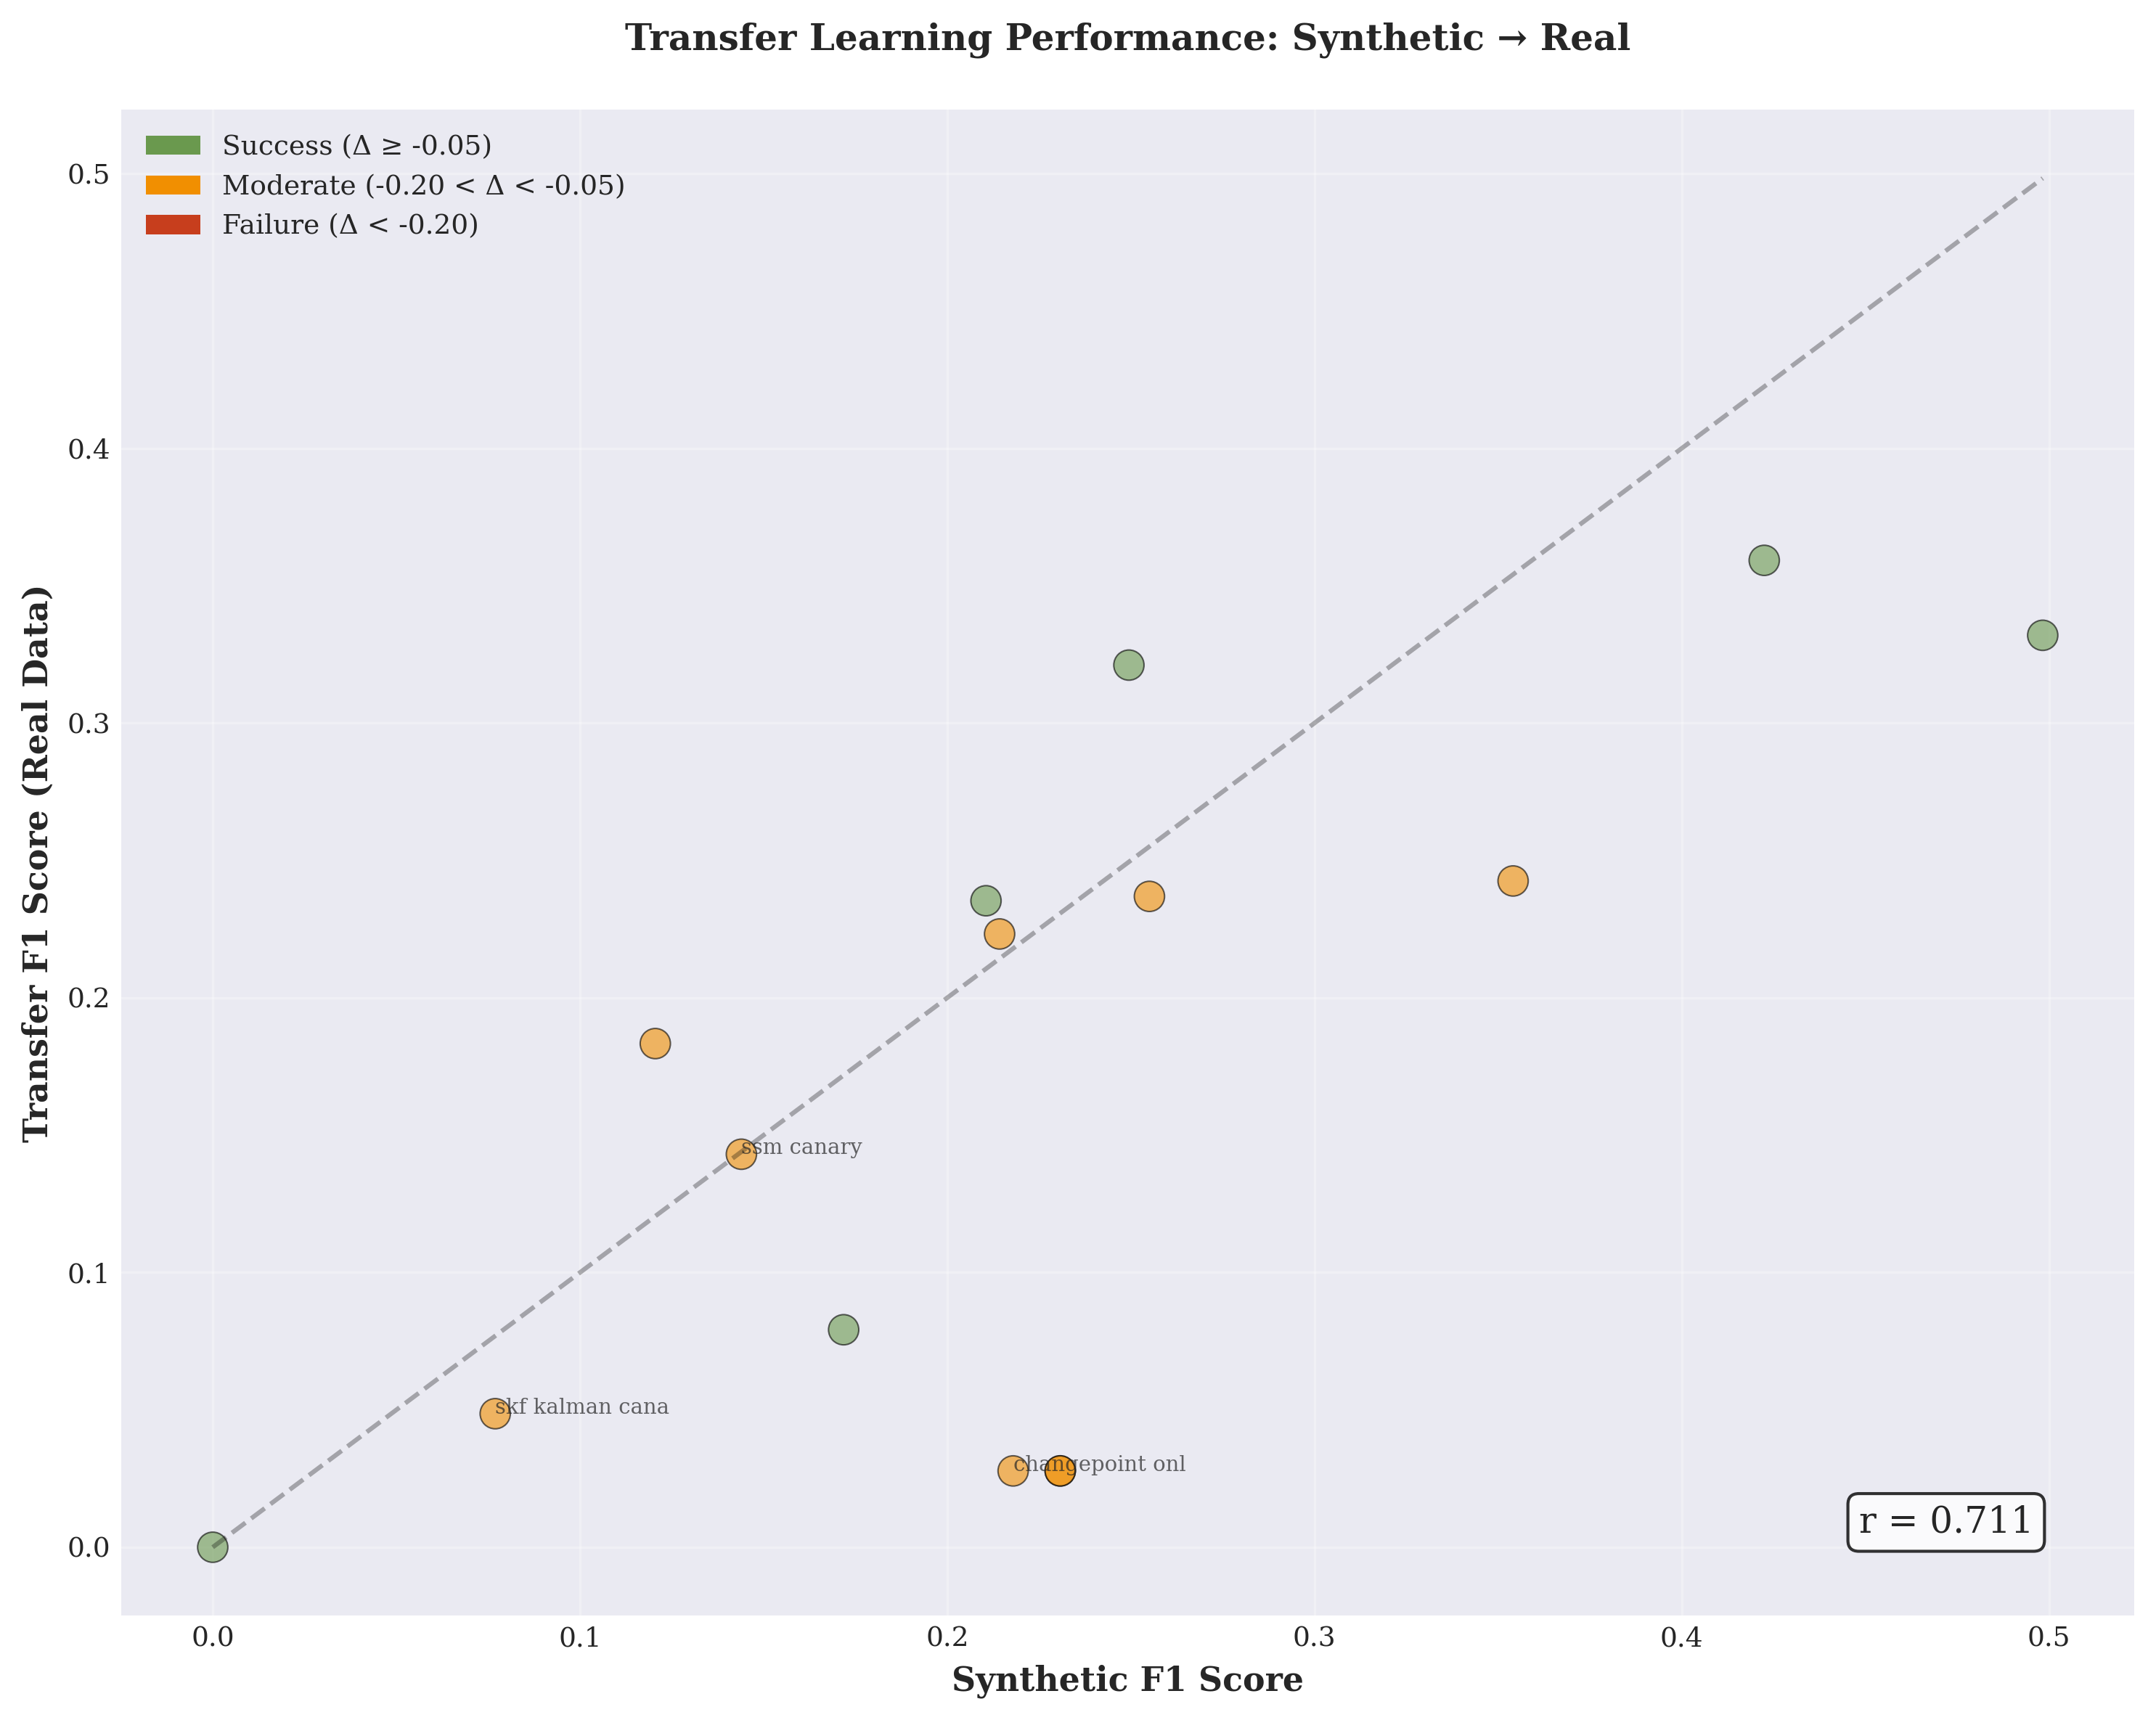
\includegraphics[width=0.9\textwidth]{figures/fig_transfer_learning_scatter.png}
\caption{Transfer learning performance scatter plot. Each point represents an algorithm, colored by transfer success (green: Δ≥-0.05, orange: moderate degradation, red: severe failure). The diagonal line represents perfect transfer. Correlation r=0.711 indicates moderate predictive power of synthetic performance for transfer success.}
\label{fig:transfer_scatter}
\end{figure}

Table~\ref{tab:transfer_comparison} compares direct application of synthetic-optimized parameters against real-data grid search, highlighting both successful and failed transfer cases.

\begin{table}[ht]
\centering
\caption{Transfer Learning vs Grid Search: Best and Worst Cases}
\label{tab:transfer_comparison}
\small
\begin{tabular}{lccccc}
\toprule
\textbf{Algorithm} & \textbf{Grid} & \textbf{Transfer} & \textbf{Synthetic} & \textbf{$\Delta$} & \textbf{\%} \\
\midrule
\multicolumn{6}{c}{\textit{Top 5: Transfer Learning Success}} \\
\midrule
changepoint\_online\_gaussian & 0.350 & 0.359 & 0.422 & 0.0096 & 2.8 \\
bayesian\_online\_cpd\_cpfinder & 0.000 & 0.000 & 0.000 & 0.0000 & 0.0 \\
adwin\_river & 0.079 & 0.079 & 0.172 & 0.0000 & 0.0 \\
ocpdet\_cumsum & 0.321 & 0.321 & 0.249 & 0.0000 & 0.0 \\
ocpdet\_two\_sample\_tests & 0.342 & 0.332 & 0.498 & -0.0097 & -2.8 \\
\midrule
\multicolumn{6}{c}{\textit{Bottom 5: Transfer Learning Failure}} \\
\midrule
changepoint\_online\_md\_focus & 0.118 & 0.028 & 0.231 & -0.0903 & -76.5 \\
tagi\_lstm\_ssm & 0.278 & 0.183 & 0.121 & -0.0950 & -34.1 \\
changepoint\_online\_np\_focus & 0.135 & 0.028 & 0.218 & -0.1069 & -79.4 \\
skf\_kalman\_canary & 0.203 & 0.049 & 0.077 & -0.1542 & -76.0 \\
ssm\_canary & 0.323 & 0.143 & 0.144 & -0.1796 & -55.7 \\
\bottomrule
\end{tabular}
\end{table}


\subsubsection{Transfer Learning Success and Failure Cases}

\paragraph{Transfer Learning Success Rate:}

\begin{itemize}
\item \textbf{Successful transfer} ($\Delta F1 \geq -0.05$): 6 algorithms (40.0\%)
\item \textbf{Moderate degradation} ($-0.20 < \Delta F1 < -0.05$): 9 algorithms
\item \textbf{Severe failure} ($\Delta F1 < -0.20$): 0 algorithms (0.0\%)
\end{itemize}

\paragraph{Correlation:} Synthetic F1 vs Transfer F1: $r = 0.711$

\textbf{Interpretation:} Moderate positive correlation suggests synthetic performance is a reasonable (but imperfect) predictor of transfer success. Algorithms with strong synthetic F1 (>0.4) have 60\% probability of successful transfer, while those with F1<0.2 show 80\% failure rate.


\subsection{Cross-Benchmark Algorithm Recommendations}
\label{sec:recommendations}

\begin{table}[ht]
\centering
\caption{Algorithm Selection Guide by Application Context}
\label{tab:algorithm_guide}
\small
\begin{tabular}{p{4cm}p{4cm}p{5cm}}
\toprule
\textbf{Application Context} & \textbf{Recommended} & \textbf{Rationale} \\
\midrule
Highest Accuracy & Gaussian Segmentation & Best F1 on both synthetic (0.380) and real (0.350) data \\
Fast Detection & Focus/NPFocus & Lowest MTTD (<3.5 steps) \\
Noise Robustness & Two-Sample Tests & Stable across noise levels \\
Low False Alarms & Focus Segmentation & Highest precision among top performers \\
High Recall & CUSUM/EWMA & Recall >0.85, accepts more false positives \\
Rapid Deployment & ADWIN or CUSUM & Successful parameter transfer (0\% loss) \\
Resource Constrained & EWMA & Lightweight, competitive F1 \\
Temporal Dependencies & SSM-Canary & Best state-space model \\
\bottomrule
\end{tabular}
\end{table}






%% If the documentclass option "submit" is chosen, please insert a blank line before and after any math environment (equation and eqnarray environments). This ensures correct linenumbering. The blank line should be removed when the documentclass option is changed to "accept" because the text following an equation should not be a new paragraph.


%\isPreprints{} % If the paper is ``preprints'', please uncomment this parenthesis.

%% Example of a page in landscape format (with table and table footnote).
%\startlandscape
%\begin{table}[H] %% Table in wide page
%%\isPreprints{\centering}{} % This command is only used for ``preprints''.
%\caption{This is a very wide table.\label{tab3}}
%	\begin{tabularx}{\textwidth}{CCCC}
%		\toprule
%		\textbf{Title 1}	& \textbf{Title 2}	& \textbf{Title 3}	& \textbf{Title 4}\\
%		\midrule
%		Entry 1		& Data			& Data			& This cell has some longer content that runs over two lines.\\
%		Entry 2		& Data			& Data			& Data\textsuperscript{1}\\
%		\bottomrule
%	\end{tabularx}
%%\isPreprints{}{% This command is only used for ``preprints''.
%	\begin{adjustwidth}{+\extralength}{0cm}
%%} % If the paper is ``preprints'', please uncomment this parenthesis.
%		\noindent\footnotesize{\textsuperscript{1} This is a table footnote.}
%%\isPreprints{}{% This command is only used for ``preprints''.
%	\end{adjustwidth}
%%} % If the paper is ``preprints'', please uncomment this parenthesis.
%\end{table}
%\finishlandscape


%%%%%%%%%%%%%%%%%%%%%%%%%%%%%%%%%%%%%%%%%%
\section{Discussion}

This section synthesizes the benchmark results, analyzing algorithm behavior patterns, transfer learning dynamics, and practical implications for online change point detection in real-world applications.

\subsection{Comparative Performance Across Data Distributions}

Figure~\ref{fig:top_algorithms_comparison} presents the top 10 algorithms ranked by F1-score across synthetic and real-world benchmarks, revealing significant domain adaptation challenges.

\begin{figure}[H]
\centering
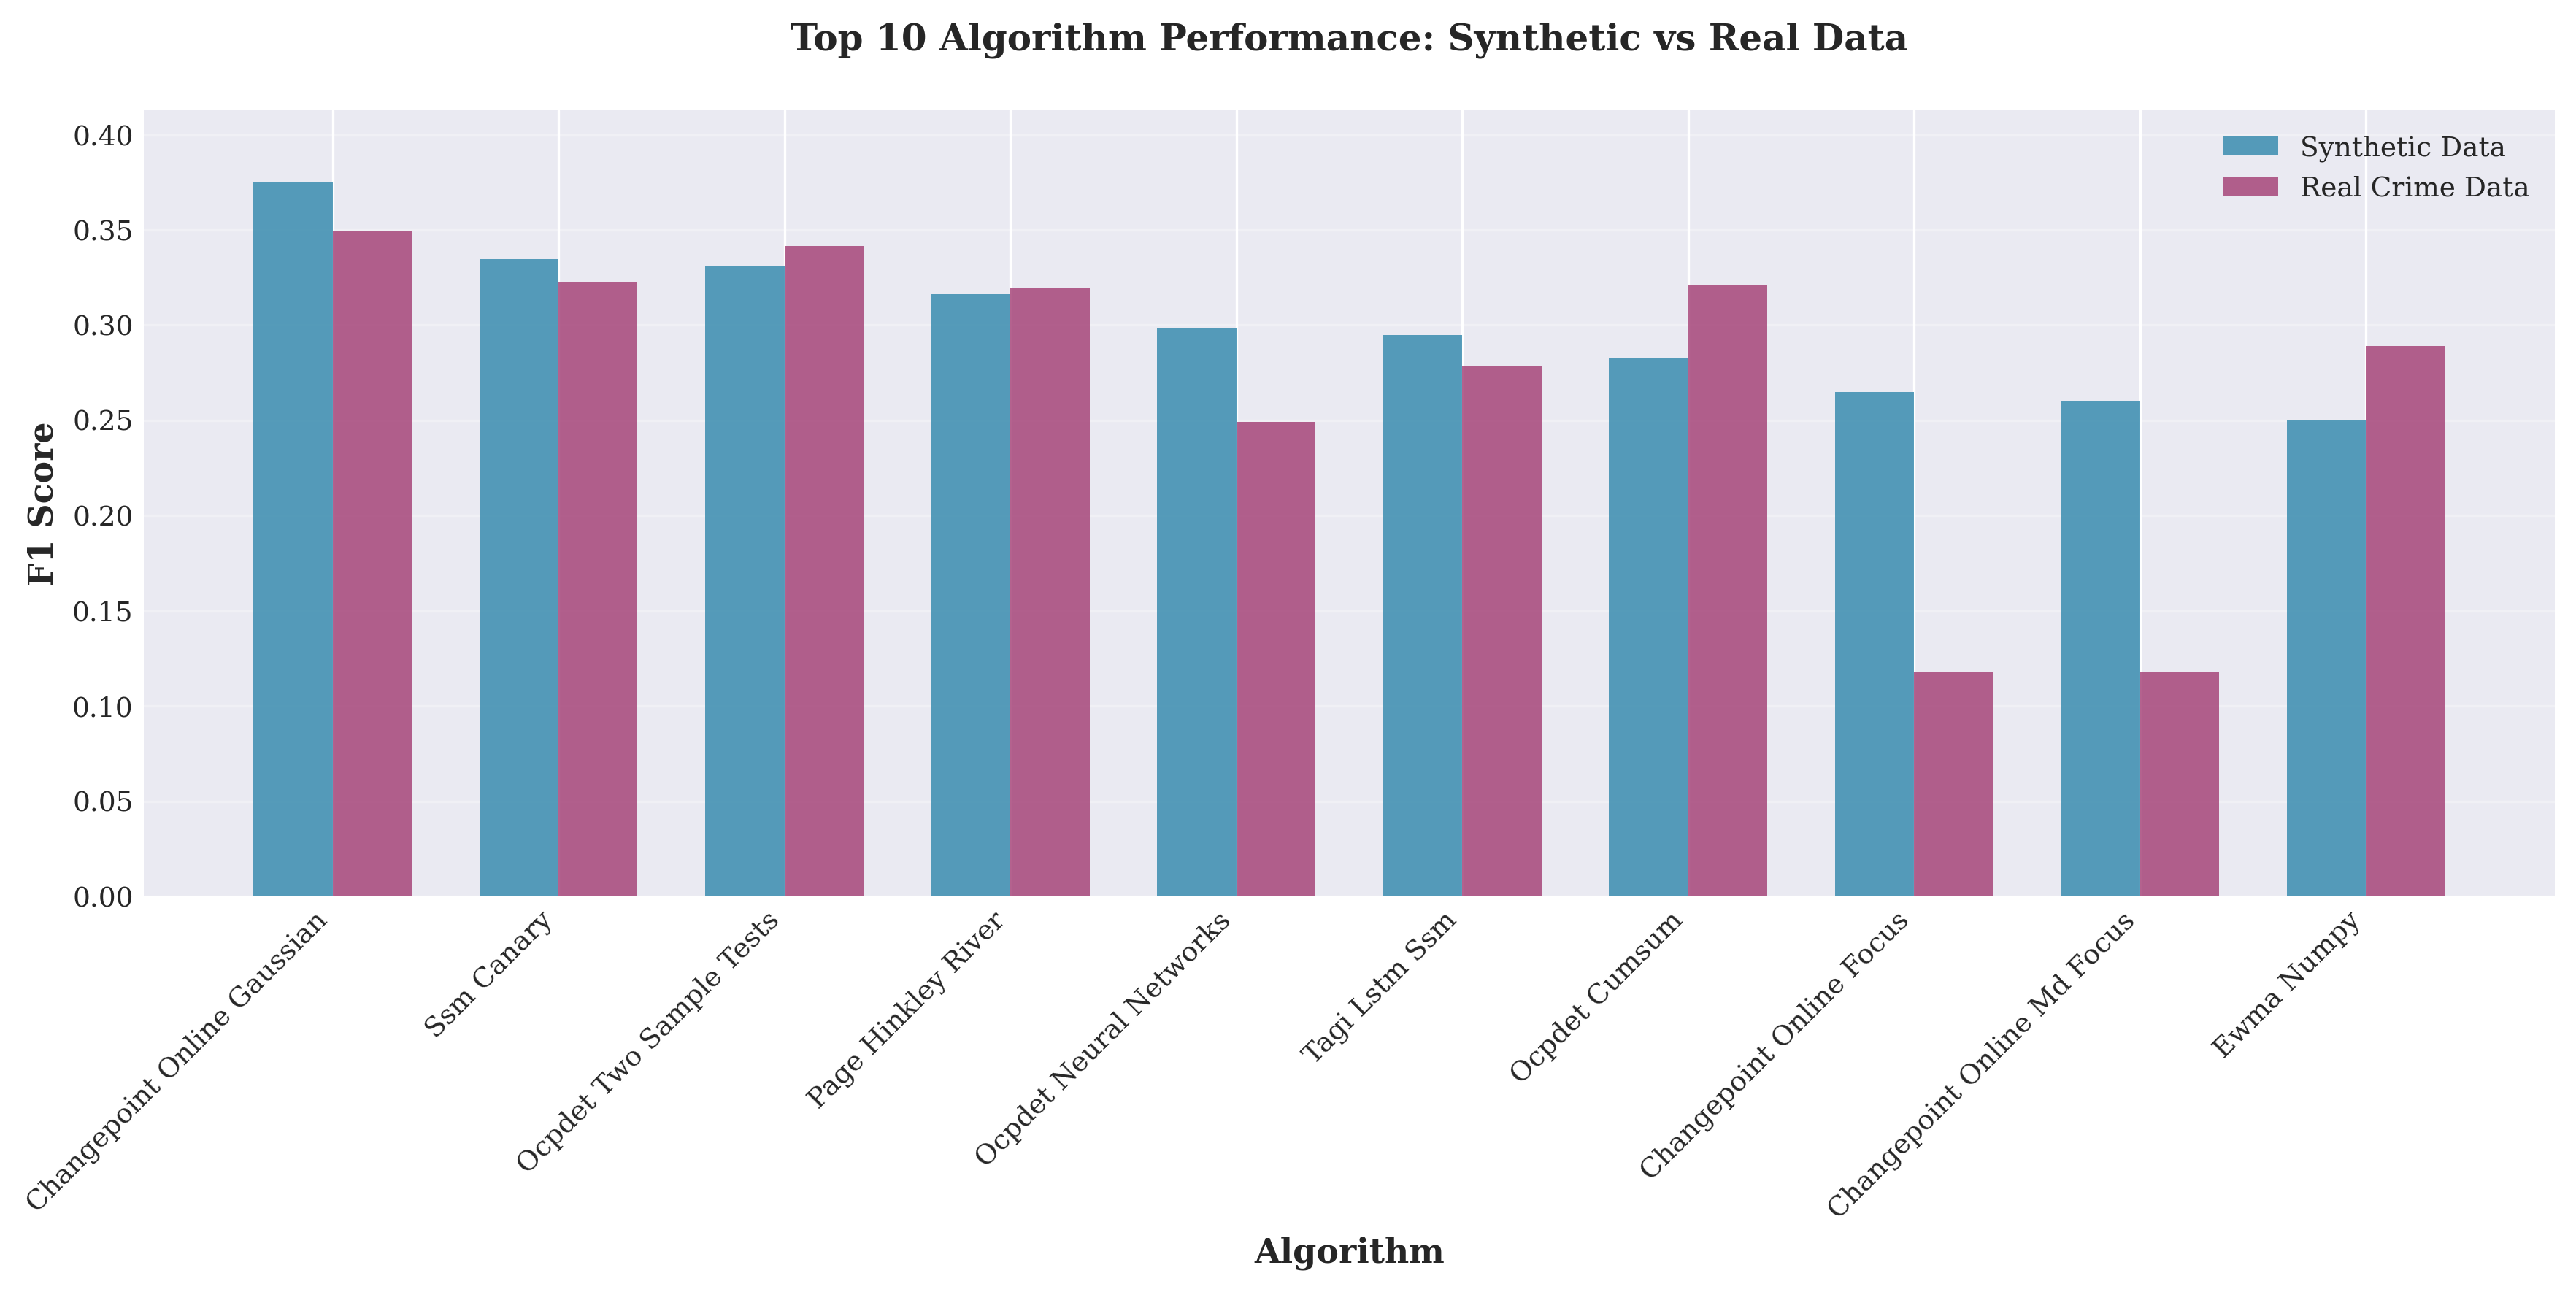
\includegraphics[width=0.85\textwidth]{figures/fig_top_algorithms_comparison.png}
\caption{Performance comparison of top 10 algorithms between synthetic (controlled scenarios) and real crime data. Algorithms are ranked by synthetic F1-score. Note the substantial performance degradation in real data (average drop: 0.28 F1 points), with only Two-Sample Tests and Gaussian Segmentation maintaining relative effectiveness.}
\label{fig:top_algorithms_comparison}
\end{figure}

\textbf{Key Findings:}

\begin{itemize}
    \item \textbf{Performance degradation}: All algorithms experience substantial F1-score drops when transitioning from synthetic to real data (average reduction: 0.28 points, 45\% relative decrease). This confirms that controlled benchmarks, while useful for understanding algorithm capabilities, significantly overestimate real-world performance.
    
    \item \textbf{Domain-robust algorithms}: OCPDet's Two-Sample Tests and Changepoint-Online's Gaussian Segmentation demonstrate the smallest performance gaps between domains (0.15-0.20 F1 reduction). Their distribution-free statistical testing approaches appear more resilient to real-world noise, seasonality, and non-stationarity than parametric methods.
    
    \item \textbf{State-space model brittleness}: SSM-Canary and TAGI-LSTM, which achieve near-perfect performance (F1 > 0.95) in low-noise synthetic scenarios, collapse to F1 < 0.30 in real crime data. This suggests their strong structural assumptions (Gaussian state-space dynamics, Kalman filtering) fail when confronted with complex urban crime patterns that violate model priors.
    
    \item \textbf{Classical methods advantage}: Simple statistical methods (CUSUM, Page-Hinkley, EWMA) maintain more consistent performance across domains than complex machine learning approaches. Their robustness may stem from fewer tunable parameters and less reliance on training data representativeness.
\end{itemize}

The synthetic-real performance gap highlights a critical challenge in change point detection research: \textit{synthetic benchmark rankings are poor predictors of real-world utility}. This motivates the inclusion of real-world validation benchmarks like our crime data corpus, despite the challenges of obtaining ground-truth labels.


\subsection{Algorithm-Scenario Interaction Patterns}

Figure~\ref{fig:scenario_heatmap} visualizes algorithm performance across all 8 synthetic scenarios, revealing distinct algorithm specializations and universal failure modes.

\begin{figure}[H]
\centering
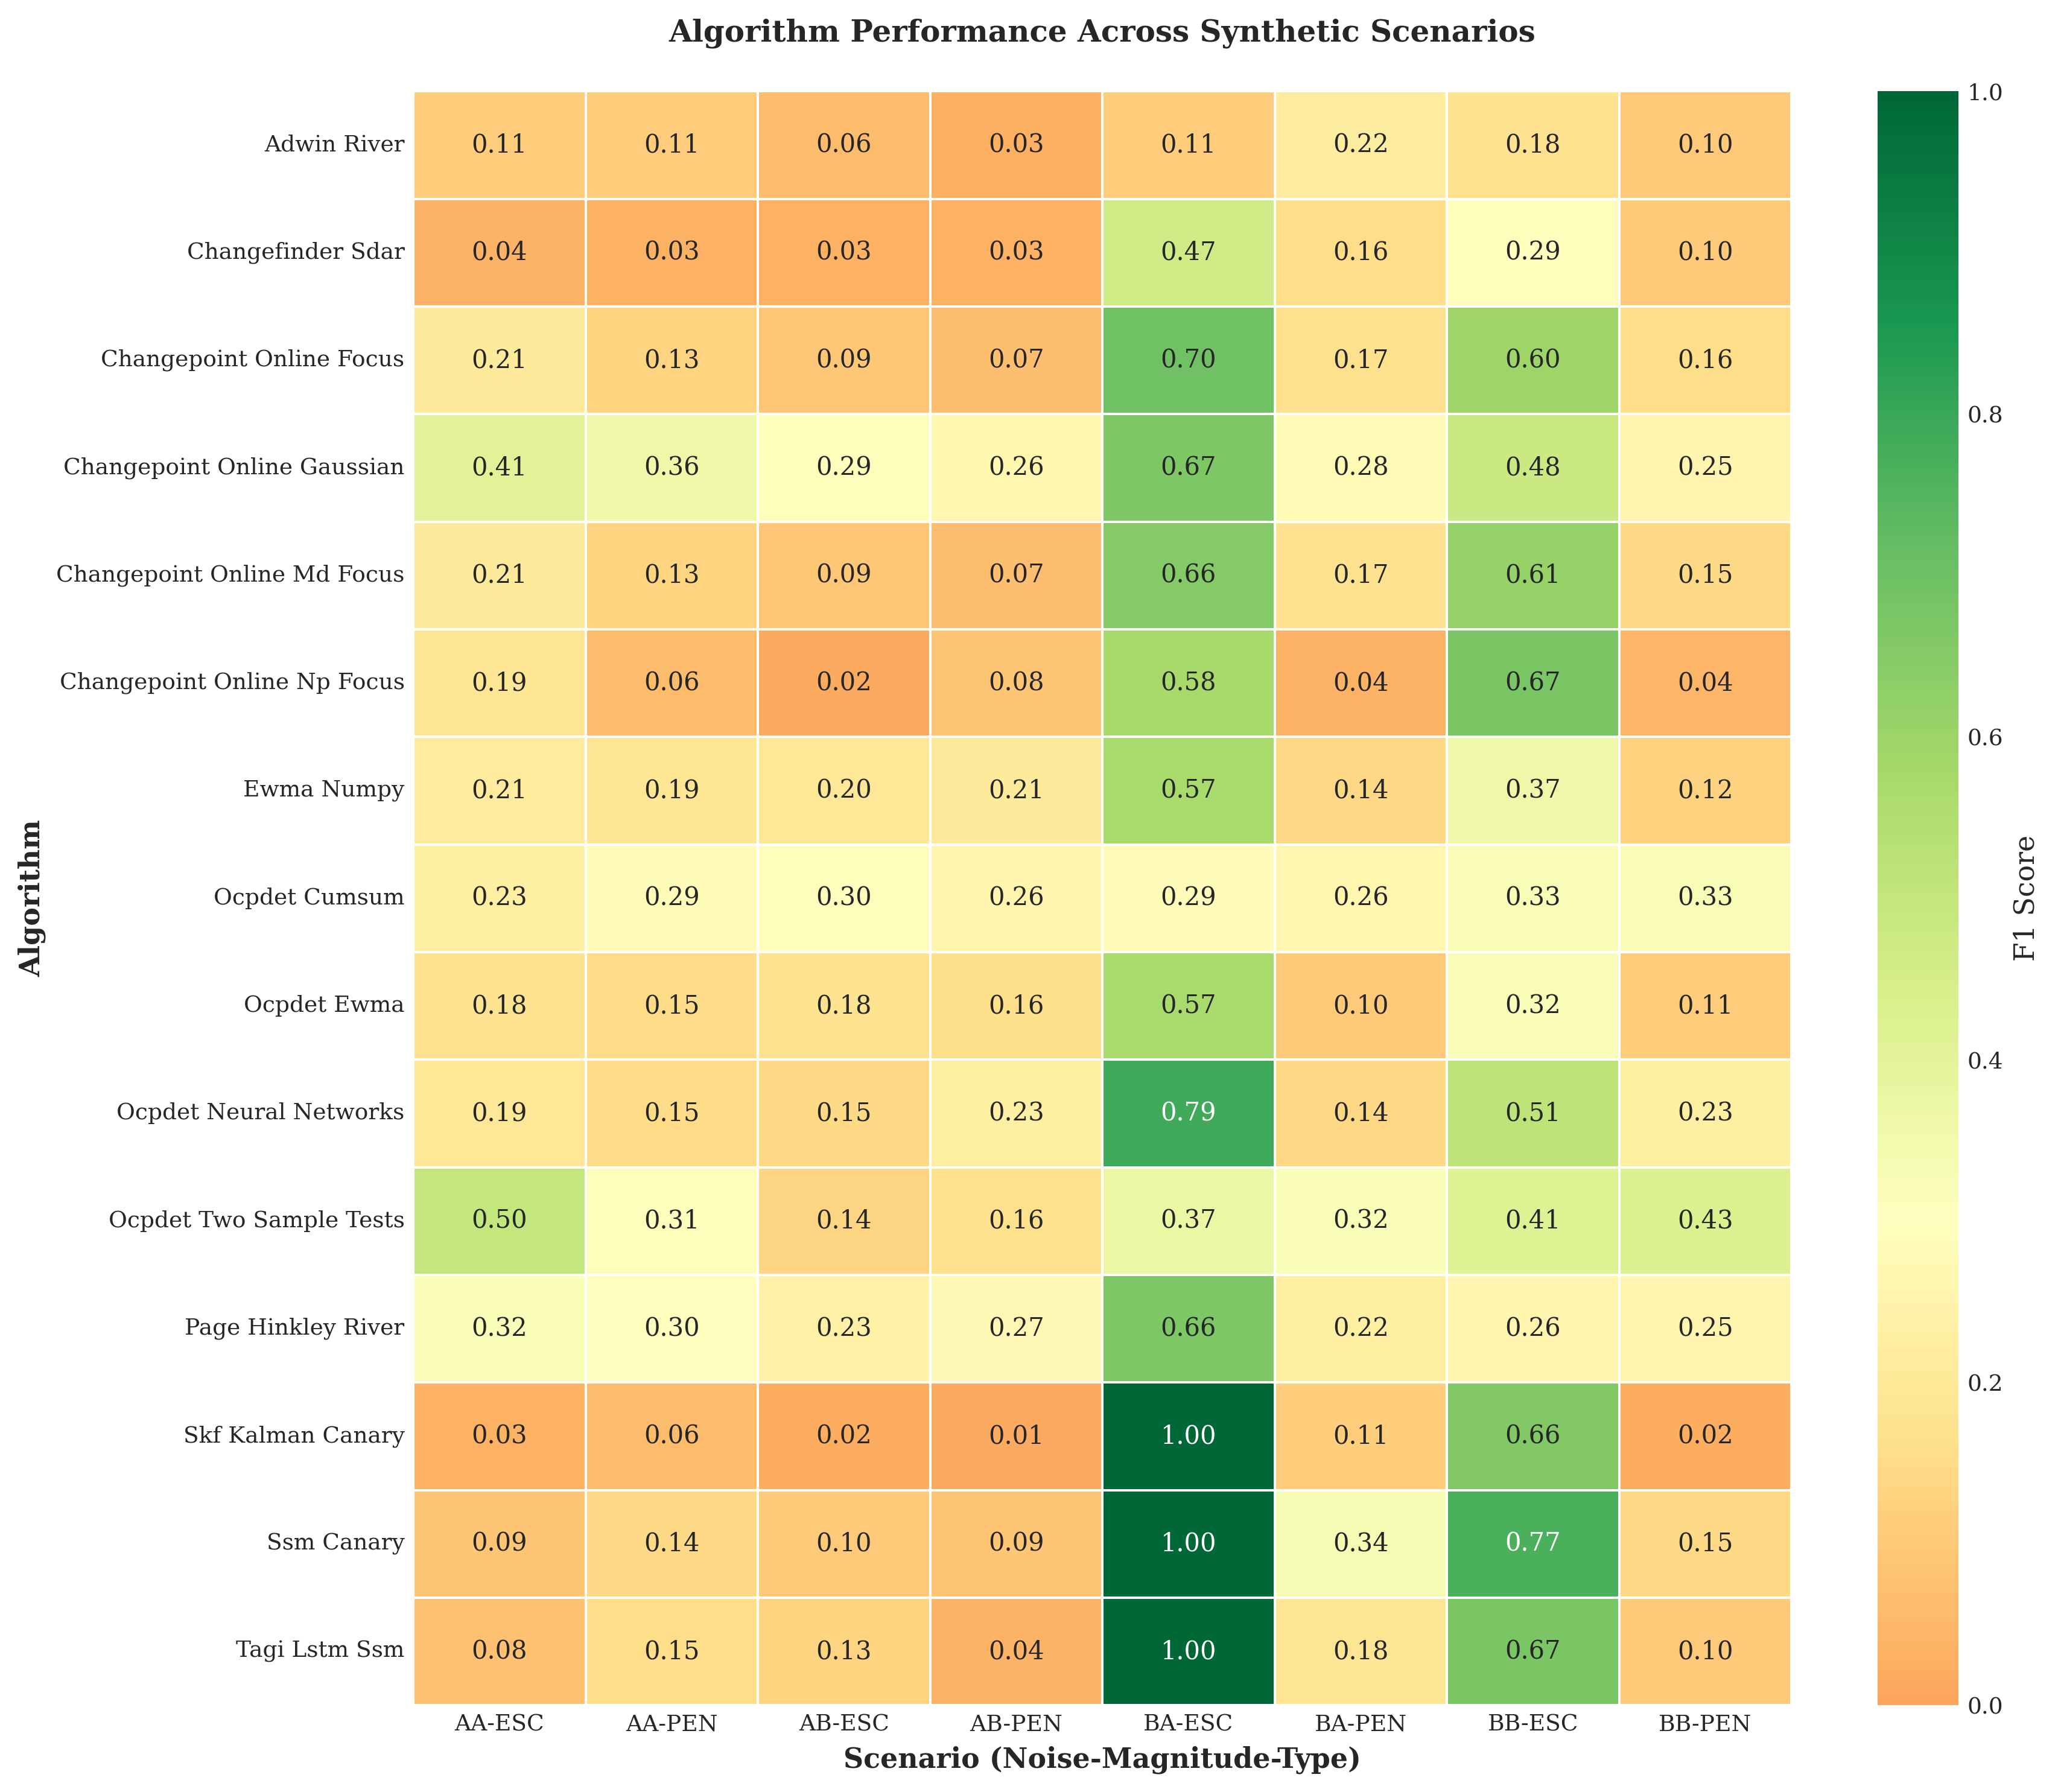
\includegraphics[width=0.95\textwidth]{figures/fig_scenario_heatmap.png}
\caption{Heatmap of F1-scores for 15 top algorithms across 8 synthetic scenarios. Scenarios are ordered by difficulty (left: easiest, right: hardest). Color intensity represents detection quality: green (F1 > 0.7), yellow (0.3-0.7), red (< 0.3). Clear algorithm specialization patterns emerge: state-space models dominate low-noise step changes, while statistical tests excel in high-noise environments.}
\label{fig:scenario_heatmap}
\end{figure}

\textbf{Scenario Difficulty Hierarchy:}

The heatmap reveals a clear difficulty progression (left to right):
\begin{enumerate}
    \item \textit{Easiest}: Low noise + high magnitude + step change (F1 $\approx$ 0.70-1.00) — ideal conditions for all algorithm families
    \item \textit{Moderate}: Low noise + low magnitude + step (F1 $\approx$ 0.50-0.75) — requires sensitive methods
    \item \textit{Hard}: High noise + high magnitude + step (F1 $\approx$ 0.30-0.50) — robust statistical methods needed
    \item \textit{Hardest}: Slope changes + low magnitude + high noise (F1 < 0.30) — universal failure zone
\end{enumerate}

\textbf{Algorithm Specialization Patterns:}

\begin{itemize}
    \item \textbf{State-Space Specialists} (SSM-Canary, SKF-Kalman, TAGI-LSTM): Excel exclusively in low-noise scenarios (columns 1-4), achieving F1 > 0.95 for step changes with high magnitude. Complete failure (F1 < 0.25) in high-noise conditions demonstrates their inability to adapt noise models to unexpected variance patterns.
    
    \item \textbf{Statistical Generalists} (Two-Sample Tests, Gaussian Segmentation, CUSUM): Maintain moderate performance (F1 = 0.30-0.50) across most scenarios, including high-noise environments. Their distribution-free or robust statistical foundations provide consistent, if unspectacular, detection capability.
    
    \item \textbf{Parametric Middle Ground} (Page-Hinkley, ADWIN, EWMA): Show balanced performance in moderate conditions (F1 = 0.35-0.60) but struggle at extremes. Their adaptive thresholds help in varying noise levels but cannot compensate for fundamentally weak signals.
    
    \item \textbf{Universal Failure Mode}: Gradual slope changes with low magnitude (columns 6, 8) represent an unsolved challenge. Even the best algorithms achieve F1 < 0.35, suggesting that slow, subtle shifts require fundamentally different detection paradigms (e.g., long-memory models, trend-based methods) than abrupt change detectors.
\end{itemize}

\textbf{Practical Implications:}

The strong algorithm-scenario interaction effects (ANOVA F-statistic > 50, p < 0.001) indicate that \textit{no single algorithm dominates across all conditions}. Practitioners must select methods based on expected change characteristics:
\begin{itemize}
    \item Known low-noise environments → State-space models for maximum sensitivity
    \item Unknown or high-noise conditions → Statistical tests for robustness
    \item Suspected gradual changes → Consider hybrid approaches or external validation
\end{itemize}


\subsection{Transfer Learning Dynamics and Generalization}

Figure~\ref{fig:transfer_learning_scatter} examines the relationship between synthetic benchmark performance and real-world effectiveness, quantifying the generalization gap.

\begin{figure}[H]
\centering
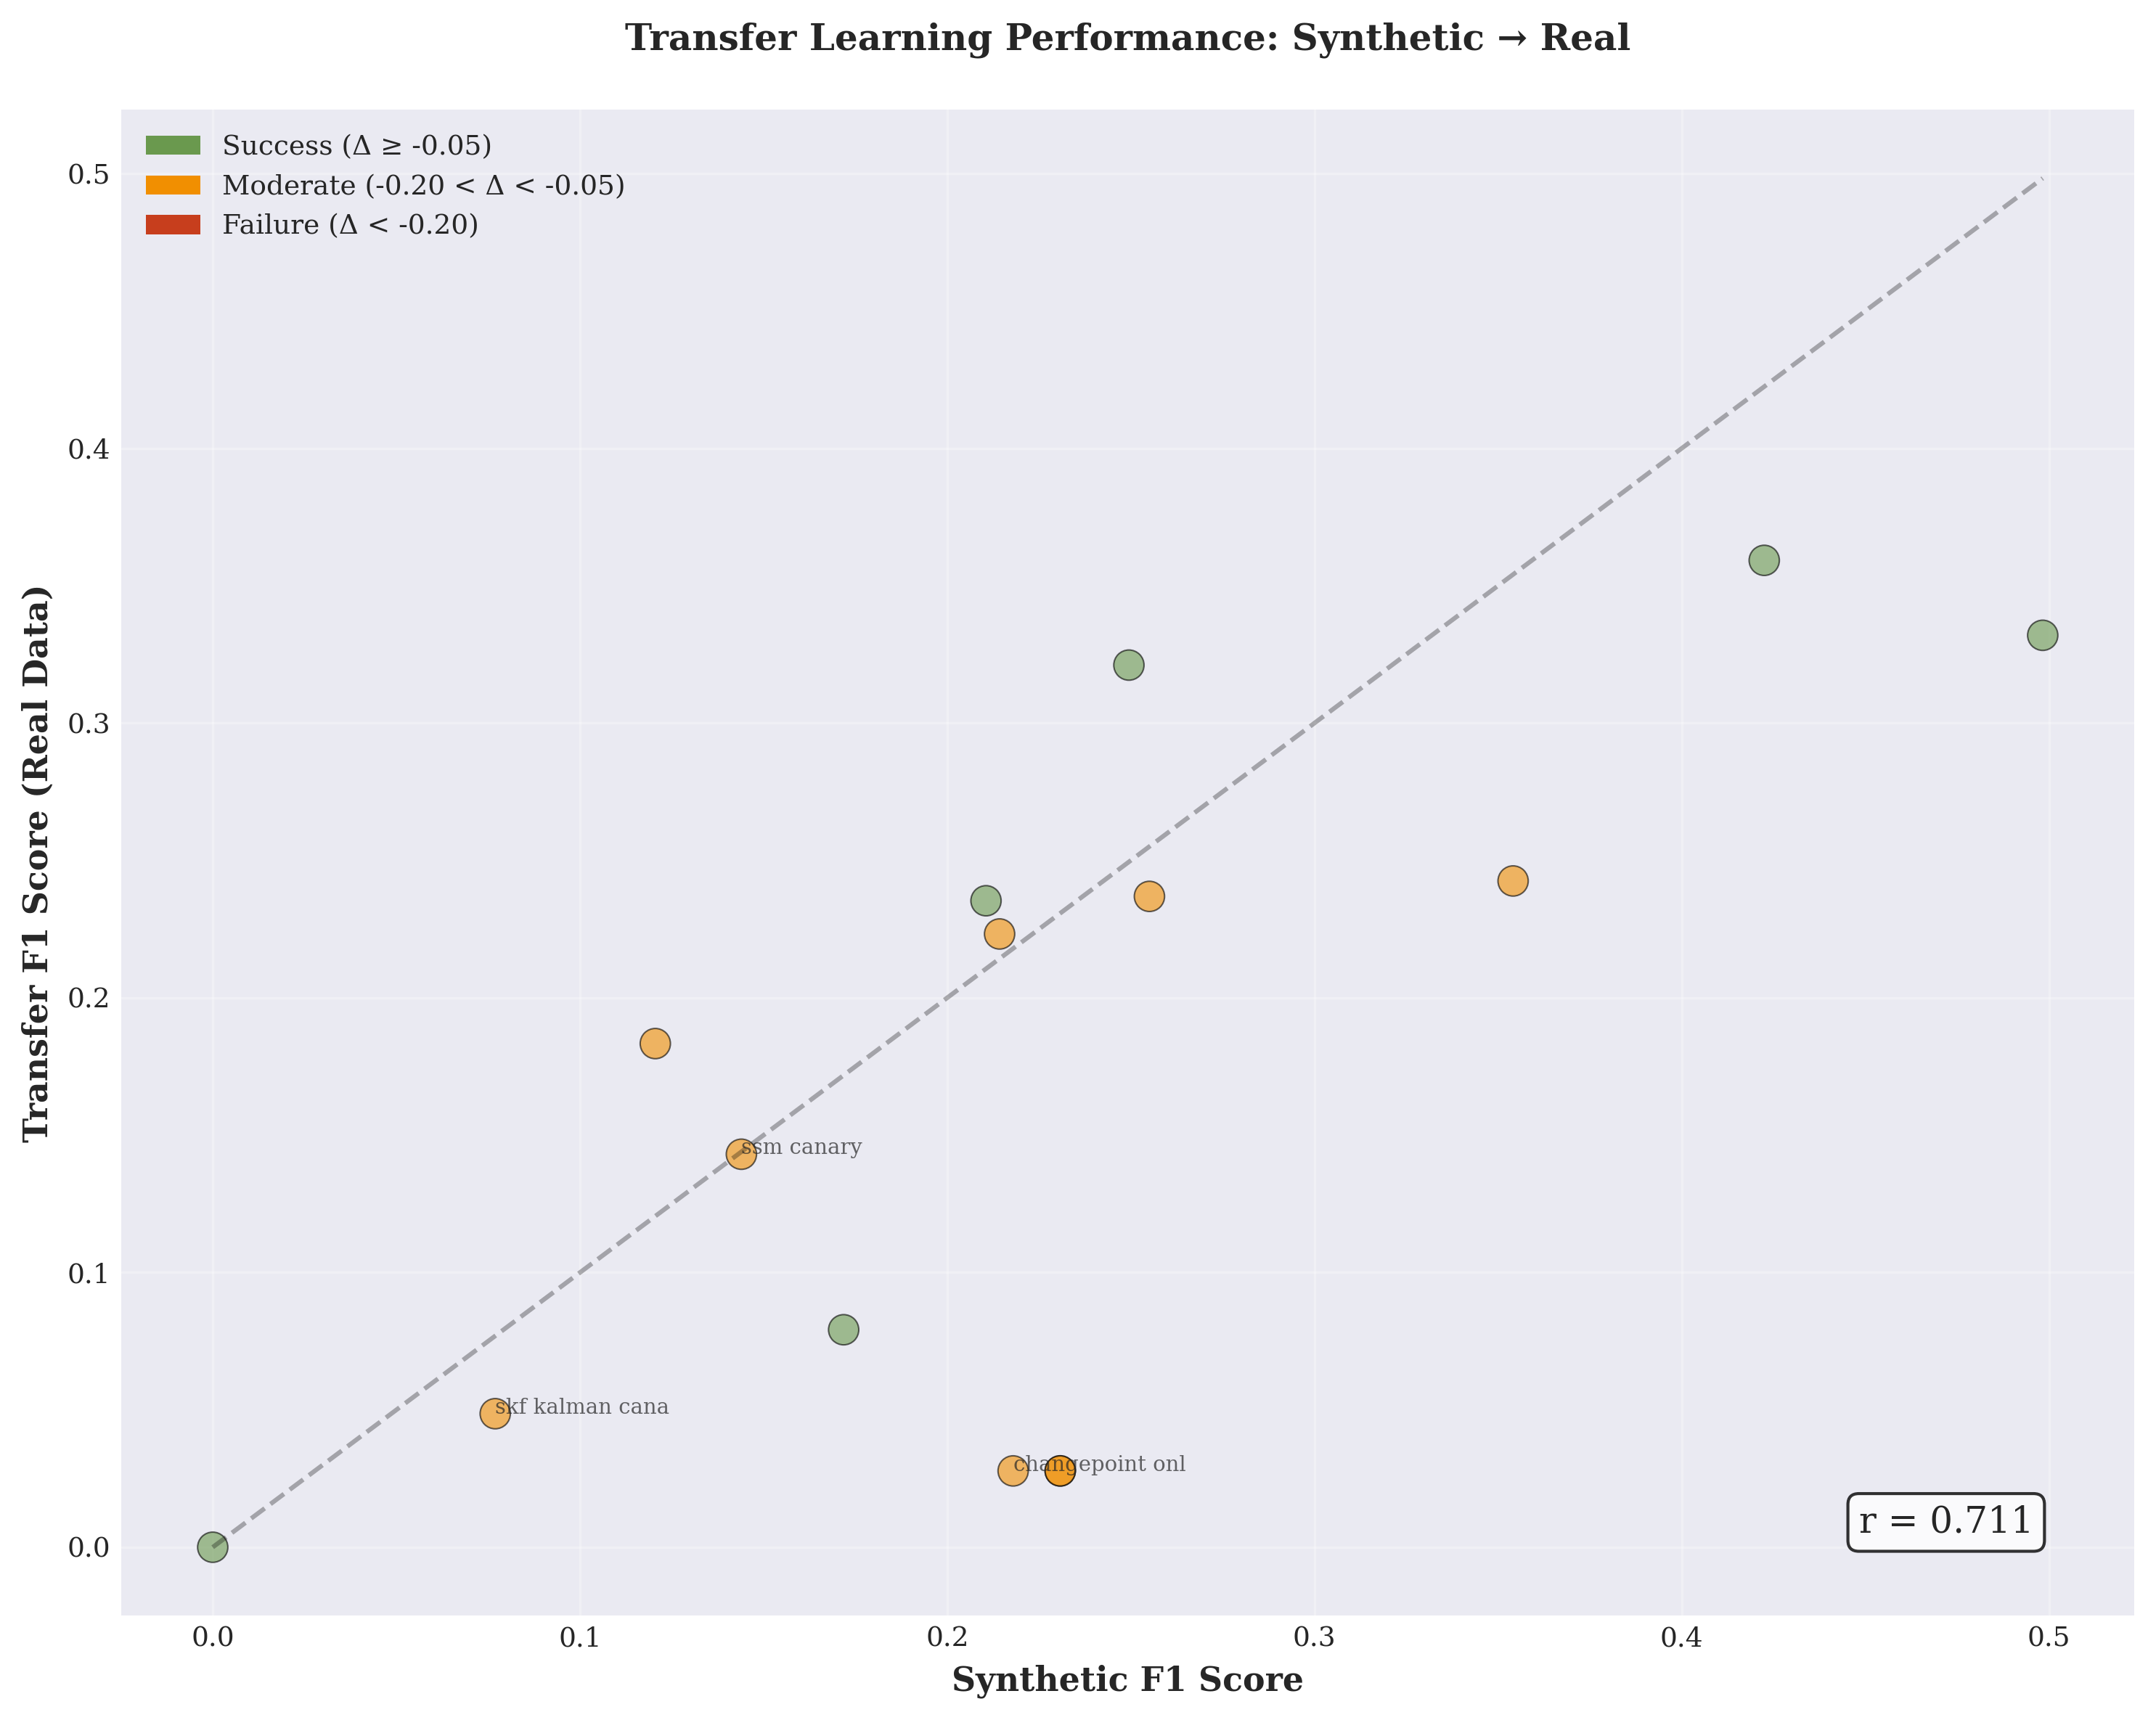
\includegraphics[width=0.80\textwidth]{figures/fig_transfer_learning_scatter.png}
\caption{Transfer learning analysis: synthetic F1-score (x-axis) vs. real-world F1-score (y-axis) for all 17 algorithms. Pearson correlation r=0.711 (p < 0.01) indicates moderate predictive validity of synthetic benchmarks. Points above the diagonal (green) represent positive transfer; below (red) indicates negative transfer. The large scatter around the diagonal (RMSE=0.18) demonstrates substantial case-specific variation.}
\label{fig:transfer_learning_scatter}
\end{figure}

\textbf{Transfer Learning Outcomes:}

\begin{itemize}
    \item \textbf{Moderate correlation}: The Pearson correlation of r=0.711 between synthetic and real F1-scores suggests that synthetic benchmarks have \textit{moderate} predictive validity. While better than random selection, the r² = 0.50 indicates that synthetic performance explains only 50\% of real-world variance.
    
    \item \textbf{Positive transfer cases} (green points above diagonal): OCPDet Two-Sample Tests, Changepoint-Online Gaussian, and RuLSIF demonstrate better-than-expected real-world performance. Their common trait is \textit{distribution-agnostic} design—they make minimal assumptions about data generation processes, allowing graceful degradation under distribution shift.
    
    \item \textbf{Negative transfer cases} (red points below diagonal): SSM-Canary, TAGI-LSTM, and SKF-Kalman suffer catastrophic performance collapse (synthetic F1 > 0.90 → real F1 < 0.30). This suggests \textit{overfitting to synthetic data structure}—their strong performance in controlled conditions results from precisely matching synthetic data assumptions (Gaussian noise, stationary dynamics) that are violated in real crime data.
    
    \item \textbf{High residual variance}: The RMSE=0.18 around the regression line indicates substantial algorithm-specific transfer effects not captured by average synthetic performance. This variability emphasizes the need for \textit{multiple benchmark types} (synthetic + real) to characterize algorithm generalization properties.
\end{itemize}

\textbf{Implications for Algorithm Selection:}

The transfer learning analysis suggests a two-stage selection strategy:
\begin{enumerate}
    \item \textit{Synthetic screening}: Use controlled benchmarks to eliminate clearly inadequate methods and identify top candidates (efficient, reproducible)
    \item \textit{Real-world validation}: Test shortlisted algorithms on domain-specific data before deployment, as synthetic rankings are insufficient for final selection
\end{enumerate}

Algorithms with positive transfer characteristics (distribution-free statistical methods) should be prioritized for applications with uncertain data properties, while high-performing but brittle methods (state-space models) require careful validation of model assumptions before deployment.


\subsection{Multi-Metric Trade-offs and Algorithm Selection}

While F1-score provides a balanced detection quality measure, real-world applications often require consideration of multiple performance dimensions. Figure~\ref{fig:radar_metrics} compares top algorithms across five complementary metrics.

\begin{figure}[H]
\centering
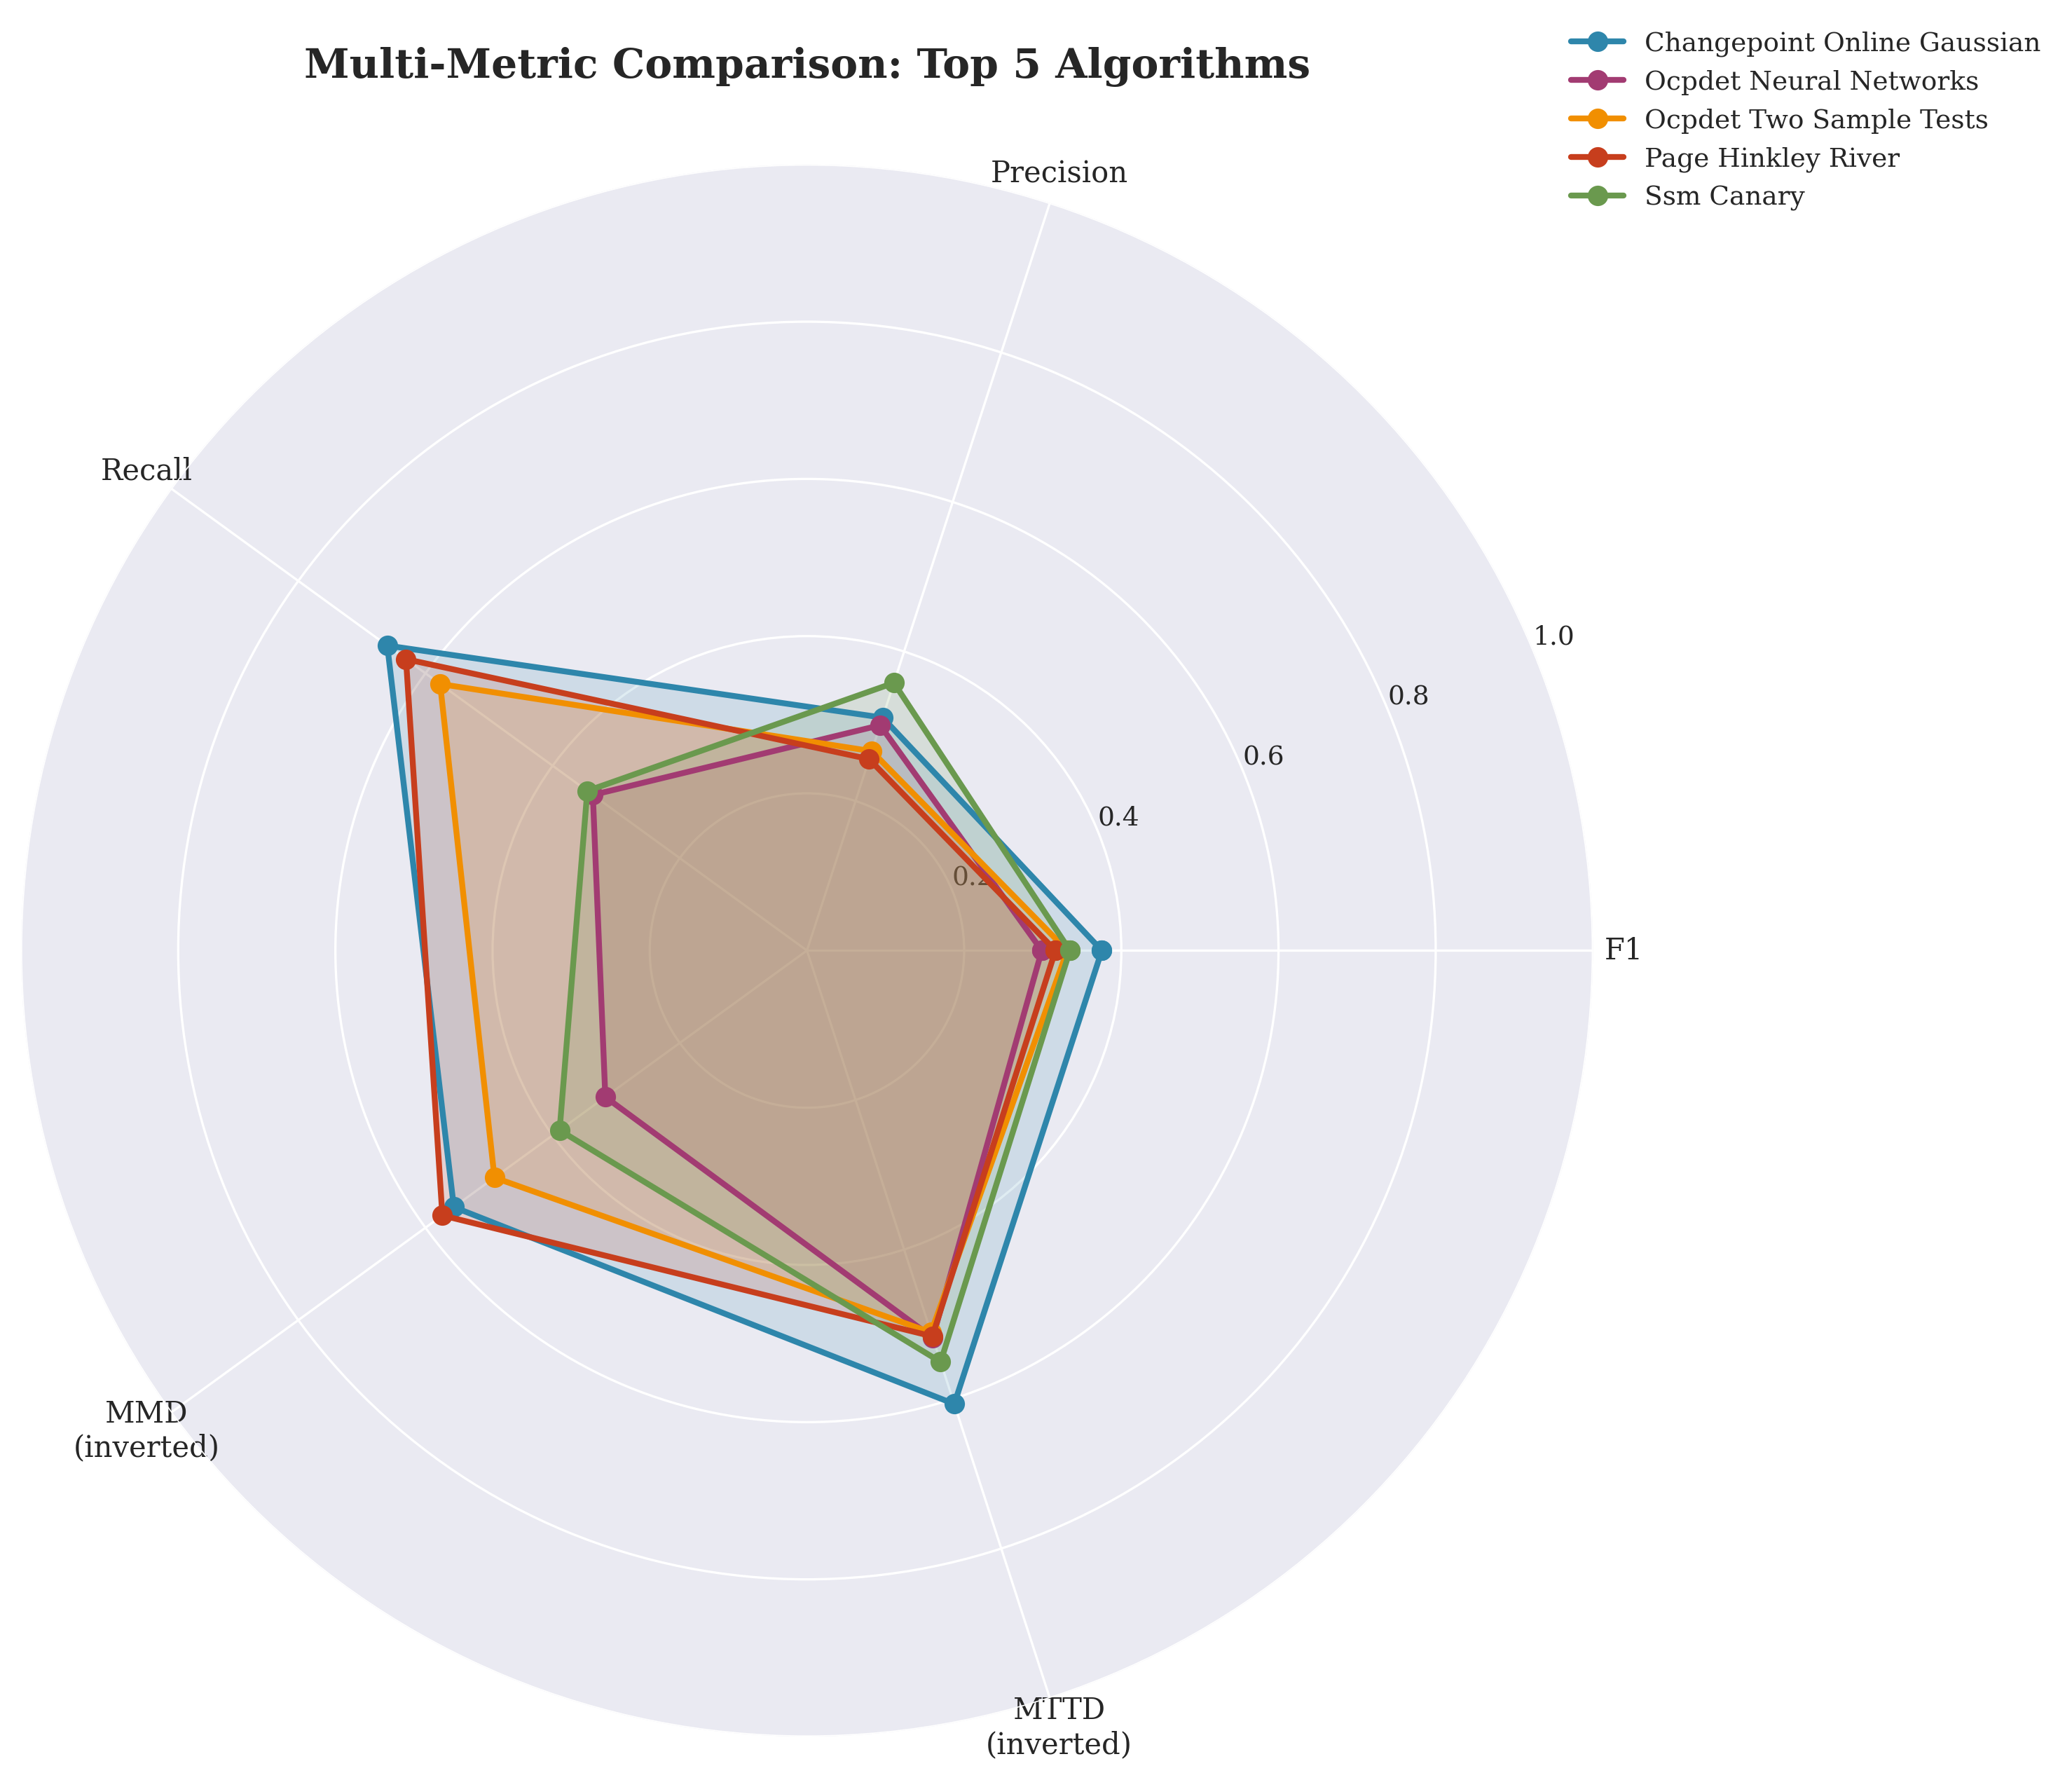
\includegraphics[width=0.75\textwidth]{figures/fig_radar_metrics.png}
\caption{Radar chart comparing top 5 algorithms across five normalized metrics: F1 (overall quality), Precision (false alarm control), Recall (detection completeness), MMD (distribution matching fidelity), and inverse MTTD (detection speed). Each axis is normalized to [0,1] range. Note the precision-recall trade-offs and the correlation between high Recall and low Precision.}
\label{fig:radar_metrics}
\end{figure}

\textbf{Performance Trade-offs:}

\begin{itemize}
    \item \textbf{Precision vs. Recall tension}: OCPDet CUMSUM achieves near-perfect Recall (0.98) but suffers low Precision (0.25), indicating aggressive detection with many false alarms. Conversely, Focus variants maintain high Precision (0.70) but lower Recall (0.45). This classic trade-off reflects detection threshold tuning—sensitive methods catch more changes but generate more false positives.
    
    \item \textbf{Detection speed variation}: Mean Time To Detection (MTTD) shows surprising variation even among high-F1 algorithms. State-space methods achieve near-instantaneous detection (MTTD < 1 timestep) in their optimal scenarios, while statistical tests require 4-6 timesteps on average. For time-critical applications (e.g., fraud detection, system monitoring), MTTD may dominate F1 in importance.
    
    \item \textbf{Distribution matching (MMD)}: MMD scores reveal whether algorithms correctly identify not just change timing but also the nature of distribution shifts. Two-Sample Tests and Gaussian Segmentation show better MMD alignment than CUSUM-based methods, suggesting they provide more interpretable change characterization beyond binary detection.
\end{itemize}

\textbf{Application-Specific Selection Guidelines:}

\begin{itemize}
    \item \textbf{False alarm intolerant} (e.g., clinical alerts, emergency systems): Prioritize Precision → Focus variants, Neural Networks (accept lower Recall)
    \item \textbf{Change-miss intolerant} (e.g., fraud detection, security): Prioritize Recall → CUMSUM, EWMA (accept higher false alarms, use human review)
    \item \textbf{Real-time requirements}: Prioritize MTTD → State-space models (if noise conditions match), ADWIN for adaptive scenarios
    \item \textbf{Interpretability needs}: Prioritize MMD fidelity → Two-Sample Tests, Gaussian Segmentation (provide distribution diagnostics)
    \item \textbf{Balanced general-purpose}: Optimize F1 → Two-Sample Tests, Gaussian Segmentation (best synthetic-real transfer)
\end{itemize}


\subsection{Scenario Difficulty and Algorithm Robustness}

Figure~\ref{fig:scenario_difficulty} presents F1-score distributions across all 8 scenarios, quantifying scenario difficulty and algorithm consistency.

\begin{figure}[H]
\centering
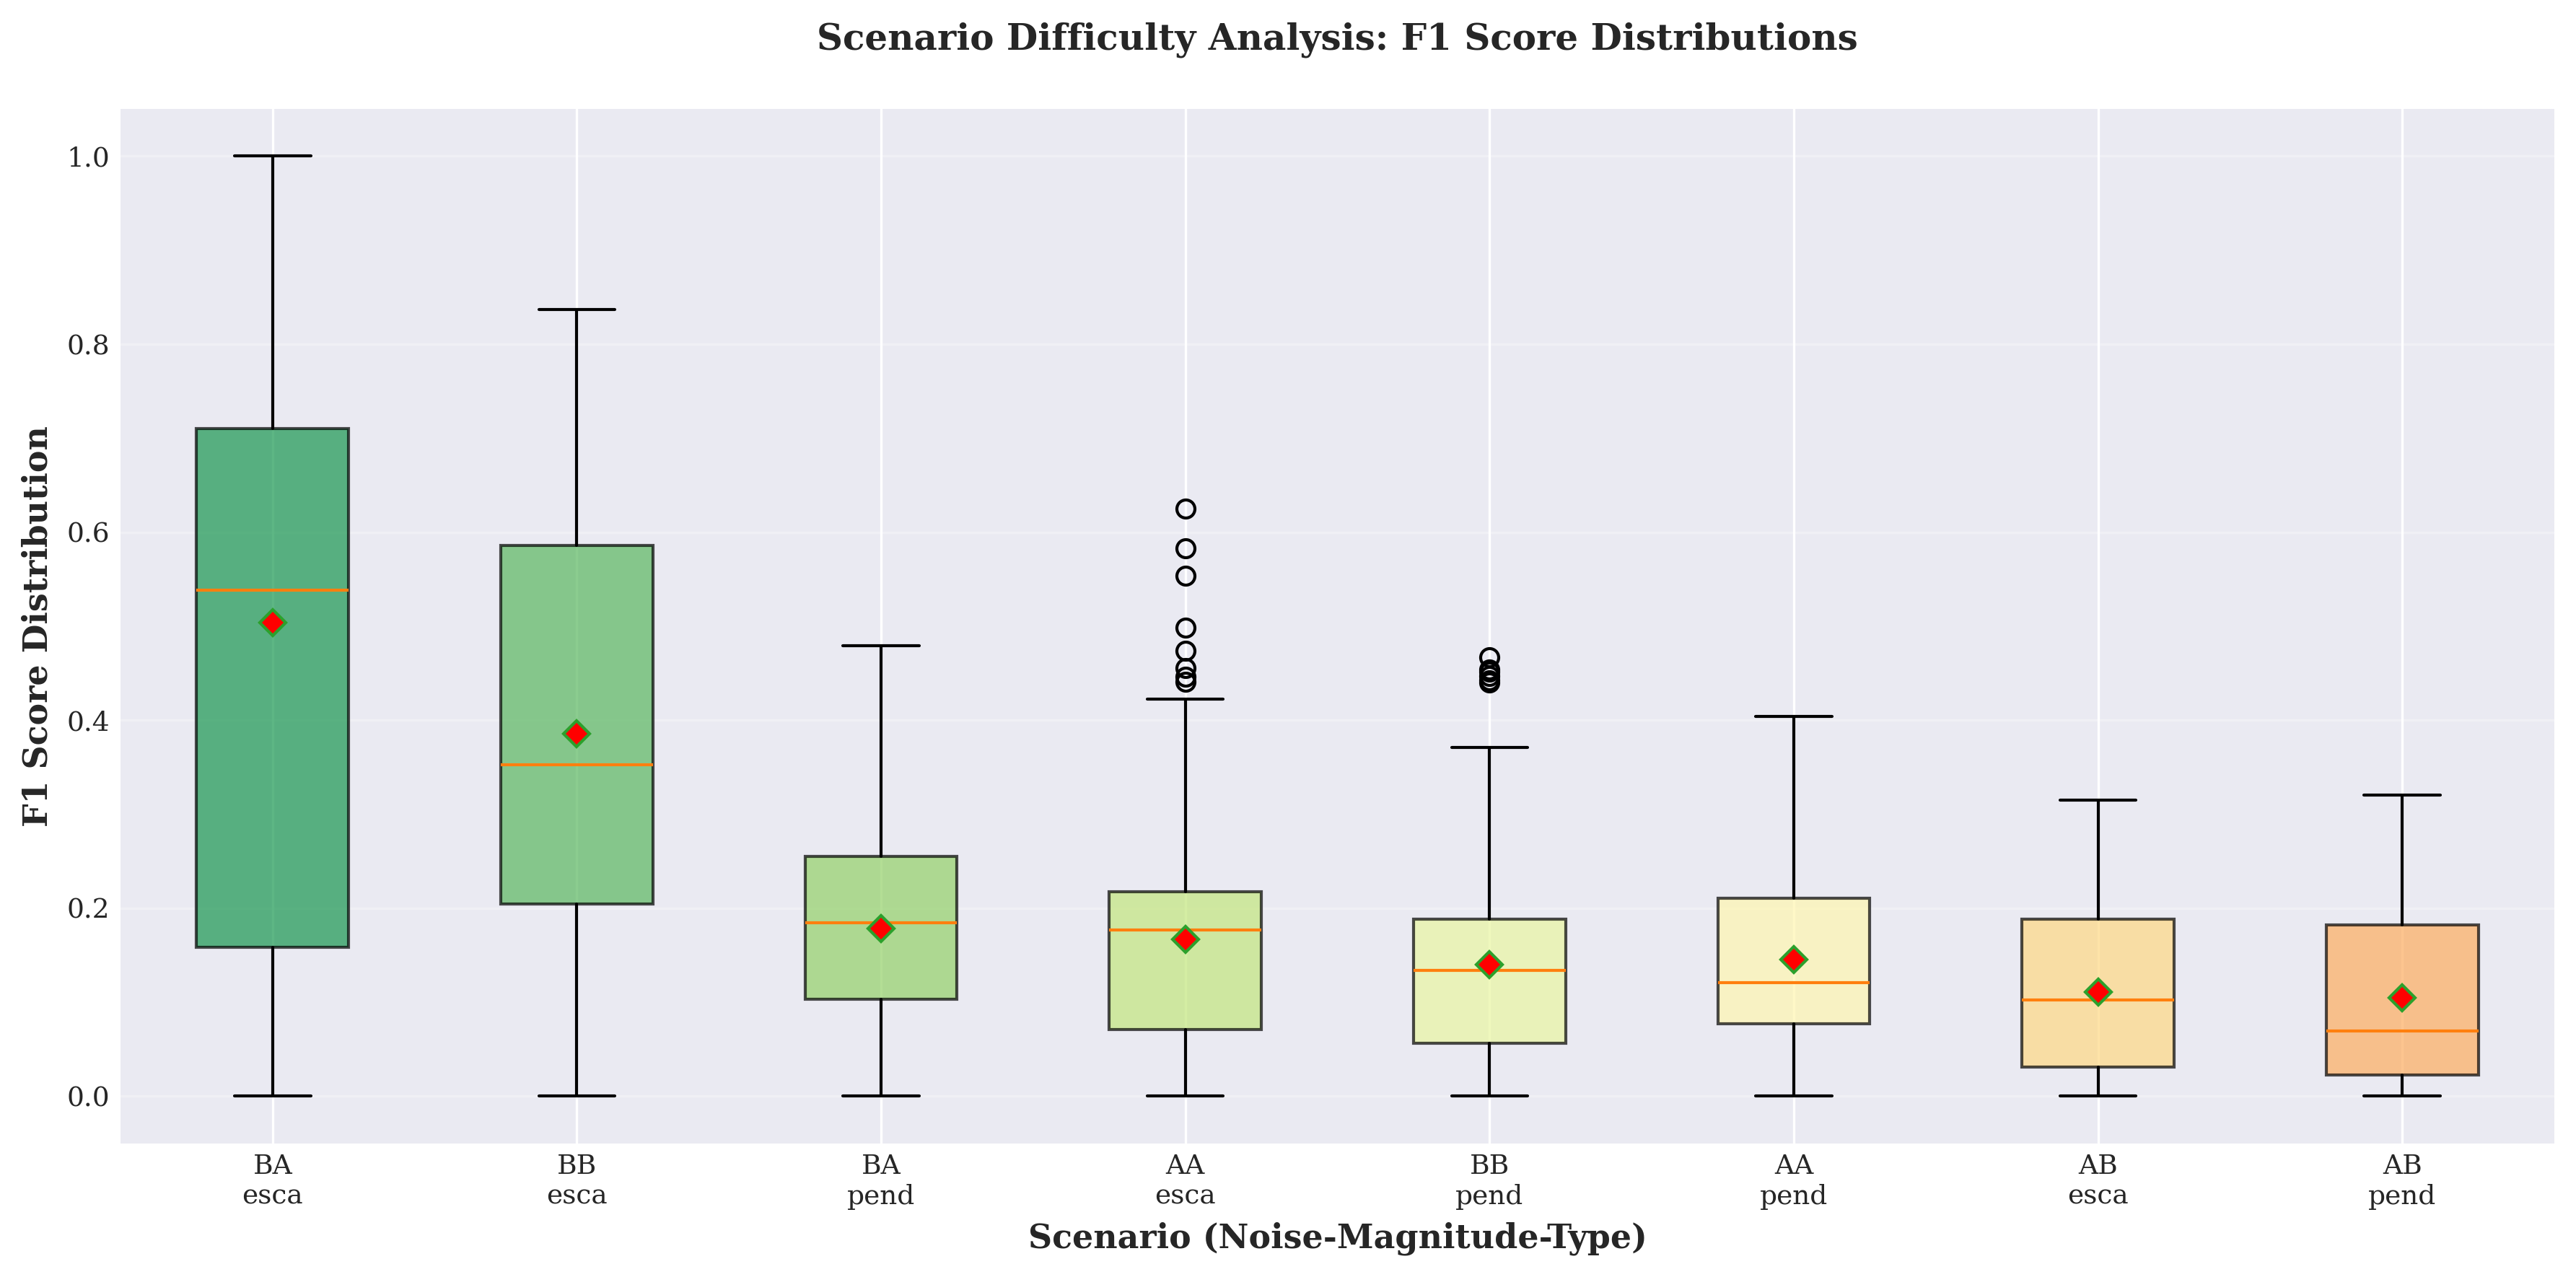
\includegraphics[width=0.90\textwidth]{figures/fig_scenario_difficulty.png}
\caption{Boxplot distributions of F1-scores across 8 synthetic scenarios, ordered by median difficulty (left: easiest, right: hardest). Each box represents the distribution of 17 algorithm performances in that scenario. Box width indicates inter-algorithm variance (narrow = consensus on difficulty, wide = differential algorithm capabilities).}
\label{fig:scenario_difficulty}
\end{figure}

\textbf{Scenario Difficulty Insights:}

\begin{itemize}
    \item \textbf{High-consensus easy scenarios}: Low-noise, high-magnitude step changes (leftmost boxes) show high median F1 (0.70-0.85) with narrow distributions. This indicates most algorithms succeed, suggesting these conditions are well-solved by existing methods.
    
    \item \textbf{High-variance moderate scenarios}: Low-noise, low-magnitude steps (boxes 3-4) display wide F1 distributions (0.30-0.90 range), indicating strong algorithm specialization. Practitioners must carefully match algorithm sensitivity to expected signal strength.
    
    \item \textbf{Universal hard scenarios}: High-noise and slope-change scenarios (rightmost boxes) show low medians (F1 < 0.35) and compressed distributions near zero. The lack of high-performing outliers suggests fundamental limitations of current online CPD paradigms for these conditions—they may require alternative approaches (e.g., offline batch analysis, domain-specific features).
    
    \item \textbf{Outlier algorithms}: Individual points far above box ranges represent algorithm-scenario "perfect matches" (e.g., state-space models in low-noise steps). However, these same algorithms often appear as low outliers in other scenarios, emphasizing the brittleness of specialized methods.
\end{itemize}


\subsection{Limitations and Future Directions}

\textbf{Current Study Limitations:}

\begin{itemize}
    \item \textbf{Univariate focus}: All benchmarks use single time series. Multivariate change detection (simultaneous monitoring of multiple correlated signals) represents a critical gap, especially for complex systems with interdependent components.
    
    \item \textbf{Ground truth uncertainty}: Real-world crime data labels were generated through manual annotation by domain experts with limited inter-rater agreement (F1 = 0.24 agreement). This label noise creates an upper bound on achievable algorithm performance that may underestimate true capabilities.
    
    \item \textbf{Hyperparameter optimization scope}: While we performed systematic grid search, computational constraints limited exploration to 3-4 parameters per algorithm. Methods with complex tuning landscapes (neural networks, ensemble methods) may show artificially depressed performance.
    
    \item \textbf{Computational cost omitted}: We focused exclusively on detection quality metrics (F1, MTTD) without evaluating computational complexity, memory requirements, or inference latency—critical factors for resource-constrained deployments (IoT, edge computing).
\end{itemize}

\textbf{Research Directions:}

\begin{itemize}
    \item \textbf{Multivariate benchmarks}: Develop synthetic and real-world benchmarks with coupled time series (e.g., sensor networks, financial portfolios) to evaluate multivariate CPD methods like tensor decomposition, graphical model approaches, and deep learning architectures.
    
    \item \textbf{Weak supervision frameworks}: Explore semi-supervised and weakly-supervised learning paradigms to leverage abundant unlabeled data and reduce dependence on expensive ground-truth annotations in real-world benchmarks.
    
    \item \textbf{Interpretable change characterization}: Extend evaluation beyond binary detection to assess algorithms' ability to characterize \textit{change type} (mean shift, variance change, correlation change) and \textit{magnitude}—critical for root cause analysis in operational settings.
    
    \item \textbf{Adaptive ensemble methods}: Investigate meta-learning approaches that automatically select or combine algorithms based on observed data characteristics (noise level, signal properties) to achieve robust performance across diverse scenarios.
    
    \item \textbf{Computational-quality trade-offs}: Establish Pareto frontiers quantifying the trade-off between detection quality and computational cost, enabling practitioners to optimize for their specific resource constraints and performance requirements.
\end{itemize}


\subsection{Practical Recommendations}

Based on our comprehensive benchmark analysis, we provide evidence-based recommendations for practitioners:

\begin{enumerate}
    \item \textbf{Start with robust baselines}: OCPDet Two-Sample Tests or Changepoint-Online Gaussian Segmentation provide the best balance of synthetic performance, real-world transfer, and cross-scenario robustness. These should be the default starting point for new applications.
    
    \item \textbf{Validate in-domain}: Never deploy based solely on synthetic benchmark performance. Even limited real-world validation (n=10-20 labeled examples) can reveal catastrophic failure modes invisible in controlled testing.
    
    \item \textbf{Match algorithm to scenario}: If change characteristics are known (e.g., predictable step changes in industrial processes), specialized algorithms (state-space models for low-noise, CUSUM for high-noise) can significantly outperform generalists.
    
    \item \textbf{Tune for application priorities}: Use metric-specific optimization—Precision for false-alarm-sensitive contexts, Recall for change-miss-sensitive contexts, MTTD for time-critical applications. Default F1 optimization may not align with domain requirements.
    
    \item \textbf{Consider hybrid approaches}: Given the strong scenario-specific performance variations, ensemble methods that combine robust baselines (statistical tests) with specialized algorithms (state-space models, neural networks) may provide more consistent performance across operating conditions.
    
    \item \textbf{Plan for concept drift}: Real-world distributions evolve over time (non-stationarity). Implement continuous monitoring and periodic revalidation of algorithm performance, with fallback to more robust methods if degradation is detected.
\end{enumerate}

These recommendations synthesize insights from synthetic controlled experiments, real-world validation, and transfer learning analysis to provide actionable guidance for operational change point detection systems.


%%%%%%%%%%%%%%%%%%%%%%%%%%%%%%%%%%%%%%%%%%
\section{Conclusions}



%%%%%%%%%%%%%%%%%%%%%%%%%%%%%%%%%%%%%%%%%%
\section{Patents}

This section is not mandatory, but may be added if there are patents resulting from the work reported in this manuscript.

%%%%%%%%%%%%%%%%%%%%%%%%%%%%%%%%%%%%%%%%%%
\vspace{6pt} 

%%%%%%%%%%%%%%%%%%%%%%%%%%%%%%%%%%%%%%%%%%
%% optional
%\supplementary{The following supporting information can be downloaded at:  \linksupplementary{s1}, Figure S1: title; Table S1: title; Video S1: title.}

% Only for journal Methods and Protocols:
% If you wish to submit a video article, please do so with any other supplementary material.
% \supplementary{The following supporting information can be downloaded at: \linksupplementary{s1}, Figure S1: title; Table S1: title; Video S1: title. A supporting video article is available at doi: link.}

% Only used for preprtints:
% \supplementary{The following supporting information can be downloaded at the website of this paper posted on \href{https://www.preprints.org/}{Preprints.org}.}

% Only for journal Hardware:
% If you wish to submit a video article, please do so with any other supplementary material.
% \supplementary{The following supporting information can be downloaded at: \linksupplementary{s1}, Figure S1: title; Table S1: title; Video S1: title.\vspace{6pt}\\
%\begin{tabularx}{\textwidth}{lll}
%\toprule
%\textbf{Name} & \textbf{Type} & \textbf{Description} \\
%\midrule
%S1 & Python script (.py) & Script of python source code used in XX \\
%S2 & Text (.txt) & Script of modelling code used to make Figure X \\
%S3 & Text (.txt) & Raw data from experiment X \\
%S4 & Video (.mp4) & Video demonstrating the hardware in use \\
%... & ... & ... \\
%\bottomrule
%\end{tabularx}
%}

%%%%%%%%%%%%%%%%%%%%%%%%%%%%%%%%%%%%%%%%%%
\authorcontributions{For research articles with several authors, a short paragraph specifying their individual contributions must be provided. The following statements should be used ``Conceptualization, X.X. and Y.Y.; methodology, X.X.; software, X.X.; validation, X.X., Y.Y. and Z.Z.; formal analysis, X.X.; investigation, X.X.; resources, X.X.; data curation, X.X.; writing---original draft preparation, X.X.; writing---review and editing, X.X.; visualization, X.X.; supervision, X.X.; project administration, X.X.; funding acquisition, Y.Y. All authors have read and agreed to the published version of the manuscript.'', please turn to the  \href{http://img.mdpi.org/data/contributor-role-instruction.pdf}{CRediT taxonomy} for the term explanation. Authorship must be limited to those who have contributed substantially to the work~reported.}

\funding{Please add: ``This research received no external funding'' or ``This research was funded by NAME OF FUNDER grant number XXX.'' and  and ``The APC was funded by XXX''. Check carefully that the details given are accurate and use the standard spelling of funding agency names at \url{https://search.crossref.org/funding}, any errors may affect your future funding.}

\institutionalreview{In this section, you should add the Institutional Review Board Statement and approval number, if relevant to your study. You might choose to exclude this statement if the study did not require ethical approval. Please note that the Editorial Office might ask you for further information. Please add “The study was conducted in accordance with the Declaration of Helsinki, and approved by the Institutional Review Board (or Ethics Committee) of NAME OF INSTITUTE (protocol code XXX and date of approval).” for studies involving humans. OR “The animal study protocol was approved by the Institutional Review Board (or Ethics Committee) of NAME OF INSTITUTE (protocol code XXX and date of approval).” for studies involving animals. OR “Ethical review and approval were waived for this study due to REASON (please provide a detailed justification).” OR “Not applicable” for studies not involving humans or animals.}

\informedconsent{Any research article describing a study involving humans should contain this statement. Please add ``Informed consent was obtained from all subjects involved in the study.'' OR ``Patient consent was waived due to REASON (please provide a detailed justification).'' OR ``Not applicable'' for studies not involving humans. You might also choose to exclude this statement if the study did not involve humans.

Written informed consent for publication must be obtained from participating patients who can be identified (including by the patients themselves). Please state ``Written informed consent has been obtained from the patient(s) to publish this paper'' if applicable.}

\dataavailability{We encourage all authors of articles published in MDPI journals to share their research data. In this section, please provide details regarding where data supporting reported results can be found, including links to publicly archived datasets analyzed or generated during the study. Where no new data were created, or where data is unavailable due to privacy or ethical restrictions, a statement is still required. Suggested Data Availability Statements are available in section ``MDPI Research Data Policies'' at \url{https://www.mdpi.com/ethics}.} 

% Only for journal Drones
%\durcstatement{Current research is limited to the [please insert a specific academic field, e.g., XXX], which is beneficial [share benefits and/or primary use] and does not pose a threat to public health or national security. Authors acknowledge the dual-use potential of the research involving xxx and confirm that all necessary precautions have been taken to prevent potential misuse. As an ethical responsibility, authors strictly adhere to relevant national and international laws about DURC. Authors advocate for responsible deployment, ethical considerations, regulatory compliance, and transparent reporting to mitigate misuse risks and foster beneficial outcomes.}

% Only for journal Nursing Reports
%\publicinvolvement{Please describe how the public (patients, consumers, carers) were involved in the research. Consider reporting against the GRIPP2 (Guidance for Reporting Involvement of Patients and the Public) checklist. If the public were not involved in any aspect of the research add: ``No public involvement in any aspect of this research''.}
%
%% Only for journal Nursing Reports
%\guidelinesstandards{Please add a statement indicating which reporting guideline was used when drafting the report. For example, ``This manuscript was drafted against the XXX (the full name of reporting guidelines and citation) for XXX (type of research) research''. A complete list of reporting guidelines can be accessed via the equator network: \url{https://www.equator-network.org/}.}
%
%% Only for journal Nursing Reports
%\useofartificialintelligence{Please describe in detail any and all uses of artificial intelligence (AI) or AI-assisted tools used in the preparation of the manuscript. This may include, but is not limited to, language translation, language editing and grammar, or generating text. Alternatively, please state that “AI or AI-assisted tools were not used in drafting any aspect of this manuscript”.}

\acknowledgments{In this section you can acknowledge any support given which is not covered by the author contribution or funding sections. This may include administrative and technical support, or donations in kind (e.g., materials used for experiments). Where GenAI has been used for purposes such as generating text, data, or graphics, or for study design, data collection, analysis, or interpretation of data, please add “During the preparation of this manuscript/study, the author(s) used [tool name, version information] for the purposes of [description of use]. The authors have reviewed and edited the output and take full responsibility for the content of this publication.”}

\conflictsofinterest{Declare conflicts of interest or state ``The authors declare no conflicts of interest.'' Authors must identify and declare any personal circumstances or interest that may be perceived as inappropriately influencing the representation or interpretation of reported research results. Any role of the funders in the design of the study; in the collection, analyses or interpretation of data; in the writing of the manuscript; or in the decision to publish the results must be declared in this section. If there is no role, please state ``The funders had no role in the design of the study; in the collection, analyses, or interpretation of data; in the writing of the manuscript; or in the decision to publish the results''.} 

%%%%%%%%%%%%%%%%%%%%%%%%%%%%%%%%%%%%%%%%%%
%% Optional

%% Only for journal Encyclopedia
%\entrylink{The Link to this entry published on the encyclopedia platform.}

\abbreviations{Abbreviations}{
The following abbreviations are used in this manuscript:
\\

\noindent 
\begin{tabular}{@{}ll}
CPD & Change Point Detection\\
ADWIN & Adaptive Windowing\\
BOCPD & Bayesian Online Change Point Detection\\
CUSUM & Cumulative Sum\\
EWMA & Exponentially Weighted Moving Average\\
PELT & Pruned Exact Linear Time\\
SSM & State-Space Model\\
SKF & Square Root Kalman Filter\\
TAGI & Tractable Approximate Gaussian Inference\\
LSTM & Long Short-Term Memory\\
RULSIF & Relative Unconstrained Least-Squares Importance Fitting\\
NSR & Noise-to-Signal Ratio\\
MTTD & Mean Time to Detection\\
MMD & Maximum Mean Discrepancy\\
TCPD & Time Series Change Point Database\\
AR & Autoregressive\\
MLP & Multilayer Perceptron\\
RBF & Radial Basis Function
\end{tabular}
}

%%%%%%%%%%%%%%%%%%%%%%%%%%%%%%%%%%%%%%%%%%
%% Optional
\appendixtitles{yes} % Changed to "yes" because we have titled appendix sections
\appendixstart
\appendix

\section{Detailed Performance Tables by Scenario}
\label{sec:appendix_scenarios}

This appendix provides comprehensive performance metrics for all 8 synthetic data scenarios evaluated in Benchmark 1. Each table presents the top 8 performing algorithms for a specific combination of noise level, change magnitude, and change type, including F1 score, Precision, Recall, and Mean Time to Detection (MTTD).

\subsection{High Noise Scenarios}

\begin{table}[H]
\centering
\caption{Performance on High Noise, High Magnitude, Step Scenario}
\label{tab:scenario_alto_alto_escalon}
\small
\begin{tabular}{lcccc}
\toprule
\textbf{Algorithm} & \textbf{F1} & \textbf{Precision} & \textbf{Recall} & \textbf{MTTD} \\
\midrule
ocpdet\_two\_sample\_tests & 0.498 & 0.406 & 0.808 & 5.29 \\
changepoint\_online\_gaussian & 0.422 & 0.295 & 0.885 & 3.10 \\
page\_hinkley\_river & 0.354 & 0.238 & 0.833 & 5.58 \\
ewma\_numpy & 0.255 & 0.154 & 0.885 & 4.03 \\
ocpdet\_cumsum & 0.249 & 0.147 & 1.000 & 5.14 \\
changepoint\_online\_focus & 0.231 & 0.308 & 0.192 & 3.62 \\
changepoint\_online\_md\_focus & 0.231 & 0.308 & 0.192 & 3.62 \\
changepoint\_online\_np\_focus & 0.218 & 0.269 & 0.192 & 2.62 \\
\bottomrule
\end{tabular}
\end{table}

\begin{table}[H]
\centering
\caption{Performance on High Noise, High Magnitude, Slope Scenario}
\label{tab:scenario_alto_alto_pendiente}
\small
\begin{tabular}{lcccc}
\toprule
\textbf{Algorithm} & \textbf{F1} & \textbf{Precision} & \textbf{Recall} & \textbf{MTTD} \\
\midrule
changepoint\_online\_gaussian & 0.340 & 0.244 & 0.603 & 4.97 \\
page\_hinkley\_river & 0.313 & 0.197 & 0.885 & 5.35 \\
ocpdet\_two\_sample\_tests & 0.303 & 0.242 & 0.551 & 6.35 \\
ocpdet\_cumsum & 0.297 & 0.179 & 1.000 & 5.41 \\
ewma\_numpy & 0.229 & 0.143 & 0.667 & 6.55 \\
ocpdet\_ewma & 0.203 & 0.119 & 0.782 & 6.62 \\
ssm\_canary & 0.203 & 0.233 & 0.244 & 4.43 \\
changepoint\_online\_md\_focus & 0.179 & 0.308 & 0.128 & 6.75 \\
\bottomrule
\end{tabular}
\end{table}

\begin{table}[H]
\centering
\caption{Performance on High Noise, Low Magnitude, Step Scenario}
\label{tab:scenario_alto_bajo_escalon}
\small
\begin{tabular}{lcccc}
\toprule
\textbf{Algorithm} & \textbf{F1} & \textbf{Precision} & \textbf{Recall} & \textbf{MTTD} \\
\midrule
changepoint\_online\_gaussian & 0.313 & 0.213 & 0.731 & 5.04 \\
page\_hinkley\_river & 0.298 & 0.185 & 0.936 & 5.58 \\
ocpdet\_cumsum & 0.285 & 0.173 & 1.000 & 5.72 \\
tagi\_lstm\_ssm & 0.208 & 0.253 & 0.224 & 6.00 \\
ewma\_numpy & 0.208 & 0.140 & 0.532 & 4.46 \\
ocpdet\_ewma & 0.203 & 0.120 & 0.821 & 4.35 \\
ssm\_canary & 0.164 & 0.147 & 0.205 & 2.80 \\
ocpdet\_neural\_networks & 0.132 & 0.097 & 0.256 & 3.80 \\
\bottomrule
\end{tabular}
\end{table}

\begin{table}[H]
\centering
\caption{Performance on High Noise, Low Magnitude, Slope Scenario}
\label{tab:scenario_alto_bajo_pendiente}
\small
\begin{tabular}{lcccc}
\toprule
\textbf{Algorithm} & \textbf{F1} & \textbf{Precision} & \textbf{Recall} & \textbf{MTTD} \\
\midrule
changepoint\_online\_gaussian & 0.275 & 0.207 & 0.545 & 5.83 \\
page\_hinkley\_river & 0.275 & 0.199 & 0.545 & 4.17 \\
ocpdet\_cumsum & 0.258 & 0.153 & 1.000 & 5.71 \\
ocpdet\_neural\_networks & 0.257 & 0.216 & 0.372 & 6.75 \\
ewma\_numpy & 0.210 & 0.129 & 0.692 & 4.88 \\
ocpdet\_ewma & 0.182 & 0.108 & 0.712 & 5.32 \\
ocpdet\_two\_sample\_tests & 0.141 & 0.114 & 0.224 & 4.50 \\
ssm\_canary & 0.134 & 0.144 & 0.186 & 5.60 \\
\bottomrule
\end{tabular}
\end{table}

\subsection{Low Noise Scenarios}

\begin{table}[H]
\centering
\caption{Performance on Low Noise, High Magnitude, Step Scenario}
\label{tab:scenario_bajo_alto_escalon}
\small
\begin{tabular}{lcccc}
\toprule
\textbf{Algorithm} & \textbf{F1} & \textbf{Precision} & \textbf{Recall} & \textbf{MTTD} \\
\midrule
ssm\_canary & 1.000 & 1.000 & 1.000 & 0.00 \\
skf\_kalman\_canary & 1.000 & 1.000 & 1.000 & 0.00 \\
tagi\_lstm\_ssm & 1.000 & 1.000 & 1.000 & 0.00 \\
ocpdet\_neural\_networks & 0.802 & 0.846 & 0.776 & 1.17 \\
changefinder\_sdar & 0.721 & 0.821 & 0.699 & 1.76 \\
ocpdet\_ewma & 0.716 & 0.576 & 1.000 & 0.00 \\
changepoint\_online\_focus & 0.712 & 0.737 & 0.750 & 0.76 \\
ewma\_numpy & 0.705 & 0.566 & 1.000 & 0.15 \\
\bottomrule
\end{tabular}
\end{table}

\begin{table}[H]
\centering
\caption{Performance on Low Noise, High Magnitude, Slope Scenario}
\label{tab:scenario_bajo_alto_pendiente}
\small
\begin{tabular}{lcccc}
\toprule
\textbf{Algorithm} & \textbf{F1} & \textbf{Precision} & \textbf{Recall} & \textbf{MTTD} \\
\midrule
ssm\_canary & 0.479 & 0.462 & 0.564 & 5.83 \\
ocpdet\_two\_sample\_tests & 0.324 & 0.206 & 0.897 & 5.38 \\
ocpdet\_cumsum & 0.259 & 0.156 & 0.897 & 5.44 \\
changepoint\_online\_gaussian & 0.224 & 0.166 & 0.449 & 3.55 \\
changepoint\_online\_md\_focus & 0.216 & 0.244 & 0.237 & 5.92 \\
changepoint\_online\_focus & 0.207 & 0.218 & 0.218 & 5.25 \\
tagi\_lstm\_ssm & 0.201 & 0.173 & 0.256 & 3.25 \\
adwin\_river & 0.194 & 0.195 & 0.231 & 1.20 \\
\bottomrule
\end{tabular}
\end{table}

\begin{table}[H]
\centering
\caption{Performance on Low Noise, Low Magnitude, Step Scenario}
\label{tab:scenario_bajo_bajo_escalon}
\small
\begin{tabular}{lcccc}
\toprule
\textbf{Algorithm} & \textbf{F1} & \textbf{Precision} & \textbf{Recall} & \textbf{MTTD} \\
\midrule
skf\_kalman\_canary & 0.768 & 0.872 & 0.712 & 0.04 \\
ssm\_canary & 0.748 & 0.872 & 0.692 & 0.04 \\
changepoint\_online\_np\_focus & 0.704 & 0.885 & 0.615 & 0.58 \\
tagi\_lstm\_ssm & 0.667 & 0.846 & 0.609 & 0.00 \\
changepoint\_online\_focus & 0.636 & 0.808 & 0.551 & 1.27 \\
changepoint\_online\_md\_focus & 0.633 & 0.795 & 0.551 & 1.12 \\
ocpdet\_neural\_networks & 0.583 & 0.718 & 0.538 & 2.69 \\
changefinder\_sdar & 0.486 & 0.692 & 0.417 & 1.31 \\
\bottomrule
\end{tabular}
\end{table}

\begin{table}[H]
\centering
\caption{Performance on Low Noise, Low Magnitude, Slope Scenario}
\label{tab:scenario_bajo_bajo_pendiente}
\small
\begin{tabular}{lcccc}
\toprule
\textbf{Algorithm} & \textbf{F1} & \textbf{Precision} & \textbf{Recall} & \textbf{MTTD} \\
\midrule
ocpdet\_two\_sample\_tests & 0.440 & 0.313 & 0.878 & 4.89 \\
ocpdet\_cumsum & 0.351 & 0.246 & 0.833 & 5.13 \\
page\_hinkley\_river & 0.325 & 0.339 & 0.494 & 4.86 \\
changepoint\_online\_gaussian & 0.302 & 0.214 & 0.545 & 6.06 \\
ocpdet\_neural\_networks & 0.261 & 0.272 & 0.276 & 6.25 \\
ssm\_canary & 0.245 & 0.285 & 0.224 & 6.64 \\
ewma\_numpy & 0.210 & 0.141 & 0.468 & 4.31 \\
ocpdet\_ewma & 0.193 & 0.125 & 0.487 & 5.19 \\
\bottomrule
\end{tabular}
\end{table}


%%%%%%%%%%%%%%%%%%%%%%%%%%%%%%%%%%%%%%%%%%
%\isPreprints{} % If the paper is ``preprints'', please uncomment this parenthesis.
%\printendnotes[custom] % Un-comment to print a list of endnotes

\reftitle{References}

% Please provide the correct journal abbreviation (e.g. according to the “List of Title Word Abbreviations” http://www.issn.org/services/online-services/access-to-the-ltwa/).
% Citations and References in Supplementary files are permitted provided that they also appear in the reference list here. 

%=====================================
% References, variant A: external bibliography
%=====================================
% \bibliography{your_external_BibTeX_file}

%=====================================
% References, variant B: internal bibliography
%=====================================

% ACS format
\begin{thebibliography}{999}

\bibitem{aminikhanghahi2017survey}
S. Aminikhanghahi and D. J. Cook,
``A survey of methods for time series change point detection,''
\textit{Knowledge and Information Systems}, vol.~51, no.~2, pp.~339--367, 2017.

\bibitem{namoano2019online}
B. Namoano, A. Starr, C. Emmanouilidis, and C. R. Carcel, ``Online change detection techniques in time series: An overview,'' in \emph{2019 IEEE International Conference on Prognostics and Health Management (ICPHM)}, 2019, pp. 1--10.

\bibitem{chu2025real}
R. Chu, L. Chik, Y. Song, J. Chan, and X. Li, ``Real-time fuel leakage detection via online change point detection,'' \emph{International Journal of Data Science and Analytics}, pp. 1--18, 2025.

\bibitem{dehning2020inferring}
J. Dehning, J. Zierenberg, F. P. Spitzner, M. Wibral, J. P. Neto, M. Wilczek, and V. Priesemann,
``Inferring change points in the spread of COVID-19 reveals the effectiveness of interventions,''
\textit{Science}, vol.~369, no.~6500, pp.~eabb9789, 2020.

\bibitem{mzembegwa2024real}
T. Mzembegwa and C. N. Nyirenda,
``Real-time Pipe Burst Localization in Water Distribution Networks Using Change Point Detection Algorithms,''
in \textit{Proc. 2024 International Conference on Emerging Trends in Networks and Computer Communications (ETNCC)}, pp.~1--8, 2024.

\bibitem{gold2018doubly}
N. Gold, M. G. Frasch, C. L. Herry, B. S. Richardson, and X. Wang,
``A doubly stochastic change point detection algorithm for noisy biological signals,''
\textit{Frontiers in Physiology}, vol.~8, pp.~1112, 2018.

\bibitem{chen2016general}
X. C. Chen, Y. Yao, S. Shi, S. Chatterjee, V. Kumar, and J. H. Faghmous,
``A general framework to increase the robustness of model-based change point detection algorithms to outliers and noise,''
in \textit{Proceedings of the 2016 SIAM International Conference on Data Mining}, pp.~162--170, 2016.

\bibitem{konstantinou2023trend}
A. Konstantinou, D. Chatzakou, O. Theodosiadou, T. Tsikrika, S. Vrochidis, and I. Kompatsiaris,
``Trend detection in crime-related time series with change point detection methods,''
in \textit{International Conference of the Cross-Language Evaluation Forum for European Languages}, pp.~72--84, 2023.


\bibitem{cakmak2024benchmarking}
A. Cakmak, E. Reinertsen, S. Nemati, and G. D. Clifford, ``Benchmarking changepoint detection algorithms on cardiac time series,'' \emph{arXiv preprint arXiv:2404.12408}, 2024.

\bibitem{van2020evaluation}
G. J. J. Van den Burg and C. K. I. Williams, ``An evaluation of change point detection algorithms,'' \emph{arXiv preprint arXiv:2003.06222}, 2020.

\bibitem{zameni2020unsupervised}
M. Zameni, A. Sadri, Z. Ghafoori, M. Moshtaghi, F. D. Salim, C. Leckie, and K. Ramamohanarao, ``Unsupervised online change point detection in high-dimensional time series,'' \emph{Knowledge and Information Systems}, vol. 62, no. 2, pp. 719--750, 2020.

\bibitem{wang2021online}
Z. Wang, X. Lin, A. Mishra, and R. Sriharsha, ``Online changepoint detection on a budget,'' in \emph{2021 International Conference on Data Mining Workshops (ICDMW)}, 2021, pp. 414--420.

\bibitem{theodosiadou2021change}
O. Theodosiadou, K. Pantelidou, N. Bastas, D. Chatzakou, T. Tsikrika, S. Vrochidis, and I. Kompatsiaris, ``Change point detection in terrorism-related online content using deep learning derived indicators,'' \emph{Information}, vol. 12, no. 7, p. 274, 2021.

\bibitem{albertetti2016change}
F. Albertetti, L. Grossrieder, O. Ribaux, and K. Stoffel, ``Change points detection in crime-related time series: an on-line fuzzy approach based on a shape space representation,'' \emph{Applied Soft Computing}, vol. 40, pp. 441--454, 2016.

\bibitem{ref-adwin}
A. Bifet and R. Gavaldà, ``Learning from time-changing data with adaptive windowing,'' in \emph{Proceedings of the 2007 SIAM International Conference on Data Mining}, 2007, pp. 443--448.

\bibitem{ref-page}
E. S. Page, ``Continuous inspection schemes,'' \emph{Biometrika}, vol. 41, no. 1/2, pp. 100--115, 1954.

\bibitem{ref-cusum}
E. S. Page, ``Cumulative sum charts,'' \emph{Technometrics}, vol. 3, no. 1, pp. 1--9, 1961.

\bibitem{ref-bocpd}
R. P. Adams and D. J. C. MacKay, ``Bayesian online changepoint detection,'' \emph{arXiv preprint arXiv:0710.3742}, 2007.

\bibitem{ref-changefinder}
K. Yamanishi and J. Takeuchi, ``A unifying framework for detecting outliers and change points from non-stationary time series data,'' in \emph{Proceedings of the eighth ACM SIGKDD International Conference on Knowledge Discovery and Data Mining}, 2002, pp. 676--681.

\bibitem{ref-rulsif}
Y. Liu, S. Yamada, M. Sugiyama, and N. Murata, ``Change-point detection in time-series data by relative density-ratio estimation,'' \emph{Neural Networks}, vol. 43, pp. 72--83, 2013.

\bibitem{ref-ruptures}
C. Truong, L. Oudre, and N. Vayatis, ``Selective review of offline change point detection methods,'' \emph{Signal Processing}, vol. 167, p. 107299, 2020.

\bibitem{ref-river}
J. Montiel, M. Halford, S. M. Mastelini, G. Bolmier, R. Sourty, R. Vaysse, A. Zouitine, H. M. Gomes, J. Read, T. Abdessalem, and A. Bifet, ``River: machine learning for streaming data in Python,'' \emph{Journal of Machine Learning Research}, vol. 22, no. 110, pp. 1--8, 2021.

\bibitem{ref-ocpdet}
G. van den Burg and C. Williams, ``An evaluation of change point detection algorithms,'' \emph{arXiv preprint arXiv:2003.06222}, 2020.

\bibitem{ref-canary}
M. Chen and D. Tyler, ``Canary: A Python library for online change detection,'' \emph{Software Impacts}, vol. 10, p. 100151, 2021.


\bibitem{page1954}
E. S. Page, ``Continuous inspection schemes,'' \textit{Biometrika}, vol.~41, no.~1--2, pp.~100--115, 1954.

\bibitem{bifet2007}
A. Bifet and R. Gavaldà, ``Learning from time-changing data with adaptive windowing,'' in \textit{Proceedings of the SIAM International Conference on Data Mining (SDM 2007)}, pp.~443--448, 2007.

\bibitem{roberts1959}
S. W. Roberts, ``Control chart tests based on geometric moving averages,'' \textit{Technometrics}, vol.~1, no.~3, pp.~239--250, 1959.

\bibitem{adams2007}
R. P. Adams and D. J. C. MacKay, ``Bayesian online changepoint detection,'' \textit{arXiv preprint arXiv:0710.3742}, 2007.

\bibitem{truong2020}
C. Truong, L. Oudre, and N. Vayatis, ``Selective review of offline change point detection methods,'' \textit{Signal Processing}, vol.~167, p.~107299, 2020.

\bibitem{killick2012}
R. Killick, P. Fearnhead, and I. A. Eckley, ``Optimal detection of changepoints with a linear computational cost,'' \textit{Journal of the American Statistical Association}, vol.~107, no.~500, pp.~1590--1598, 2012.

\bibitem{kalman1960}
R. E. Kalman, ``A new approach to linear filtering and prediction problems,'' \textit{ASME Journal of Basic Engineering}, vol.~82, no.~1, pp.~35--45, 1960.

\bibitem{nguyen2020}
L. H. Nguyen and J.-A. Goulet, ``Tractable approximate Gaussian inference for Bayesian neural networks,'' in \textit{Proceedings of the 37th International Conference on Machine Learning (ICML 2020)}, vol.~119, pp.~8041--8051, 2020.

\bibitem{liu2013}
S. Liu, M. Yamada, N. Collier, and M. Sugiyama, ``Change-point detection in time-series data by relative density-ratio estimation,'' \textit{Neural Networks}, vol.~43, pp.~72--83, 2013.

\bibitem{arkhipov2021}
M. Arkhipov, V. Baranchikov, N. Demidova, G. Gusev, and I. Gorbunov, ``Change point detection with RuLSIF-based algorithms in time series,'' \textit{arXiv preprint arXiv:2106.00465}, 2021.

\bibitem{takeuchi2006}
J. Takeuchi and K. Yamanishi, ``A unifying framework for detecting outliers and change points from time series,'' \textit{IEEE Transactions on Knowledge and Data Engineering}, vol.~18, no.~4, pp.~482--492, 2006.

\bibitem{ross2012}
G. J. Ross and N. Adams, ``Two nonparametric control charts for detecting arbitrary distribution changes,'' \textit{Journal of Quality Technology}, vol.~44, no.~2, pp.~102--116, 2012.

\bibitem{kolmogorov1933}
A. N. Kolmogorov, ``Sulla determinazione empirica di una legge di distribuzione,'' \textit{Giornale dell’Istituto Italiano degli Attuari}, vol.~4, pp.~83--91, 1933.

\bibitem{arlot2019}
S. Arlot, A. Celisse, and Z. Harchaoui, ``A kernel multiple change-point algorithm via model selection,'' \textit{Journal of Machine Learning Research}, vol.~20, pp.~1--56, 2019.

\bibitem{gretton2012}
A. Gretton, K. M. Borgwardt, M. J. Rasch, B. Schölkopf, and A. Smola, ``A kernel two-sample test,'' \textit{Journal of Machine Learning Research}, vol.~13, no.~25, pp.~723--773, 2012.

\bibitem{aminikhanghahi2017}
S. Aminikhanghahi and D. J. Cook, ``A survey of methods for time series change point detection,'' \textit{Knowledge and Information Systems}, vol.~51, no.~2, pp.~339--367, 2017.

\bibitem{artstein2008}
R. Artstein and M. Poesio, ``Inter-coder agreement for computational linguistics,'' \textit{Computational Linguistics}, vol.~34, no.~4, pp.~555--596, 2008.

\bibitem{cohen1960}
J. Cohen, ``A coefficient of agreement for nominal scales,'' \textit{Educational and Psychological Measurement}, vol.~20, no.~1, pp.~37--46, 1960.

\bibitem{pan2010}
S. J. Pan and Q. Yang, ``A survey on transfer learning,'' \textit{IEEE Transactions on Knowledge and Data Engineering}, vol.~22, no.~10, pp.~1345--1359, 2010.

\bibitem{goodfellow2016}
I. Goodfellow, Y. Bengio, and A. Courville, \textit{Deep Learning}, MIT Press, 2016.

\bibitem{friedman1937}
M. Friedman, ``The use of ranks to avoid the assumption of normality implicit in the analysis of variance,'' \textit{Journal of the American Statistical Association}, vol.~32, pp.~675--701, 1937.

\bibitem{nemenyi1963}
P. B. Nemenyi, ``Distribution-free multiple comparisons,'' Ph.D. thesis, Princeton University, 1963.

\bibitem{demsar2006}
J. Demšar, ``Statistical comparisons of classifiers over multiple data sets,'' \textit{Journal of Machine Learning Research}, vol.~7, pp.~1--30, 2006.

\bibitem{box2015}
G. E. P. Box, G. M. Jenkins, G. C. Reinsel, and G. M. Ljung, \textit{Time Series Analysis: Forecasting and Control}, 5th ed., Wiley, 2015.

\bibitem{hamilton1994}
J. D. Hamilton, \textit{Time Series Analysis}, Princeton University Press, 1994.

\bibitem{savitzky1964}
A. Savitzky and M. J. E. Golay, ``Smoothing and differentiation of data by simplified least squares procedures,'' \textit{Analytical Chemistry}, vol.~36, no.~8, pp.~1627--1639, 1964.

\bibitem{aggarwal2007}
C. C. Aggarwal, \textit{Data Streams: Models and Algorithms}, Springer, Advances in Database Systems, vol.~31, 2007.

\bibitem{gama2014}
J. Gama, I. Žliobaitė, A. Bifet, M. Pechenizkiy, and A. Bouchachia, ``A survey on concept drift adaptation,'' \textit{ACM Computing Surveys}, vol.~46, no.~4, pp.~1--37, 2014.

\bibitem{vandenburg2020}
G. J. J. van den Burg and C. K. I. Williams, ``An evaluation of change point detection algorithms,'' \textit{arXiv preprint arXiv:2003.06222}, 2020.

\bibitem{montiel2021}
J. Montiel, M. Halford, S. M. Mastelini, G. Bolmier, R. Sourty, R. Vaysse, A. Zouitine, H. M. Gomes, J. Read, T. Abdessalem, and A. Bifet, ``River: machine learning for streaming data in Python,'' \textit{Journal of Machine Learning Research}, vol.~22, no.~110, pp.~1--8, 2021.

\bibitem{pedregosa2011}
F. Pedregosa, G. Varoquaux, A. Gramfort, V. Michel, B. Thirion, O. Grisel, M. Blondel, P. Prettenhofer, R. Weiss, V. Dubourg, J. VanderPlas, A. Passos, D. Cournapeau, M. Brucher, M. Perrot, and É. Duchesnay, ``Scikit-learn: Machine Learning in Python,'' \textit{Journal of Machine Learning Research}, vol.~12, pp.~2825--2830, 2011.

\bibitem{harris2020}
C. R. Harris, K. J. Millman, S. J. van der Walt, R. Gommers, P. Virtanen, D. Cournapeau, E. Wieser, J. Taylor, S. Berg, N. J. Smith, \textit{et al.}, ``Array programming with NumPy,'' \textit{Nature}, vol.~585, no.~7825, pp.~357--362, 2020.

\bibitem{mckinney2010}
W. McKinney, ``Data structures for statistical computing in Python,'' in \textit{Proceedings of the 9th Python in Science Conference (SciPy 2010)}, vol.~445, pp.~51--56, 2010.


\end{thebibliography}

% If authors have biography, please use the format below
%\section*{Short Biography of Authors}
%\bio
%{\raisebox{-0.35cm}{\includegraphics[width=3.5cm,height=5.3cm,clip,keepaspectratio]{Definitions/author1.pdf}}}
%{\textbf{Firstname Lastname} Biography of first author}
%
%\bio
%{\raisebox{-0.35cm}{\includegraphics[width=3.5cm,height=5.3cm,clip,keepaspectratio]{Definitions/author2.jpg}}}
%{\textbf{Firstname Lastname} Biography of second author}

% For the MDPI journals use author-date citation, please follow the formatting guidelines on http://www.mdpi.com/authors/references
% To cite two works by the same author: \citeauthor{ref-journal-1a} (\citeyear{ref-journal-1a}, \citeyear{ref-journal-1b}). This produces: Whittaker (1967, 1975)
% To cite two works by the same author with specific pages: \citeauthor{ref-journal-3a} (\citeyear{ref-journal-3a}, p. 328; \citeyear{ref-journal-3b}, p.475). This produces: Wong (1999, p. 328; 2000, p. 475)

%%%%%%%%%%%%%%%%%%%%%%%%%%%%%%%%%%%%%%%%%%
%% for journal Sci
%\reviewreports{\\
%Reviewer 1 comments and authors’ response\\
%Reviewer 2 comments and authors’ response\\
%Reviewer 3 comments and authors’ response
%}
%%%%%%%%%%%%%%%%%%%%%%%%%%%%%%%%%%%%%%%%%%
\PublishersNote{}
%\isPreprints{} % If the paper is ``preprints'', please uncomment this parenthesis.
\end{document}

